\documentclass[11pt,a4paper]{article}
\newcommand{\guideshort}{The engine, explained}
% Shared typesetting for the two source-grounded VVE teaching guides.
\usepackage[a4paper,margin=23mm,headheight=15pt]{geometry}
\usepackage{fontspec}
\setmainfont{Liberation Serif}
\setsansfont{Liberation Sans}
\setmonofont{Liberation Mono}
\usepackage{xcolor,graphicx,booktabs,tabularx,longtable,array}
\usepackage{listings,hyperref,tikz}
\usetikzlibrary{arrows.meta,positioning}
\definecolor{vveblue}{HTML}{174A70}
\definecolor{vvelight}{HTML}{F1F5F8}
\definecolor{vvegreen}{HTML}{266547}
\hypersetup{colorlinks=true,linkcolor=vveblue,urlcolor=vveblue,
  pdfauthor={Vienna Vulkan Engine},pdfsubject={Current facade and simple engine; teaching edition}}
\setlength{\parindent}{0pt}
\setlength{\parskip}{6pt plus 1pt}
\setlength{\emergencystretch}{3em}
\sloppy
\renewcommand{\arraystretch}{1.18}
\makeatletter
\def\ps@vve{%
  \def\@oddhead{\small\sffamily Vienna Vulkan Engine\hfil\guideshort}%
  \let\@evenhead\@oddhead
  \def\@oddfoot{\small\sffamily Teaching edition / 16 October 2026\hfil\thepage}%
  \let\@evenfoot\@oddfoot}
\makeatother
\pagestyle{vve}
\lstdefinestyle{vvecpp}{language=C++,basicstyle=\ttfamily\small,
  keywordstyle=\color{vveblue}\bfseries,commentstyle=\color{vvegreen},
  stringstyle=\color{vvegreen},backgroundcolor=\color{vvelight},
  breaklines=true,breakatwhitespace=false,columns=fullflexible,
  keepspaces=true,showstringspaces=false,tabsize=4,
  frame=single,rulecolor=\color{vvelight},framesep=6pt,
  xleftmargin=6pt,xrightmargin=6pt,aboveskip=8pt,belowskip=8pt,
  morekeywords={import,requires,concept,constexpr,consteval,nodiscard}}
\lstset{style=vvecpp}
\newcommand{\api}[1]{{\ttfamily\small\detokenize{#1}}}
\newcommand{\source}[1]{\par\smallskip{\raggedright\footnotesize\sffamily\color{vveblue}Source: \nolinkurl{#1}.\par}}
\newcommand{\lesson}[1]{\clearpage\section{#1}}
\newenvironment{remember}{\begin{quote}\small\textbf{Remember. }}{\end{quote}}
\newenvironment{tryit}{\begin{quote}\small\textbf{Try it. }}{\end{quote}}
\newcommand{\guidecover}[3]{%
  \begin{titlepage}\sffamily\color{vveblue}
  {\large VIENNA VULKAN ENGINE\par}\vspace{20mm}
  {\Huge\bfseries #1\par}\vspace{8mm}
  {\Large #2\par}\vspace{12mm}
  \color{black}{\large #3\par}\vfill
  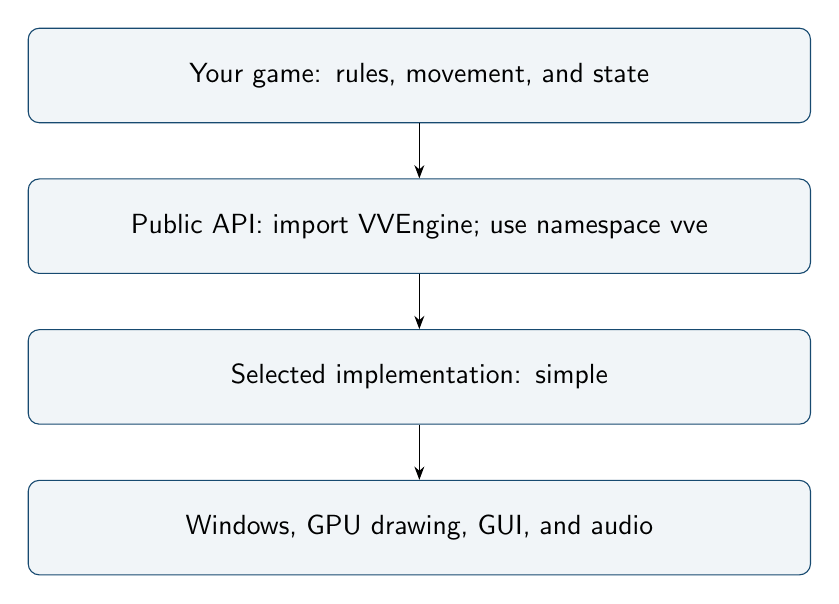
\begin{tikzpicture}[node distance=7mm,every node/.style={draw=vveblue,rounded corners,
    fill=vvelight,text width=0.8\linewidth,align=center,minimum height=12mm,font=\sffamily}]
    \node (game) {Your game: rules, movement, and state};
    \node (facade) [below=of game] {Public API: import VVEngine; use namespace vve};
    \node (engine) [below=of facade] {Selected implementation: simple};
    \node (gpu) [below=of engine] {Windows, GPU drawing, GUI, and audio};
    \draw[-{Stealth}] (game)--(facade);
    \draw[-{Stealth}] (facade)--(engine);
    \draw[-{Stealth}] (engine)--(gpu);
  \end{tikzpicture}\vfill
  {\normalsize Updated 16 October 2026\par}
  {\small Source baseline: 8f875a30; API checked against the local checkout.\par}
  {\small Game code uses the facade. Implementation chapters are for source study.\par}
  \end{titlepage}}

\hypersetup{pdftitle={Vienna Vulkan Engine, explained - expanded beginner edition}}
\setcounter{tocdepth}{1}
\begin{document}
\guidecover{Vienna Vulkan Engine, explained}{An expanded guide from first principles to the source}{Learn what a game engine does, write a small game through the public API, and then follow an object from a file to CPU memory, GPU memory, and a picture. New ideas are explained before they are used. Basic C++ is enough to begin.}

\section*{How to use this book}
This book has two jobs. It teaches you to use VVE, and it explains how VVE's simple implementation carries out your requests. You can learn the public API without first learning Vulkan. Later, the implementation walkthrough connects the public calls to the data and GPU operations behind them.

You should know what a variable, function, \api{if} statement, loop, and simple C++ \api{struct} are. You do not need experience with graphics APIs, shader programming, ECS storage, or C++ modules. The foundations explain the additional vocabulary used in the rest of the guide. When a code example uses modern C++ syntax, nearby text explains the parts that matter.

\textbf{A first project:} read the foundations, build the quickstart's supplied example, and work through the moving-cube program below. Use Part I to find the services you need. Part III explains how to organize an actual game.

\textbf{Reading the engine source:} begin with the CPU/GPU and ownership foundations, then read Part II in order. Keep the source map near the end of the book open beside your editor. A file name is a more lasting starting point than a historical line number.

\textbf{Adding a specific feature:} use the linked contents. Part IV adds detailed current-API recipes for shapes, transparency, skyboxes, sprites, picking, HUD images, audio, scene hierarchies, and diagnosing a missing picture.

\begin{remember}A model file, an imported asset scene, a visible scene instance, and a GPU allocation are different things. Much of engine programming becomes easier once you can say which of these you are changing.\end{remember}

\subsection*{Code labels and scope}
Listings called \emph{complete programs} include their imports and \api{main}. Listings called \emph{excerpts} belong inside the named function or assume the stated variables. File paths in excerpts must name files on your machine. The small built-in-scene and moving-cube programs require no external artwork.

This V3 edition describes the public \api{VVEngine} module and the \api{simple} implementation in the local checkout on 17 October 2026, including the rendering-error, scene-cleanup, builder, and asset-unloading changes. V3 is the repository branch; \api{simple} is the selected implementation. The local source remains the final authority when you change checkout.
\clearpage
\tableofcontents

\clearpage
\part*{Foundations: start here}
\addcontentsline{toc}{part}{Foundations: start here}

\lesson{What the engine does and what your game does}
A game repeatedly answers three broad questions: what did the player do, what changes in the world, and what picture should be shown? Sound and interface updates happen alongside these steps. The repeated cycle is the main loop.

VVE supplies common services: windows, input, asset loading, drawing, GUI integration, and audio. Your game supplies rules. For example, VVE can show a crate and move it to a requested position. Your code decides whether the crate falls, whether the player collected it, and how many points it is worth.

These responsibilities explain why an engine API contains verbs such as \api{addCuboid}, \api{setObjectTransform}, and \api{play}. They describe a request. Your program is not asked to specify Vulkan memory allocations each time it moves a crate. The implementation translates the request into the required internal work.

The \emph{facade} is this public request interface. A facade is an ordinary programming pattern: a small front door to a more complicated system. In VVE the public names live in namespace \api{vve}; the current implementation lives in \api{vve::simple}. Your game uses the front door, even when you study the implementation behind it.

\begin{tabularx}{\linewidth}{@{}p{0.31\linewidth}X@{}}
\toprule Your game decides & VVE carries out \\\midrule
Where the player wants to move & Input polling and the requested visible transform change \\
When an enemy appears & Creating a visible object from geometry and materials \\
When a sound should play & Loading sound data and mixing a playing voice \\
What the score means & Building GUI draw data through the registered callback \\
\bottomrule
\end{tabularx}

You do not need to use every service. A small scene demonstration can use the renderer directly through the facade. A larger game can store entities and components in the ECS and use several user systems. Start with the least code that makes the intended behavior clear.

\begin{tryit}Describe a collectible in two sentences: one about its game rule, another about its appearance. The score belongs to game state; the visible crate handle belongs to the rendering connection.\end{tryit}
\source{src/Engine.ixx; src/World.ixx; src/RenderSystem.ixx}

\lesson{A frame, an update, and elapsed time}
A frame is one iteration of the engine loop. In the public engine, input is polled first. Your registered systems then update in their declared order. Rendering follows. \api{step()} performs one iteration; \api{run()} initializes the engine and repeats steps until stopping or an error.

Think of a frame as a fresh opportunity to describe the world. Input tells you which keys are currently held. Your update changes a position or score. Rendering uses the resulting state to make a picture. This order lets a key press affect the picture produced in that same engine step.

Frames do not all take the same amount of time. A busy frame may take longer than an empty one. If you move by a fixed distance on every frame, the movement speed depends on how quickly the machine produces frames. Use elapsed seconds instead:
\[
\mbox{distance moved}=\mbox{speed in units per second}\times\mbox{elapsed seconds}.
\]
At 3 units per second and a 0.02-second update, the distance is 0.06 units. Over one second, many short updates should add up to approximately 3 units. You choose what a world unit means; using one unit as a metre is a convenient convention, not an engine conversion.

VVE passes a \api{FrameContext} to hooks that ask for it. Read \api{frame.delta_time.seconds} for the elapsed time and \api{frame.frame_index.value} for the zero-based step index. The first delta is the default \api{DeltaTime{}} value, currently 1/60 second; it is not zero. Later deltas come from the steady clock between polls.

The engine's step count and the number of presented pictures are separate. A minimized window can skip presentation while the game keeps updating. A frame cap limits steps. It should not be described as an exact guarantee that a particular number of pictures reached the display.

\begin{tryit}Compare moving by 0.1 units every update with moving by \api{3.0 * dt}. Which stays close to 3 units per second when the frame rate changes?\end{tryit}
\source{src/Engine.ixx; src/Types.ixx; src/versions/simple/Engine.ixx}

\lesson{CPU, GPU, and the two kinds of memory}
The CPU runs your C++ game code. It reads input, updates rules, and prepares work. The GPU runs graphics work in parallel and produces images. They can be busy at the same time, so finishing a C++ function does not always mean that submitted GPU work has finished.

Ordinary C++ containers hold CPU-side data. A model import can produce positions in a vector, triangle indices in another vector, and image bytes in a pixel buffer. These are useful for loading, editing, and inspection. They are not automatically the Vulkan resources used for drawing.

The renderer creates GPU buffers for vertex and index data, images for textures and render targets, and bindings that tell shaders where to read. \emph{Uploading} means arranging for data prepared by the CPU to be copied into resources the GPU will use. Some memory is visible to both processors, but it still needs an explicit usage and synchronization policy.

\begin{center}
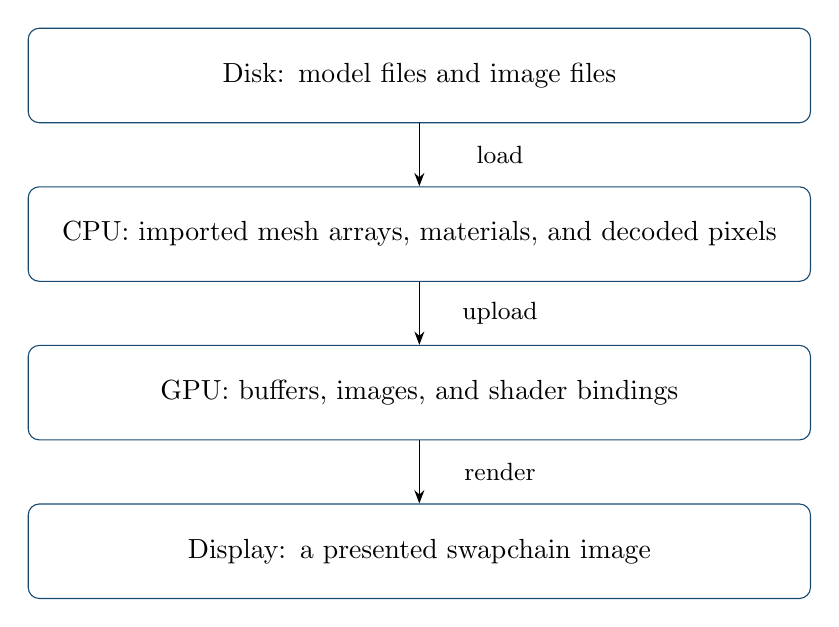
\begin{tikzpicture}[node distance=8mm,every node/.style={draw=vveblue,rounded corners,align=center,text width=0.8\linewidth,minimum height=12mm}]
\node (file) {Disk: model files and image files};
\node (cpu) [below=of file] {CPU: imported mesh arrays, materials, and decoded pixels};
\node (gpu) [below=of cpu] {GPU: buffers, images, and shader bindings};
\node (screen) [below=of gpu] {Display: a presented swapchain image};
\draw[-{Stealth}] (file)--node[right,draw=none,text width=18mm,font=\small]{load} (cpu);
\draw[-{Stealth}] (cpu)--node[right,draw=none,text width=18mm,font=\small]{upload} (gpu);
\draw[-{Stealth}] (gpu)--node[right,draw=none,text width=18mm,font=\small]{render} (screen);
\end{tikzpicture}
\end{center}

VVE keeps those stages separate so it can share geometry, delay work until rendering needs it, and remove resources safely. The later source walkthrough follows each stage. As a game programmer, first learn which public call loads data and which creates a visible placement.

\begin{remember}A handle returned by an asset load does not prove that the GPU already contains the model, or that the model has been drawn. It identifies a successful stage in the process.\end{remember}
\source{src/versions/simple/Assets.ixx; src/versions/simple/Render/RenderResources.ixx; src/versions/simple/Render/RendererResources.cpp}

\lesson{Vertices, triangles, meshes, and materials}
A vertex is a point with attributes. Its position says where it is. A normal describes a surface direction for lighting. Texture coordinates say which location in an image should be sampled. Not every mesh supplies every attribute; the renderer has defined fallbacks for some missing information.

Three vertices define a triangle. A mesh is a reusable collection of vertices and triangles. Instead of storing a full vertex three times for each triangle, an index array can name vertices already stored in the vertex array. For example, indices \api{0,1,2} draw a triangle using the first three vertices. Two triangles can share corner vertices when their attributes match.

A material describes surface appearance. It can contain a base colour, texture references, and factors used by lighting. A texture is an image sampled by the shader. Geometry and appearance are different resources: the same cube mesh can appear in green, blue, or with a crate image.

A visible object combines reusable resources with placement and state. Two crates can share mesh and material data while having different transforms. Moving one should change its placement, not force a second copy of every vertex.

\begin{tabularx}{\linewidth}{@{}p{0.25\linewidth}X@{}}
\toprule Name & A useful mental picture \\\midrule
Vertex & One corner plus the data attached to it \\
Index & A number naming a stored vertex \\
Mesh & Reusable shape made of triangles \\
Material & Instructions and data for surface appearance \\
Texture & Image used by a material or interface \\
Render object & One visible use of geometry and appearance at a placement \\
\bottomrule
\end{tabularx}

The public API offers plane, cuboid, sphere, sprite, and mesh creation so you can learn without building an asset pipeline first. Later, \api{AssetSystem::loadScene} imports a model file containing meshes, materials, and a hierarchy of parts.

\begin{tryit}If a level contains 100 identical crates, how many placements does it need? It needs 100 placements. Sharing may allow the geometry and appearance resources to be stored only once.\end{tryit}
\source{src/Types.ixx; src/RenderSystem.ixx; src/versions/simple/Types.ixx}

\lesson{Coordinates and local versus world space}
A three-dimensional position has X, Y, and Z coordinates. In this guide, Y points up. X moves across the ground and Z measures the other ground direction. The default camera looks along negative Z. The numbers are meaningful relative to a coordinate system.

\emph{Local space} describes an object before placement. A cube from -0.5 to +0.5 on all axes is one unit wide, centred on its own origin. \emph{World space} describes where the placed object is in the scene. Translating the cube to Y=0.5 makes its bottom touch a ground plane at Y=0.

A \api{Transform} contains translation, rotation, and scale. Translation moves the object. Rotation turns it around its local origin. Scale changes its size. The default translation is zero, the default rotation changes no direction, and the default scale is one on every axis.
\begin{lstlisting}
vve::Transform pose{};
pose.translation.value = vve::Vec3{2.0F, 0.5F, 0.0F};
pose.scale.value = vve::Vec3{1.0F, 2.0F, 1.0F};
\end{lstlisting}
Here the local cube is stretched to two units high, then placed with its centre at Y=0.5. Its bottom would be below the ground. To rest this stretched cube on the ground, use centre Y=1. This small calculation is useful when an imported model appears partly buried.

Hierarchy introduces another local relationship. A wheel's local transform is relative to its parent car node. Moving the car changes the world position of the wheel without changing the wheel's local offset. You do not need matrix algebra to use this relationship; the scene tree combines the transforms for you.

VVE uses strong wrappers such as \api{Position} and \api{Scale}. The nested \api{.value} accesses the contained vector. This extra name helps distinguish a position from a direction even though both contain three numbers.

\begin{tryit}A one-unit cube should rest on a platform at Y=4. What is its centre height? Answer: 4.5, before any additional scaling or parent transform.\end{tryit}
\source{src/Types.ixx; src/Math.ixx; src/versions/simple/Render/RenderSystemScene.cpp}

\lesson{A camera is a view, not a visible object}
A camera describes where the view begins and which way it points. It also defines the vertical field of view and near/far clipping distances. These values turn a three-dimensional world into a two-dimensional picture. Changing the camera does not move the scene's objects.

\api{Camera::lookAt} is a useful starting point because you can name a position and a target instead of computing the forward direction yourself:
\begin{lstlisting}
auto camera = vve::Camera::lookAt(
    vve::Position{.value = vve::Vec3{0.0F, 3.0F, 7.0F}},
    vve::Position{.value = vve::Vec3{0.0F, 0.5F, 0.0F}});
render.setCamera(camera); // Excerpt: render is a RenderSystem reference.
\end{lstlisting}
The camera sits above and in front of a small object near the origin. Its forward vector is the target minus the camera position. Use different positions for a model whose centre or scale differs. A camera position and target at the same point do not define a useful viewing direction.

The field of view controls how wide the view feels. The window's aspect ratio is width divided by height; VVE uses each rendered window's own drawable size for it. The public camera stores a direction rather than an ECS camera binding. Its compatibility \api{up} argument does not store arbitrary camera roll; the renderer chooses a stable up basis.

Clipping removes geometry too near or too far from the camera. The default near distance is 0.1 and the far distance is 100. If a castle is thousands of units across, this range is too small. Change \api{camera.clip} and choose a suitable viewing distance. Avoid choosing a tiny near distance merely to compensate for a poor model scale.

\begin{remember}When the window is empty, first check the object's position, the camera position and direction, and the clipping range. Successfully loading a file cannot guarantee good framing.\end{remember}
\source{src/Types.ixx; src/RenderSystem.ixx; examples/sponza/SponzaCamera.hpp}

\lesson{References, owners, and handles}
An owner is responsible for keeping a resource alive and eventually releasing it. A reference provides access to something that already exists. A handle identifies something managed elsewhere. These are three different relationships.

The public \api{Engine} owns its concrete engine implementation. That implementation owns its window, asset, render, GUI, audio, and ECS services. Public subsystem wrappers hold references to those implementation objects. Getting a wrapper does not create another renderer or transfer ownership.
\begin{lstlisting}
auto world = engine.world();
auto &render = world.get<vve::RenderSystem>();
\end{lstlisting}
The \api{&} means \api{render} refers to the existing wrapper stored by the engine. \api{World} is a bundle of references, so it is cheap to obtain. It must not outlive the engine whose services it exposes. Keeping a world after returning a local engine from a function would leave dangling references.

A \api{RenderObjectHandle} is an ID returned when an object is created. Copying the handle copies only the ID. It neither duplicates the object nor keeps a removed object alive. Passing a removed handle to an operation fails according to that operation's error contract. The handle's \api{valid()} method checks its nonzero representation; it cannot by itself prove that the resource still exists.

Handle types prevent category mistakes. A \api{SceneHandle} is not a \api{RenderSceneInstanceHandle}, and an asset \api{NodeHandle} is not a world-tree \api{SceneNodeHandle}. The compiler helps catch mixing these up before the game runs.

\api{Vector<T>} is VVE's name for \api{std::vector<T>}. Growing a vector can move its elements. Borrowed pointers and references into it may then become invalid. Public asset queries generally return owning values; implementation-only borrowed views have shorter lifetimes.

\begin{tryit}If you copy a crate's handle and then call \api{removeObject}, do either of the two copies keep the crate alive? No. Both copies identify the same removed resource.\end{tryit}
\source{src/Engine.ixx; src/World.ixx; src/Handle.ixx; src/Vector.ixx}

\lesson{Read the modern C++ syntax used in examples}
\api{auto} asks the compiler to work out a variable's type from its initial value. It does not make the value untyped. In \api{auto scene = assets.loadScene(path)}, the result still has a precise \api{std::expected} type. \api{auto &render} adds a reference to the existing object.

Braces create and initialize values. \api{vve::PixelExtent{800, 600}} fills width and height in declaration order. A designated initializer names the field: \api{vve::Position{.value = vve::Vec3{0, 1, 0}}}. The name helps explain which nested value is being set. C++ designated initializers follow declaration order when several fields are named.

Angle brackets supply template arguments. \api{Engine<Game>} means an engine owning a user system of type \api{Game}. \api{world.get<vve::RenderSystem>()} asks for the stored service of that type. These arguments are types chosen at compile time, not strings looked up each frame.

A function parameter \api{auto &world} makes that function generic. Because C++ does not yet know the exact type of \api{world}, write \api{world.template get<vve::RenderSystem>()}. The extra keyword tells the parser that \api{get<...>} is a template call. Ordinary non-generic code uses \api{world.get<...>()}.

A lambda is a small function value. The expression \api{[this] { ... }} makes a callback that can use the current object's members. A GUI callback runs later, so captured state must still exist when it runs. Capturing a reference to a temporary local variable is not a safe way to preserve that variable.

The statement \api{if (const auto result = operation(); !result)} first calls an operation, then checks failure. The variable lives through the \api{if} statement. The \api{-> std::expected<void, vve::Error>} spelling is a trailing return type; it says what the function returns.

\begin{remember}Read a listing for its data flow first: obtain a service, make a request, check its result, retain any useful handle. You can study the template machinery later.\end{remember}
\source{src/Engine.ixx; src/World.ixx; src/Types.ixx}

\lesson{Handle an operation that may fail}
Files can be missing, a handle can be unknown, and a platform operation can fail. VVE represents many such outcomes with \api{std::expected<Value, vve::Error>}. It contains either the requested value or an error enum. An enum is a named category, such as \api{io_error}, rather than a full descriptive sentence.
\begin{lstlisting}
auto created = render.addSphere(1.0F, vve::LinearColor{});
if (!created) {
    std::cerr << "Could not add sphere: "
              << vve::errorName(created.error()) << '\n';
    return 1; // This excerpt belongs in an int-returning function.
}
const vve::RenderObjectHandle sphere = *created;
\end{lstlisting}
The \api{if} checks before the dereference. On success, \api{*created} is the sphere's handle. On failure, \api{created.error()} supplies the error category. Do not ask for the value before checking success, or ask for the error on a successful result.

For an operation with no result value, use \api{std::expected<void, vve::Error>}. Success is an empty successful result, often written \api{return {};}. A user-system hook can propagate an error with \api{return std::unexpected(result.error());}. That stops later hooks and rendering for the current step.

\api{std::optional<T>} is different. It has a value or no value, without an error category. \api{findWindow} can return no window; \api{raycast} can return no hit. An ordinary miss is not necessarily a failure.

During development, add context when reporting an error. \emph{Could not load level assets/room.gltf: asset\_import\_failed} tells you more than a lone number. Audio also supplies \api{lastError()} for a more detailed diagnostic.

A successful step can include a temporarily skipped drawing attempt, for example while a window is minimized or acquisition times out. Fatal rendering failures follow a different path: they propagate as errors through \api{RenderSystem} to \api{Engine::step()} and \api{run()}. Check those results; use rendered-frame counts and captures when you need evidence that a picture was presented.
\source{src/Error.ixx; src/Engine.ixx; src/Audio.ixx; src/versions/simple/Render/RendererDraw.cpp}

\lesson{Build tools and files: a practical mental model}
The repository has source files, assets, build directories, and final executables. Keeping their roles separate helps you diagnose the first failure rather than guessing at game code.

CMake reads \api{CMakeLists.txt} files and generates a build description. Ninja executes that description. The compiler translates C++ units, including modules, and the linker combines compiled code and libraries into a usable program. The normal build scripts also arrange dependencies and run CTest.

vcpkg supplies libraries such as SDL3, Assimp, and ImGui. The Vulkan SDK supplies Vulkan tooling and Slang, the compiler used for the renderer's shaders. The post-processing library vvppl is fetched from a pinned archive, unless an offline source override is configured. Matching dependencies and compiler settings matter especially for module builds.

An \api{.ixx} file is a C++ module interface unit in this project. A game imports \api{VVEngine}; it does not include the \api{.ixx} file as a textual header. CMake tracks which module interfaces each compilation needs. A \api{.cpp} file can be an ordinary program or a module implementation unit.

The selected implementation is a CMake choice: \api{VVE_ENGINE_IMPLEMENTATION_NAMESPACE=simple}. Template arguments to \api{Engine<...>} choose user-system types, not the concrete renderer. There is currently only one implementation available.

\begin{tabularx}{\linewidth}{@{}p{0.28\linewidth}X@{}}
\toprule Folder & Contents \\\midrule
\path{src/} & Facade modules and shared vocabulary \\
\path{src/versions/simple/} & Simple engine implementation and shaders \\
\path{examples/} & Programs that use the public facade \\
\path{tests/} & Registered C++ tests and shared test support \\
\path{build/<variant>/} & Generated build files; exact directory names vary by script or preset \\
\path{bin/debug/exe/} & Debug executables; release uses \path{bin/release/exe/} \\
\bottomrule
\end{tabularx}

\begin{tryit}Find the executable for one successful example and the CMake file that creates its target. Explain why importing a module and linking a library are both needed.\end{tryit}
\source{README.md; CMakeLists.txt; src/CMakeLists.txt}

\lesson{A complete moving-cube program: creation}
Create an example target as described in the quickstart. The following listing and the next page form one complete \path{main.cpp}. The cube needs no external assets. Start with an unlit colour so that lighting cannot hide your first object.
% doc-example: moving_cube_begin
\begin{lstlisting}
import std;
import VVEngine;

struct MovingCube {
    vve::RenderObjectHandle cube{}; // ID of the visible cube.
    vve::Transform pose{};         // Game-owned desired placement.

    auto init(auto &world) -> std::expected<void, vve::Error> {
        auto &render = world.template get<vve::RenderSystem>();
        render.setBackgroundColor(vve::LinearColor{
            .value = vve::Vec3{0.08F, 0.12F, 0.18F}});
        render.setCamera(vve::Camera::lookAt(
            vve::Position{.value = vve::Vec3{0, 2, 6}},
            vve::Position{.value = vve::Vec3{0, 0, 0}}));
        auto created = render.addCuboid(
            vve::Vec3{-0.5F, -0.5F, -0.5F},
            vve::Vec3{ 0.5F,  0.5F,  0.5F},
            vve::LinearColor{
                .value = vve::Vec3{0.2F, 0.8F, 0.4F}}, pose);
        if (!created) { return std::unexpected(created.error()); }
        cube = *created;
        return render.setObjectUnlit(cube, true);
    }
\end{lstlisting}
\api{cube} and \api{pose} are members because the update needs them after \api{init} returns. A local variable inside \api{init} would not preserve that state for the next frame. The engine owns one \api{MovingCube} object for the application's lifetime.

The minimum and maximum corners describe a one-unit local cube. \api{pose} places it at the origin. The camera looks from positive Z toward that origin. The background is dark and the cube is green, making the result easy to recognize.

The two operations that can fail are checked: cube creation and setting its unlit flag. Returning the latter result forwards either success or its error without an additional branch.
\source{src/RenderSystem.ixx; src/Types.ixx}

\lesson{A complete moving-cube program: update and main}
Continue the same \path{main.cpp} directly after the previous listing:
% doc-example: moving_cube_end
\begin{lstlisting}
    auto update(auto &world, const vve::FrameContext &frame)
        -> std::expected<void, vve::Error> {
        auto input = world.template get<vve::WindowSystem>().input();
        const float dt = static_cast<float>(
            std::clamp(frame.delta_time.seconds, 0.0, 0.1));
        float direction = 0.0F;
        if (input.isKeyDown(vve::Key::a)) { direction -= 1.0F; }
        if (input.isKeyDown(vve::Key::d)) { direction += 1.0F; }
        pose.translation.value.x += direction * 2.0F * dt;
        return world.template get<vve::RenderSystem>()
            .setObjectTransform(cube, pose);
    }
};

int main() {
    auto engine = vve::EngineBuilder<MovingCube>{}
        .applicationName("Moving cube")
        .addWindow(vve::WindowSetup{}.id("main")
            .title("A / D move the cube")
            .extent(vve::PixelExtent{800, 600}))
        .build();
    if (const auto result = engine.run(); !result) {
        std::cerr << vve::errorName(result.error()) << '\n';
        return 1;
    }
    return 0;
}
\end{lstlisting}
\textbf{Expected result:} a green cube on a dark background. Focus the window. Holding A moves the cube left; holding D moves it right. Holding both cancels the requested movement. Close the window to stop the program.

The game updates its own \api{pose}, then submits that placement to the renderer. This is the simplest form of gameplay-to-render synchronization. Nothing automatically ties a C++ position member to a visible object.

The elapsed-time clamp prevents a long pause, such as stopping at a debugger breakpoint, from producing a large jump in this teaching example. It deliberately sacrifices catching up that lost time. A game needing stable simulation can use an accumulator and fixed steps instead; Part III explains that approach.

\begin{tryit}Change speed 2 to 4. Change the green colour. Add W/S movement along Z. Make one change at a time and check its visible result.\end{tryit}
\source{src/Engine.ixx; src/Window.ixx; src/Types.ixx}

\lesson{Predict one complete trip through the loop}
Suppose the cube starts at X=0. You hold D, and the next update receives 0.02 seconds. Before the update runs, the engine polls platform events. \api{isKeyDown(Key::d)} now observes the held key. The update computes direction +1 and moves by \api{1 * 2 * 0.02}, or 0.04 units.

\api{setObjectTransform} stores the requested placement in the CPU render scene. It does not recreate the cube's local vertex positions. Later in the same engine step, rendering builds object draw data using that placement. The shared cube geometry can remain unchanged on the GPU.

The CPU records commands, submits them to a GPU queue, and arranges presentation. These operations are ordered using synchronization objects. There may be older GPU work still running while your next update is being prepared. This is why the renderer keeps frame resources and tracks which submitted work has completed.

On the first render, more work happens: the engine creates the Vulkan device and per-window resources, uploads geometry, and sets up pipelines. Later frames usually reuse those resources. Startup can therefore be more expensive than a steady-state frame even for a tiny game.

If you minimize the window, the engine can skip drawing while keeping the scene and target resources. Restoring it should not require reconstructing every game object. Your update code should not interpret a skipped presentation as a command to reset the game.

\begin{enumerate}
\item Poll: turn platform events into usable input state.
\item Update: change game-owned state.
\item Synchronize: send the desired visible state to render objects.
\item Render: prepare resources and commands for drawable windows.
\item Present: give a completed image to the window system.
\end{enumerate}
\begin{remember}Keep this sequence in mind while reading the detailed source chapters. Each internal class exists to carry out one or more of these steps safely.\end{remember}
\source{src/Engine.ixx; src/versions/simple/Engine.ixx; src/versions/simple/Render/RendererDraw.cpp}

% BEGIN REVIEWED FACADE, IMPLEMENTATION, AND GAME WALKTHROUGH
\clearpage\part{The public facade}
\lesson{What the facade gives you}\label{core-4}
A single public interface connects your game to the selected engine.

A facade is the set of classes and functions your game calls. In Vienna Vulkan Engine, start with import VVEngine; and use names in namespace vve. The module name is VVEngine; the central C++ class is vve::Engine. They are different kinds of names.

The cover diagram shows the request path from the game through the facade and selected implementation to the platform.

\subsection*{Say what you want to happen}
Call addTexturedPlane() to make ground, setObjectTransform() to move an object, or setCamera() to choose a view. The facade forwards each request to the implementation. The implementation decides how to store geometry, upload pixels, allocate Vulkan resources and draw the result.

\subsection*{The interface also supplies a shared vocabulary}
Transform, Position, Camera, typed handles and Error describe requests and results. They carry useful meaning without exposing the internal Catalog, RenderScene or Vulkan device. The ECS is shared public storage for your own component types.

{\small
\begin{longtable}{@{}p{0.42\linewidth}p{0.54\linewidth}@{}}
Layer & Names you will encounter \\
Game-facing interface & vve::Engine, World, AssetSystem, RenderSystem, WindowSystem, GuiSystem, ECS \\
Selected implementation & vve::simple::Engine and its window, asset, GUI and rendering classes \\
Implementation details & Catalog, RenderMesh, ForwardRenderer, WindowTarget and Vulkan resource owners \\
\end{longtable}
}

\subsection*{How to read this book}
Part I explains the public classes and their contracts. Part II follows the simple engine behind those contracts. Part III shows how to build a game with them. Implementation-specific behavior is identified where it matters.
\source{src/Engine.ixx; src/implementations/simple.ixx}

\lesson{Facade classes: who provides API calls?}\label{core-5}
The public layer contains service APIs, construction helpers and data types.

{\small
\begin{longtable}{@{}p{0.42\linewidth}p{0.54\linewidth}@{}}
Class / template & API role and state \\
Engine<TSystems...> & API: lifecycle, world lookup and frame context. Owns one implementation and the user systems. \\
EngineBuilder<TSystems...> & Construction API: collects startup options and builds an Engine. \\
World<TObjects...> & Access API: get<T>() returns a reference to an existing service or user system. \\
AssetSystem & Service API: imports and queries source scene, node, mesh, material, light and camera data. \\
RenderSystem & Service API: creates visible objects; controls placement, cameras, lighting, effects and capture. \\
WindowSystem & Service API: lists/finds windows and hands out input access. \\
Window & Read-only API: handle, identity, extent, renderer and current platform state. \\
InputState & Input API: key and per-window mouse queries; also exposes input-state mutation methods. \\
GuiSystem & Service API: registers GUI and font callbacks, loads HUD images, and returns image IDs. \\
AudioSystem & Service API: opens audio, loads sounds, starts voices, and controls playback and gain. \\
BasicECS<TTraits> / ECS & Storage API: creates entities and adds, reads, writes, removes or selects components. \\
DefaultCameraController & Utility API: turns keyboard input and elapsed time into a Camera. \\
WindowSetup / WindowSetups & Configuration API: fluent window settings and a startup window collection. \\
UserSystems<T...> & Data: tuple of user-system values supplied to Engine. \\
MakeUserSystems / makeUserSystems & Utility API: builds a correctly typed UserSystems bundle from values. \\
DefaultECSTraits & Configuration type: selects ECS storage behavior; slot maps are not implemented here. \\
TypedHandle<Tag> / HandleHash & Value/utility API: typed identity queries and hashing; no resource ownership. \\
Camera and descriptor structs & Data, with a few convenience helpers such as Camera::lookAt(). \\
\end{longtable}
}

An API method can read state as well as change it. A struct with fields is also part of the public contract, but filling in that struct does not create a window, object or GPU resource until you pass it to the appropriate service.
\source{src/Engine.ixx; src/World.ixx; src/Audio.ixx}

\lesson{Engine: the owner and coordinator}\label{core-6}
The facade Engine keeps one implementation and your registered systems alive.

Engine<TSystems...> combines engine services with the concrete types of your game systems. Engine<> has no registered game systems. Engine<Movement, Score> owns one Movement and one Score in a tuple. The template parameters describe the game systems; they do not choose the rendering implementation.

{\small
\begin{longtable}{@{}p{0.42\linewidth}p{0.54\linewidth}@{}}
Public call & Meaning \\
init() & Initialize the implementation, then run optional user init hooks. Return expected<void,Error>. \\
step() & Poll/update backend state, call user updates, render, then return running/stopped or an error. \\
run() & Call init and repeat step until stopped or an error occurs. \\
world() & Create a small reference view of the existing services and user systems. \\
frameContext() & Read the latest polled frame index and delta time. \\
versionMajor() / & Read implementation version information. versionName() \\
\end{longtable}
}

\subsection*{What is stored inside}
A unique\_ptr owns the selected EngineImpl. The facade stores a reference to the ECS and lightweight wrappers for assets, GUI, audio, windows and rendering. It separately owns your user-system tuple and remembers how many init hooks completed successfully.

\subsection*{Keep the engine at a stable address}
Engine cannot be copied or moved. Its wrapper references must continue to refer to the same underlying subsystem objects. The builder returns a newly constructed Engine directly, using C++ guaranteed copy elision; it does not move an already existing engine.

\subsection*{Construction is not full initialization}
Constructing Engine creates the C++ owners and connections. Call init() before step(). In the simple implementation, platform/windows initialize first and the renderer creates GPU resources lazily when rendering starts.
\source{src/Engine.ixx}

\lesson{All public ways to create an engine}\label{core-7}
Choose default construction, typed options or a fluent builder.

\begin{lstlisting}[language={}]
import std;
import VVEngine;

vve::Engine<> defaults;

vve::Engine<> configured{
    vve::ApplicationName{.value = "My game"},
    vve::MaxFrames{.value = vve::FrameCount{.value = 120}}
};

auto built = vve::EngineBuilder<>{}
    .applicationName("My game")
    .addWindow(vve::WindowSetup{}
        .id("main").title("My game")
        .extent({.width = 1280, .height = 720}))
    .build();
\end{lstlisting}

{\small
\begin{longtable}{@{}p{0.42\linewidth}p{0.54\linewidth}@{}}
Choice & What to supply \\
Defaults & Engine<> or Engine<YourSystem...> with default-constructible systems. \\
Direct typed options & ApplicationName, MaxFrames, WindowSetups and a matching UserSystems bundle. \\
\end{longtable}
}

{\small
\begin{longtable}{@{}p{0.42\linewidth}p{0.54\linewidth}@{}}
Builder & applicationName(string), maxFrames(MaxFrames), windows(WindowSetups), addWindow(WindowSetup), userSystems(UserSystems). \\
\end{longtable}
}

{\small
\begin{longtable}{@{}p{0.42\linewidth}p{0.54\linewidth}@{}}
Explicit system values & Engine<Game>\{makeUserSystems(Game\{...\})\}; supply the same system types and order as Engine. \\
\end{longtable}
}

These are alternative construction examples, not a recommendation to create three engines in one application. They all reach the same factory and implementation. An unknown direct option type causes a compile error. Repeated name/frame/window options are processed in order, with the later value replacing the earlier value.

\subsection*{MaxFrames is a step limit}
A value of zero means no configured frame cap. This option does not set frames per second. Use run() for engine-controlled execution, or init() and step() when your application owns the loop.
\source{src/Engine.ixx}

\lesson{Engine creation, one step at a time}\label{core-8}
CMake selects a concrete type; the factory allocates an object of that type.

\subsection*{Implementation}
CMake setting                                          makeEngineImpl()            Facade constructor aliases simple                                                 new owner                  service references EngineImpl

1. Configure the build. VVE\_ENGINE\_IMPLEMENTATION\_NAMESPACE selects src/implementations/<name>.ixx and the corresponding engine source folder. The current repository supplies only simple. Selecting a new name requires an actual compatible implementation and adapter; changing the setting alone cannot create one. 2. Compile the adapter. The simple adapter defines detail::EngineImpl as simple::Engine, and matching aliases for every wrapped subsystem. An alias names the concrete type. It is not an allocated object and it is not a runtime plugin selector. 3. Collect options. The facade extracts ApplicationName, MaxFrames and optional window descriptors. UserSystems are retained for the later system-tuple setup rather than passed into the backend factory. 4. Allocate the implementation. Inline detail::makeEngineImpl() calls make\_unique<EngineImpl>. With explicit windows it also passes WindowsImpl containing their descriptors; otherwise it uses the constructor without that argument. The resulting unique\_ptr is the facade owner. 5. Bind services and systems. The facade obtains impl\_->ecs(), assets(), gui(), windowSystem() and renderSystem(). It constructs wrappers referring to those objects. Then it copies/moves the supplied user-system bundle or default-constructs the systems.

\begin{lstlisting}[language={}]
// The selected adapter establishes the type:
using EngineImpl = simple::Engine;

// The factory creates an object of that type:
return std::make_unique<EngineImpl>(name, max_frames);
\end{lstlisting}

\subsection*{How a call finds the real state}
The alias tells the compiler which methods exist. The stored object supplies the state those methods operate on. A RenderSystem wrapper holds a reference to a real RenderSystemImpl, and forwards calls to that instance. There is no virtual dispatch or runtime engine switch in this design.
\source{src/Engine.ixx}

\lesson{World: references to the stored objects}\label{core-9}
get() finds an existing object by its exact C++ type.

\begin{lstlisting}[language={}]
auto world = engine.world();
auto& render = world.get<vve::RenderSystem>();
auto& assets = world.get<vve::AssetSystem>();
auto& windows = world.get<vve::WindowSystem>();
auto& gui = world.get<vve::GuiSystem>();
auto& ecs = world.get<vve::ECS>();
// With Engine<Game>, also: world.get<Game>()
\end{lstlisting}

World<TObjects...> contains a tuple of reference\_wrapper values. Engine creates the view from references to its ECS, public subsystem wrappers and user-system objects. There is no separate World implementation and no second scene stored inside World.

\subsection*{Type lookup and object access are separate jobs}
get<RenderSystem>() searches the tuple at compile time for that exact target type. It then returns the stored reference. Calling render.setCamera() uses the wrapper object you obtained; the wrapper forwards to its stored implementation reference. The type determines the method, and the object supplies its actual state. A missing type is a compile error. If a type appears more than once, get<T>() finds the first one, so use distinct system types when you need to access them individually. In templated hooks, write world.template get<T>() because the World type depends on a template parameter.

\subsection*{Lifetime and constness}
A World can be move-constructed, but cannot be copied or assigned. It is cheap to obtain another one from engine.world(). Its references remain usable only while the engine and the referred objects live. Making the view const does not freeze the objects referred to by its reference wrappers.

\subsection*{Copies of subsystem wrappers are still views}
AssetSystem, RenderSystem, WindowSystem, GuiSystem, InputState and Window allow copy/move construction but delete assignment. Copying one does not duplicate an asset catalog or GPU scene. Window is read-only; the other wrappers retain access to the same implementation state.
\source{src/World.ixx}

\lesson{UserSystems and automatic hooks}\label{core-10}
The engine calls ordinary methods on the system values it owns.

\begin{lstlisting}[language={}]
struct Game {
    int score = 0;
    template<class W> void init(W& world) {
        // Prepare game state through public services.
    }
    template<class W>
    void update(W& world, const vve::FrameContext& frame) {
        // Read input, advance game state, publish transforms.
    }
};
vve::Engine<Game> engine{vve::makeUserSystems(Game{})};
\end{lstlisting}

UserSystems<T...> is a tuple of system values. The callable object makeUserSystems (type MakeUserSystems) deduces concrete types and forwards the supplied values into that tuple. No base class, virtual method or registration name is required.

{\small
\begin{longtable}{@{}p{0.42\linewidth}p{0.54\linewidth}@{}}
Available hook & When / priority \\
init(world) & Optional, called after backend init, in tuple order. \\
update(world, frame, window\_frame) & Highest update priority; receives current copied WindowFrameData. \\
update(world, frame) & Next priority; receives current FrameContext. \\
update(world) & Next priority; needs no frame arguments. \\
No matching hook & No call for that stage. \\
\end{longtable}
}

Only the highest matching update overload is called for a system. Hooks run in tuple order on the engine-owned values, not on an original object that was copied into a bundle. Window snapshots are prepared only if at least one system accepts the three-argument update. A hook may return void or std::expected<void,Error>. Only that exact expected type propagates failure; other return values are discarded. A failing init is retried on the next init() while earlier successful hooks stay complete. A failing update stops later systems and rendering for that step.

\clearpage
\subsection*{Copies, moves and builders}
Direct construction with a temporary bundle can move system values, including move-only state. The builder supports two paths: \api{builder.build()} copies a named builder and requires copyable systems; \api{std::move(builder).build()} consumes it and moves its systems. A temporary fluent chain also uses the consuming path. A system without a default constructor needs an explicitly supplied \api{UserSystems} bundle, passed to the engine or builder constructor.

\begin{lstlisting}
// Excerpt: inside main, after importing std and VVEngine.
struct GameState {
    std::unique_ptr<int> score;
    explicit GameState(std::unique_ptr<int> value)
        : score{std::move(value)} {}
};
auto builder = vve::EngineBuilder<GameState>{
    vve::makeUserSystems(GameState{std::make_unique<int>(0)})};
auto engine = std::move(builder).build();
\end{lstlisting}
Here the engine owns the original score allocation. After consuming the builder, do not expect it to retain its previous systems or startup values. The Engine itself is still constructed directly in its destination; no Engine move constructor is needed.
\source{src/Engine.ixx}

\lesson{WindowSetup and WindowSetups}\label{core-11}
These helpers describe windows before initialization creates them.

\begin{lstlisting}[language={}]
vve::WindowSetups windows{
    vve::WindowSetup{}.id("main").title("Player")
        .extent({.width = 1280, .height = 720})
        .resizable(true).visible(true),
    vve::WindowSetup{}.id("map").title("Map")
        .extent({.width = 640, .height = 480})
        .renderer(vve::RendererId{.value = "forward"})
};
vve::Engine<> engine{std::move(windows)};
\end{lstlisting}

{\small
\begin{longtable}{@{}p{0.42\linewidth}p{0.54\linewidth}@{}}
Setting & Meaning / default \\
id(string) & Application-local lookup name. Default main; must be nonempty and unique. \\
title(string) & Visible title. Default VVE simple; the simple engine substitutes the application name for the default title. \\
extent(PixelExtent) & Initial window-coordinate size, default 960 x 540; nonzero dimensions required. \\
position(x,y) & Optional screen position; otherwise leave platform placement unspecified. \\
renderer(RendererId) & Empty or forward draws; none opts out. Unknown identifiers fail init. \\
resizable(bool) / visible(bool) & Both default true. Hidden windows can still render for captures/tests. \\
\end{longtable}
}

{\small
\begin{longtable}{@{}p{0.42\linewidth}p{0.54\linewidth}@{}}
WindowSetups::add(WindowSetup) & Append a startup descriptor. An empty collection gets a default main window. \\
\end{longtable}
}

WindowSetup owns one WindowDesc. WindowSetups owns the collection. Fluent methods return a reference to the same helper so you can chain settings; they do not immediately contact SDL or create a native window.

\subsection*{Startup size versus drawable size}
Startup extent uses window coordinates. Window::extent() later reports drawable pixels, which can differ on a scaled display. The renderer uses drawable pixels for its swapchain and aspect ratio. These startup helpers do not expose runtime window creation or resizing commands.
\source{src/Window.ixx}

\lesson{WindowSystem and Window}\label{core-12}
The manager returns small read-only views of the windows it owns.

\begin{lstlisting}[language={}]
auto world = engine.world();
auto& windows = world.get<vve::WindowSystem>();
auto main = windows.findWindow("main");
if (main) {
    auto handle = main->handle();
    auto drawable_size = main->extent();
    // Save the handle for camera, mouse and capture APIs.
}
\end{lstlisting}

{\small
\begin{longtable}{@{}p{0.42\linewidth}p{0.54\linewidth}@{}}
WindowSystem call & Result \\
name() & Window backend name as a string\_view. \\
windowCount() & Number of windows in the manager. \\
windows() & Vector of Window wrappers; wrappers still refer to owned windows. \\
findWindow(id) / findWindow(handle) & optional<Window>; empty when lookup fails. \\
input() & InputState wrapper over the same live input object. \\
Window call & What it reads \\
handle(), id(), title() & Typed runtime identity, stable application ID and platform title. \\
extent(), rendererId() & Drawable pixel dimensions and renderer selection. \\
focused(), minimized(), shouldClose() & State from platform events. \\
\end{longtable}
}

Window stores a const implementation reference. It has no public setTitle, resize or destroy call. WindowSystem owns window management; a Window value gives you access to state, not ownership of the native resource. string\_view results also borrow the underlying strings.

\subsection*{Current simple-engine behavior}
A close request on any managed window stops the engine. A minimized or zero-size target can skip drawing; a hidden target can still draw. Each rendering window has its own swapchain and aspect ratio. Cameras are controlled through RenderSystem, not Window or ECS camera bindings.

\subsection*{Live view versus snapshot}
Reading Window after event polling sees the refreshed state. WindowFrameData, supplied to an optional three-argument system hook, owns copies of WindowInfo for that frame. Keeping a Window wrapper is not the same as keeping a historical snapshot.
\source{src/Window.ixx}

\lesson{InputState and DefaultCameraController}\label{core-13}
Use frame edges for actions and held state for continuous movement.

{\small
\begin{longtable}{@{}p{0.42\linewidth}p{0.54\linewidth}@{}}
InputState query & Meaning \\
isKeyDown(Key or keycode) & Held now; useful for walking or continuous movement. \\
wasKeyPressed(Key or keycode) & Press edge in the current poll; useful for one action. \\
wasKeyReleased(Key or keycode) & Release edge in the current poll. \\
mousePosition(WindowHandle) & Optional normalized position: top-left (0,0), bottom-right (1,1), y down. \\
mouseDelta(WindowHandle) & Frame movement in the same normalized units. \\
mouseWheelDelta(WindowHandle) & Scroll movement in ticks. \\
\end{longtable}
}

InputState is a wrapper over live state. If you keep this wrapper, its queries read the input values written by the next event poll; it does not preserve an old frame. Polling means asking SDL for pending keyboard, mouse and window events. Keyboard state is shared, while mouse data is keyed by window. Drag coordinates can leave 0..1. For mouse look, scale normalized horizontal movement by the window aspect ratio. beginFrame(), holdKey(), pressKey(), releaseKey(), setMousePosition(), addMouseDelta() and addMouseWheelDelta() are also public. Normally the engine owns event polling and frame resets. Calling these manually during gameplay changes the same state your other systems read.

A ready-made keyboard camera

\begin{lstlisting}[language={}]
// Keep controller as a member of your game system.
auto input = world.template get<vve::WindowSystem>().input();
auto camera = controller.update(input, frame.delta_time);
world.template get<vve::RenderSystem>().setCamera(camera);
\end{lstlisting}

DefaultCameraController owns eye, yaw, pitch, move\_speed, turn\_speed and max\_pitch. WASD moves, Q/E moves vertically, arrows turn, and Shift doubles movement speed. Its default eye is (0,6,9), movement speed 4.8 and turn speed 1.5. Looking up changes the forward movement direction, so this is a flying camera rather than a ground-constrained player controller.

\subsection*{Input timing}
Registered update hooks run after polling and before drawing. Code before engine.step() reads the previous poll. GUI capture can consume keyboard/mouse events, while releases still reach the game to avoid stuck held keys. The built-in controller does not implement mouse look.
\source{src/Window.ixx}

\lesson{AssetSystem: source data and queries}\label{core-14}
Importing a scene makes source records available; rendering is a separate request.

\begin{lstlisting}[language={}]
auto& assets = world.get<vve::AssetSystem>();
auto source = assets.loadScene("assets/model.glb");
if (!source) { return std::unexpected(source.error()); }
auto nodes = assets.sceneNodes(*source);
auto root = assets.sceneRootNode(*source);
\end{lstlisting}

{\small
\begin{longtable}{@{}p{0.42\linewidth}p{0.54\linewidth}@{}}
API family & Calls and purpose \\
Create/import/unload & loadScene(path) imports file data. addScene(ObjectName) creates an empty source scene. containsScene tests membership. \\
Scene contents & sceneName, sceneRootNode, and the scene queries for node, mesh, material, texture, light, and camera counts. Listing queries include sceneNodes, sceneMeshes, sceneMaterials, sceneLights, and sceneCameras. \\
\end{longtable}
}

{\small
\begin{longtable}{@{}p{0.42\linewidth}p{0.54\linewidth}@{}}
Hierarchy & sceneNodeChildren(scene,node) and sceneNodeParent(scene,node); parent is optional inside an expected result. \\
\end{longtable}
}

{\small
\begin{longtable}{@{}p{0.42\linewidth}p{0.54\linewidth}@{}}
Nodes & nodeName, nodeTransform, nodeMeshes, nodeMaterials. \\
Meshes & meshName, meshVertexCount, meshIndexCount, meshMaterial, meshBounds; meshPositions, meshNormals, meshTexcoords, meshIndices. \\
Other source records & materialName, lightData and cameraData. \\
\end{longtable}
}

Returned vectors and descriptors are owning values. They remain independent of later catalog growth, but reading large mesh arrays repeatedly is expensive. Keep handles and query detailed geometry when loading or inspecting a level, rather than every frame. A node transform is relative to its parent. A mesh holds reusable geometry; a node can attach meshes and materials. sceneNodes follows imported tree creation order. sceneTextureCount counts distinct texture source paths used by source materials, not the number of live render texture slots.

\subsection*{Source handles do not draw}
Keep the SceneHandle and pass it to RenderSystem::instantiateScene(). addScene() alone does not build procedural geometry. When no placement uses the source, \api{assets.unloadScene(scene)} releases its render caches and removes its imported catalog records. A live scene instance blocks unloading with \api{Error::invalid_argument}; the source remains available. An unknown or already unloaded source returns \api{Error::missing_object}. Records still referenced by other source scenes are retained.
\source{src/Assets.ixx}

\lesson{RenderSystem: visible objects}\label{core-15}
Creation returns an object handle; later calls address that placed object.

{\small
\begin{longtable}{@{}p{0.42\linewidth}p{0.54\linewidth}@{}}
Creation API & What you supply \\
addPlane & Half extent, linear color and optional Transform; also accepts PlaneDescriptor. \\
addCuboid & Local minimum/maximum corners, color and Transform; also CuboidDescriptor. \\
addTriangleMesh & Position vector, triangle index vector, color and Transform. \\
addTexturedPlane & Half extent, texture path, UV scale and Transform. \\
addTexturedCuboid & Minimum/maximum, texture path and Transform; also TexturedCuboidDescriptor. \\
\end{longtable}
}

These calls return expected<RenderObjectHandle,Error>. Save the handle after checking success. A RenderObjectHandle identifies one visible placement; it is not an ECS Entity or an imported MeshHandle. Geometry and materials may be shared by multiple placements inside the simple engine.

{\small
\begin{longtable}{@{}p{0.42\linewidth}p{0.54\linewidth}@{}}
Object API & Purpose \\
setObjectTransform / objectTransform & Set or read the placement transform. \\
setObjectVisible / objectVisible & Hide/show an object or read its visibility. \\
setObjectCastsShadow & Choose whether the object participates in shadow drawing. \\
setObjectUnlit & Choose whether lighting affects its displayed surface. \\
setObjectMeshPositions & Replace positions with a valid same-size vector for this object. \\
removeObject & Remove a placement and release eligible unused resources. \\
\end{longtable}
}

Object queries and changes can fail for stale/wrong handles. Editing mesh positions does not replace indices or recalculate normals. setObjectTransform() sets one object's world placement and moves nothing else. To move an imported part together with the parts below it, use a keep\_hierarchy scene instance (section~\ref{core-16}).

\subsection*{A repeated texture is one surface}
addTexturedPlane(..., Vec2\{10,10\}, ...) stretches UV coordinates over ten repeats in each direction. The simple renderer uses repeat addressing outside 0..1. You get one plane with a repeated texture; you do not need to tile cuboid geometry. The facade does not expose a general sampler or custom shader editor.
\source{src/RenderSystem.ixx}

\lesson{RenderSystem: imported scenes and lifetime}\label{core-16}
Keep source identity, placement identity and object identity distinct.

\begin{lstlisting}
// Excerpt: assets, render and model_path already exist.
auto source = assets.loadScene(model_path);
if (!source) { return std::unexpected(source.error()); }
auto instance = render.instantiateScene(*source);
if (!instance) { return std::unexpected(instance.error()); }
auto objects = render.sceneInstanceObjects(*instance);
\end{lstlisting}
The source handle identifies loaded model data. The instance handle identifies one placement made from it. The object handles identify its individual drawable parts.

{\small
\begin{longtable}{@{}p{0.42\linewidth}p{0.54\linewidth}@{}}
API & Meaning \\
instantiateScene(SceneHandle, options) & Creates an instance from imported source records; returns RenderSceneInstanceHandle. \\
SceneInstantiationOptions & Geometry defaults true; imported cameras, imported lights and keep\_hierarchy default false. \\
sceneInstanceObjects(instance) & Find the RenderObjectHandles belonging to the placement. \\
objectSourceScene(object) & Returns the owning instance, despite its source-style name. \\
objectSourceNode(object) & Returns the imported NodeHandle of a source part. \\
setSceneInstanceNodeTransform(instance, & keep\_hierarchy only: sets the node's local transform; every \\
node, local) & object below the node follows. \\
sceneInstanceNodeTransform(instance, node) & keep\_hierarchy only: the node's current local transform. \\
removeSceneInstance(instance) & Removes its objects, node tree and owned lights/cameras. \\
removeScene(source) & Removes render caches for a source; rejects removal while live instances still use it. \\
AssetSystem::unloadScene(source) & Releases those caches and the imported source records after every placement is removed. \\
purgeUnusedAssets() & Reclaims eligible unused rendering records; returns a count. \\
\end{longtable}
}

One source can have several placements that share resources. Keep a placement handle for group removal and object handles for single parts. By default an instance is flat: each object receives its composed world transform once. With keep\_hierarchy the instance keeps the node tree, so setting a mesh-free node such as a car root or wheel mount moves every part below it. Hierarchy-only queries on a flat instance return Error::invalid\_argument. clearScene() resets the rendering scene; loadSampleScene() supplies a built-in sample. Neither unloads imported source records: use \api{AssetSystem::unloadScene} when those records are no longer needed.

\subsection*{A CPU removal is not instant GPU destruction}
The simple implementation delays release of GPU resources while older submitted frames may still use them. Your game calls removal once and stops using the old handles; the renderer manages that completion-dependent cleanup.
\source{src/RenderSystem.ixx}

\lesson{RenderSystem: views, lights and observation}\label{core-17}
These APIs describe a picture and let you inspect what was drawn.

{\small
\begin{longtable}{@{}p{0.42\linewidth}p{0.54\linewidth}@{}}
API family & Contract \\
setCamera(Camera) & Set the default view used by windows without an override. \\
setCamera(window,Camera) / & Set a per-window override / restore the default. After init, invalid, \\
clearCamera(window) & closed or opted-out windows fail. \\
setDirectionalLight / addDirectionalLight & Replace that light type / append a light. Accept descriptor overloads. \\
setPointLight / addPointLight & Point position, color, intensity, range and optional ambient; descriptor overloads. \\
setSpotLight / addSpotLight & Position, direction, color, intensity, range, cone and optional ambient. \\
clearLights() & Remove all lights while keeping objects, instances and cameras. \\
Scene statistics & Queries for mesh, material, texture, camera, instance, vertex, and index counts, plus directional, point, and spot light counts and presence. Examples: sceneMeshCount() and hasScenePointLight(). \\
Rendering statistics & renderedFrameCount(), renderingFramesPerSecond(), lastRenderedWindowCount(). \\
PNG capture & captureFrameToPng(path) or captureFrameToPng(window,path); check expected success. \\
Shadow inspection & setShadowDepthReadback(bool), then shadowDepthSamples() returns diagnostic copies. \\
\end{longtable}
}

The current simple engine keeps separate light lists. A set call replaces its own type, while add appends up to the supported cap (ten of each type); excess additions are ignored. Its ambient lighting currently uses the x component as a scalar, so equal RGB ambient values are the predictable choice. Camera owns position, forward, FovY and ClipPlanes. Default near/far distances are 0.1 and 100. Camera::lookAt() derives forward from target minus position. Its up argument is retained for compatibility but ignored; this renderer chooses a stable up basis. Every window computes its own aspect ratio.

\subsection*{Records versus active view}
Imported cameras added by SceneInstantiationOptions populate scene camera records; explicitly call setCamera() to choose the active view. Likewise, a facade step is not proof that every window drew: minimized or unusable targets can skip drawing. Use the rendering counters and capture results for observation.
\source{src/RenderSystem.ixx}

\lesson{GuiSystem and post-processing callbacks}\label{core-18}
The facade hands control back to your code at defined rendering stages.

\subsection*{GuiSystem has one public drawing hook}
GuiSystem::draw(std::function<void()>) stores a callback. The backend invokes it while preparing the GUI for rendering. Calling draw() again replaces the previous callback, so draw all panels from one callback or from functions that callback calls.

\begin{lstlisting}[language={}]
// Include the ImGui header in the application before imports.
// Register from a long-lived game object, for example in init.
world.template get<vve::GuiSystem>().draw([this] {
    ImGui::Begin("Game");
    ImGui::Text("Score: %d", score);
    ImGui::End();
});
\end{lstlisting}

The callback receives no World argument; capture the state it needs. Captured references and this must stay alive for every later draw. Registering a function does not copy the objects it refers to. Keep game state in a system owned by the engine, rather than in a helper local that disappears.

\subsection*{RenderSystem supplies effect setup}
setPostProcessSetup() takes a function accepting vvppl::PostProcessing\&. The simple renderer calls it when creating a target's effect chain. Configure effects there; keep references to settings only while their engine-owned chain remains alive. Resize preserves the retained chain/settings. Multiple targets have separate chains, so retain per-target controls deliberately.

{\small
\begin{longtable}{@{}p{0.42\linewidth}p{0.54\linewidth}@{}}
Your callback & Your responsibility \\
GUI drawing & Call Dear ImGui to create panels; keep captured state alive. \\
Effect setup & Use the external VVPPL effect API; configure each created chain. \\
Game update & Change rules/state and publish values before rendering. \\
\end{longtable}
}

\subsection*{Backend boundaries}
GUI rendering is managed by the simple backend and currently attached to its first rendering target. Setup failures can disable GUI; a caught std::exception from its callback is reported as a platform error on a later step. This callback path is not a general exception handler for user-system hooks.
\source{src/Gui.ixx; src/RenderSystem.ixx}

\lesson{BasicECS and ECS: your component store}\label{core-19}
Entities identify gameplay records; component types are ordinary C++ types.

ECS is the alias for BasicECS<>, using DefaultECSTraits. The implementation owns the actual store and World returns it directly; it is not a forwarding subsystem wrapper. Components are grouped by their C++ type in separate pools.

{\small
\begin{longtable}{@{}p{0.42\linewidth}p{0.54\linewidth}@{}}
Call & Meaning \\
create() / exists(entity) & Create a typed Entity / test whether it is alive. \\
erase(entity) & Remove the entity and all its stored components. \\
add<T>(entity,value) & Add a new component; duplicate type on that entity is an error. \\
get<T>(entity) & Return an expected copy; missing entity/component is an error. \\
tryGet<T>(entity) & Return expected<optional<T>,Error>; a valid entity may lack the component. \\
put<T>(entity,value) & Insert or replace the component value. \\
has<T>(entity) & Return expected<bool,Error> for component membership. \\
remove<T>(entity) & Remove that component; a missing component on a valid entity is harmless. \\
view<T...>() & Return a vector of alive entities with all requested component types. \\
\end{longtable}
}

\begin{lstlisting}[language={}]
struct Health { int value = 100; };
auto& ecs = world.get<vve::ECS>();
auto entity = ecs.create();
auto added = ecs.add(entity, Health{});
if (!added) { return std::unexpected(added.error()); }
auto health = ecs.get<Health>(entity);
if (!health) { return std::unexpected(health.error()); }
health->value -= 10;
auto saved = ecs.put(entity, *health); // Write the copy back.
\end{lstlisting}

view() is a snapshot of matching entity identities, not a persistent query object. Component values returned by get/tryGet are copies. DefaultECSTraits prepares a choice of storage strategy, but slot-map storage is currently disabled/unimplemented; do not infer stable references or generation-based reuse from that vocabulary.

\subsection*{ECS does not automatically render a component}
Store a RenderObjectHandle in a component and write a system that publishes your Transform to RenderSystem. Removing an Entity does not remove that object automatically, and removing an object does not erase the Entity. Your game owns the bridge between the two identities.
\source{src/ECSContainer.ixx}

\lesson{Typed handles and small value helpers}\label{core-20}
An ID says which thing you mean; it does not keep that thing alive.

{\small
\begin{longtable}{@{}p{0.42\linewidth}p{0.54\linewidth}@{}}
Public handle & Identifies \\
Entity & A live gameplay entity in ECS. \\
WindowHandle & A managed runtime window. \\
SceneHandle / NodeHandle & Imported source scene / source node. \\
MeshHandle / MaterialHandle & Imported source geometry / material record. \\
LightHandle / CameraHandle & Imported light / camera record. \\
RenderSceneInstanceHandle & A placement of imported scene content. \\
RenderObjectHandle & One drawable object placement. \\
\end{longtable}
}

Each alias uses TypedHandle<Tag>. Tags are empty structs that distinguish C++ types. A WindowHandle cannot accidentally be supplied where a MeshHandle is required, even though both store a 64-bit value. Zero is invalid.

\subsection*{Utility functions are not resource creation APIs}
valid() checks nonzero bits, not whether an object is still in a service. isCounter(), isSlotMapIndex(), generation(), id() and slotIndex() inspect the prepared representation. HandleHash hashes the payload for maps. Comparison operators compare values. makeCounterHandle() creates a process-local typed counter identity. makeHandleForTest() and makeSlotMapHandleForTest() create deterministic representations for tests. Making an ID does not create a window, model or entity. Obtain resource IDs from their service calls and use service queries to validate their current existence.

\subsection*{Shared sequence and math vocabulary}
Vector<T> is std::vector<T>, so normal growth and reference/iterator invalidation rules apply. Scalar, Vec2, Vec3, Vec4, Quat and Mat4 are public GLM-backed math types. CMake VVE\_MATH\_USE\_DOUBLE is off by default (float); enabling it selects double aliases. Use facade names in game interfaces.

\subsection*{Three different kinds of handles}
Public typed IDs identify engine records. C++ references reach stored objects. Vulkan handles name GPU/platform resources inside the implementation. Passing a RenderObjectHandle does not expose a VkBuffer, and keeping the ID after removal does not preserve any resource.
\source{src/Handle.ixx; src/Vector.ixx}

\lesson{Shared data types: a complete reading map}\label{core-21}
Small descriptors give names and units to values passed through the APIs.

{\small
\begin{longtable}{@{}p{0.42\linewidth}p{0.54\linewidth}@{}}
Types & Meaning and use \\
Position / Direction / Scale / Rotation & Vec3 location / vector direction / per-axis factors / quaternion. Defaults give zero location, forward direction, unit scale and identity rotation. \\
Transform & translation, rotation, scale together; interpreted as local or world placement by the receiving API. \\
LinearColor / LightIntensity / LightRange & Linear RGB / intensity scalar / influence distance. \\
SpotConeAngle / LightKind & Cone in radians / imported light category. \\
LightDescriptor & Imported light data carrying kind, position, direction, color, intensity, range, cone and ambient. \\
DirectionalLight / PointLight / SpotLight & Convenient light request structs for the corresponding render APIs. \\
FovY / ClipPlanes / Camera & Vertical angle in radians / near-far distances / active view description. \\
CameraDescriptor & Imported camera data, including aspect/up and separate near/far scalar fields. \\
PixelExtent / ObjectName / RendererId & Width-height dimensions / owning name string / renderer selection string. \\
WindowDesc / WindowInfo / WindowFrameData & Startup description / copied runtime state / per-frame vector of copied states. \\
ApplicationName / MaxFrames / FrameCount & Name option / configured step limit / strong count or index. \\
DeltaTime / FrameContext / FrameStatus & Seconds / frame index and elapsed time / running or stopped result. \\
VertexCount / IndexCount & Strong source-geometry count wrappers. \\
PlaneDescriptor / CuboidDescriptor & Local geometry dimensions, surface color and placement. \\
TexturedCuboidDescriptor & Local geometry dimensions, base-color path and placement. \\
SceneInstantiationOptions & Choose geometry, imported lights and camera records, and keep\_hierarchy for movable node trees. \\
Bounds & Axis-aligned minimum/maximum plus valid flag. \\
RenderShadowDepthSample & CPU/GPU shadow diagnostic values, location and readback-validity flag. \\
\end{longtable}
}

Set the fields relevant to a request, then pass the value to a service. Altering a local Camera or Transform after a setter call does not automatically change the stored copy: call the setter again. FovY and cone angles are radians; DeltaTime is seconds. identityQuat() uses quaternion constructor order w,x,y,z and avoids confusing identity with a zero quaternion. identityMat4(), zeroVec3(), oneVec3(), zero() and one() are available helpers. vve::math contains vector, quaternion, matrix and projection operations.
\source{src/Types.ixx; src/Audio.ixx}

\lesson{Errors, files and the public boundary}\label{core-22}
Understand a call result before stepping into the implementation.

Fallible APIs return expected values

\begin{lstlisting}[language={}]
auto result = render.setObjectTransform(object, transform);
if (!result) {
    std::cerr << vve::errorName(result.error()) << '\n';
    return std::unexpected(result.error());
}
// Use *result for an expected<T,Error> with a value.
\end{lstlisting}

Error is the shared enum; errorName() turns it into a readable name. An expected result has either the requested value/success or an Error. optional means something may be absent without implying a failure, such as findWindow() or the parent of a root node. Some queries combine both: a failed handle lookup and a valid missing parent are different cases.

\subsection*{What goes in .ixx and .cpp}
The facade's .ixx files declare exported modules, classes and shared types, and define their small forwarding methods inline. Engine, EngineBuilder, World and ECS also keep their template definitions there because importing code needs them. The former facade Window.cpp, Assets.cpp, RenderSystem.cpp and Gui.cpp files are no longer needed; their wrapper definitions live in the corresponding .ixx files. Most wrapper methods simply call impl\_. The selected simple engine still uses its own .ixx and .cpp files for actual storage, asset importing, platform work and Vulkan rendering. The suffix alone does not tell you whether code is public or internal: check its module, namespace and exported contract. The non-template makeEngineImpl() factory is inline in Engine.ixx; it needs no separate facade Engine.cpp.

{\small
\begin{longtable}{@{}p{0.42\linewidth}p{0.54\linewidth}@{}}
When reading source & Start here \\
Creation and hooks & src/Engine.ixx, src/World.ixx, selected implementation adapter. \\
Public request contract & src/Window.ixx, Assets.ixx, RenderSystem.ixx, Gui.ixx and Types.ixx. \\
Gameplay storage & src/ECSContainer.ixx and Entity.ixx. \\
How it is executed & The simple implementation walkthrough in Part II. \\
\end{longtable}
}

\subsection*{Use the contract to write a game}
API signatures tell you what you may request. The implementation explains timing, resource sharing and supported behavior. Part III turns those contracts into a starter game and programming recipes. The listings in this book are source-checked explanations; newly written snippets have not been compiled as separate executables.
\source{src/Error.ixx; src/CMakeLists.txt}

\clearpage\part{Inside the simple engine}
\lesson{From the facade into the simple engine}\label{core-24}
Follow the public request through its stored reference to the concrete implementation.

Your game imports VVEngine and uses classes in vve. The simple implementation lives in vve::simple. The facade forwards requests to those implementation objects.

{\small
\begin{longtable}{@{}p{0.42\linewidth}p{0.54\linewidth}@{}}
vve::Engine & simple::Engine                      Subsystems \\
Owns the implementation & Owns its subsystems              Own data and resources \\
\end{longtable}
}

\subsection*{What ownership means}
An owner keeps an object alive and is responsible for releasing it. The facade Engine owns a simple::Engine through a unique\_ptr. The simple engine contains its WindowSystem, AssetSystem, RenderSystem, GuiSystem and ECS objects.

The public subsystem wrappers hold references to those implementation objects. A reference is a way to reach an object that already exists. Calling the public renderer therefore reaches the same renderer object on every frame.

\begin{lstlisting}[language={}]
auto world = engine.world();
auto& render = world.get<vve::RenderSystem>();
auto& assets = world.get<vve::AssetSystem>();
\end{lstlisting}

\subsection*{World is an access point}
World contains references to the subsystem wrappers and your registered game systems. It gives you access by type with get<T>(). It does not create another world of models or GPU resources. Its references must remain within the engine lifetime.

CMake selects an adapter using VVE\_ENGINE\_IMPLEMENTATION\_NAMESPACE. The current adapter defines EngineImpl as simple::Engine and the equivalent aliases for the other subsystems. Currently only simple is available.

\subsection*{Type and object}
The alias chooses the class. makeEngineImpl() creates an actual object of that class. The stored pointer or reference chooses the object on which a method runs.
\source{src/implementations/simple.ixx; src/versions/simple/Engine.ixx}

\lesson{The main classes}\label{core-25}
Each part has a particular job and keeps the information needed for that job.

{\small
\begin{longtable}{@{}p{0.42\linewidth}p{0.54\linewidth}@{}}
Class or object & Its everyday job \\
\end{longtable}
}

{\small
\begin{longtable}{@{}p{0.42\linewidth}p{0.54\linewidth}@{}}
simple::Engine & Coordinates the platform and rendering parts. Keeps startup settings and frame timing. \\
\end{longtable}
}

{\small
\begin{longtable}{@{}p{0.42\linewidth}p{0.54\linewidth}@{}}
WindowSystem / Window / & Own windows, translate SDL events, and remember held keys and mouse \\
InputState & changes. \\
AssetSystem / Catalog & Read files and keep their imported content in CPU memory. \\
RenderSystem / RenderScene & Create and manage the objects that should be drawn. \\
ForwardRenderer & Create Vulkan resources, upload changes, record drawing commands and present images. \\
WindowTarget & Keep one window's swapchain, image attachments, frame slots and camera override. \\
GuiSystem & Build and draw the immediate-mode user interface. \\
ECS & Keep entities and their components. This is shared code from the common layer. \\
\end{longtable}
}

\subsection*{Objects remember state}
A class describes what an object can contain and do. An object contains the current values. WindowSystem remembers its windows; Catalog remembers imported meshes; RenderScene remembers object transforms; ForwardRenderer remembers GPU buffers.

\subsection*{Your game systems are separate objects}
Engine<MovementSystem, GameSystem> stores your system instances in the facade. Their init and update hooks are called there. The simple engine supplies input, timing and drawing. The ECS does not automatically turn every component into a rendered object; game code connects its data to RenderSystem.
\subsection*{How asset unloading reaches the renderer}
The concrete Engine owns both AssetSystem and RenderSystem. During member construction, \api{makeRenderSceneRelease()} creates a callback capturing this Engine. Later, an explicit \api{assets.unloadScene(scene)} invokes it to call \api{render_system_.removeScene(scene)} before deleting source records. Building the callback does not call the renderer while it is still under construction. Keeping this capturing lambda inside a non-template helper also lets MSVC import both Engine constructor paths reliably.
\source{src/versions/simple/Engine.ixx}

\lesson{Choosing startup settings}\label{core-26}
Construction collects settings and builds the objects that will later be initialized.

\begin{lstlisting}[language={}]
auto engine = vve::EngineBuilder<>{}
    .applicationName("My game")
    .addWindow(vve::WindowSetup{}
        .id("main")
        .title("My game window")
        .extent(vve::PixelExtent{.width=1280, .height=720})
        .renderer(vve::RendererId{.value="forward"}))
    .build();
\end{lstlisting}

build() calls the facade Engine constructor. It gathers typed startup options, calls makeEngineImpl(), connects public wrappers to the implementation subsystems, and stores your user systems. It does not open an SDL window yet.

{\small
\begin{longtable}{@{}p{0.42\linewidth}p{0.54\linewidth}@{}}
Engine option & Default and meaning \\
ApplicationName & "simple". A custom name replaces window titles that still have the default value. \\
MaxFrames & 0 means unlimited. A positive value caps engine steps, not frames per second. \\
WindowSetups & An omitted or empty list produces one default window. \\
UserSystems & Default-construct the system types named in Engine<...>, or supply objects with makeUserSystems(). \\
\end{longtable}
}

\subsection*{Window choices}
WindowSetup offers id, title, extent, position, renderer, resizable and visible. Defaults are main, VVE simple, 960 x 540, platform placement, forward rendering, resizable and visible. Startup size uses window coordinates; drawable pixel size can be larger on a high-DPI screen.

The renderer IDs "" and "forward" draw; "none" opts a window out. A hidden window still renders. The builder can add several windows. Its windows() call replaces the list, while addWindow() appends.

\subsection*{Supplying game systems}
A system without a default constructor needs an explicitly supplied UserSystems bundle. Both direct Engine construction and a consuming builder can move it. A named builder's build() copies; std::move(builder).build() consumes it, supporting move-only systems. A temporary fluent builder chain also moves its stored systems.
\source{src/Engine.ixx; src/versions/simple/Engine.ixx}

\lesson{Creating windows and input}\label{core-27}
init() creates operating-system resources; input is refreshed on every step.

\subsection*{The window initialization path}
The public Engine::init() first calls simple::Engine::init(). The simple engine checks renderer IDs and asks WindowSystem::init() to create the configured windows. The facade then initializes your game systems.

WindowSystem first checks every descriptor: IDs must be nonempty and unique, and width and height must be nonzero. It starts SDL video and creates the SDL windows. Rendering windows use Vulkan-capable SDL windows.

New windows are kept as pending objects until the whole operation succeeds. If a creation fails, pending windows are destroyed and that SDL video reference is released. On success, the windows are committed together. The Engine-level init() is safe to repeat after success.

{\small
\begin{longtable}{@{}p{0.42\linewidth}p{0.54\linewidth}@{}}
Class & What it keeps \\
WindowSystem & The owned window collection, SDL lifetime, input object and event lookup maps. \\
Window & An SDL\_Window pointer and cached WindowInfo: ID, title, pixel size and state. \\
InputState & Held keys, this-frame presses/releases, mouse positions and per-window deltas. \\
\end{longtable}
}

\subsection*{How events become useful input}
At the start of polling, InputState clears changes that only belong to one frame. WindowSystem processes SDL events: key presses and releases, mouse movement, resizing, focus, minimizing and close requests. Held keys stay held until a release arrives.

Events also reach the GUI. If the GUI claims a key-down or mouse event, the game input avoids using it. Key releases still reach the game so keys cannot remain stuck down. Cached window information is updated as events arrive.

\subsection*{The next stage is still separate}
Successful window initialization does not mean the Vulkan device and scene resources exist. The first drawable rendering attempt creates them.
\source{src/versions/simple/Window.ixx}

\lesson{What one engine step does}\label{core-28}
The facade puts game updates between platform polling and rendering.

{\small
\begin{longtable}{@{}p{0.42\linewidth}p{0.54\linewidth}@{}}
Poll input & Update game                                Draw \\
simple Engine::step & Facade updateSystems                    simple renderFrame \\
\end{longtable}
}

\subsection*{The exact order}
1. The facade calls simple::Engine::step(). It checks initialization, consumes any pending GUI callback error, and polls WindowSystem.

2. It stores FrameContext: the current zero-based frame index and elapsed time. The first delta defaults to 1/60 second; later deltas use a steady clock. It advances the step counter and checks closing or the frame cap.

3. The facade gets FrameContext and calls your registered systems in template-argument order. It supports update(world), update(world, frame), or update(world, frame, windowFrame). The most detailed available form is selected.

4. The facade calls simple::Engine::renderFrame(). It decides whether windows can draw, starts rendering lazily if needed, and delegates the actual drawing to RenderSystem.

\begin{lstlisting}[language={}]
const auto status = impl_->step();
// Check the result.
const auto frame = impl_->frameContext();
// updateSystems(frame), with error checking.
// impl_->renderFrame(), with error checking.
return *status;
\end{lstlisting}

\subsection*{Stopping and failure}
A stopped status can still reach the final updates and drawing before returning. Closing any window stops the normal run loop. run() calls init() and repeats step(). A manual step() requires prior initialization. If polling fails, updates do not run. If a game update fails, later systems and drawing are skipped for that step.

EngineBuilder<> registers no game systems. In the current game example, gameplay runs explicitly in main() before engine.step(), so it reads the input snapshot from the previous step.
\source{src/Engine.ixx; src/versions/simple/Engine.ixx}

\lesson{Loading a model file}\label{core-29}
AssetSystem turns an external file into data the engine owns.

\begin{lstlisting}[language={}]
auto world = engine.world();
auto& assets = world.get<vve::AssetSystem>();
auto scene = assets.loadScene(modelPath);
if (!scene) { /* handle scene.error() */ }
\end{lstlisting}

{\small
\begin{longtable}{@{}p{0.42\linewidth}p{0.54\linewidth}@{}}
Model file & Assimp                                Catalog \\
For example glTF & Temporary import data                Engine-owned records \\
\end{longtable}
}

\subsection*{What loadScene() does}
It checks the path and creates a temporary Assimp importer. Assimp reads the file and helps convert it: faces become triangles, identical vertices can be joined, normals and tangents are generated where needed, and mesh ordering is improved.

AssetSystem then creates its own records. Materials are imported with colors, roughness, metalness, emission and texture sources. Meshes receive vertices and triangle indices. Lights and cameras receive descriptors. Nodes receive names, local transforms and mesh references.

The importer is temporary. The engine copies or builds the data it needs in its own containers before the importer disappears. Keeping a SceneHandle therefore does not depend on Assimp's temporary memory.

\subsection*{What the returned handle means}
SceneHandle is a typed ID used to find the imported scene. It is neither the model bytes nor a GPU address. The scene is now available in CPU memory for queries or later instantiation.

\subsection*{Loading is not drawing}
loadScene() populates the asset catalog. The render system needs instantiateScene() to create draw objects. A later rendering attempt creates or uploads the required GPU resources.

A failed file import reports asset\_import\_failed. An empty source path reports invalid\_argument. Repeating loadScene() is another import call; sharing render resources is handled later using the imported handles.
\source{src/versions/simple/Assets.ixx}

\lesson{Where imported data is stored}\label{core-30}
Catalog is the collection of engine-owned records; the tree describes their arrangement.

{\small
\begin{longtable}{@{}p{0.42\linewidth}p{0.54\linewidth}@{}}
Record & Stored information \\
Catalog / Table<T> & Maps typed handles to AssetScene, Node, AssetMesh, Material, Light and CameraAsset records. \\
AssetScene & Scene identity, name, node tree and lists of mesh, material, light and camera handles. \\
Node & Name, local transform and attached mesh handles. \\
AssetMesh & Name, material handle, bounds, shared immutable vertices and triangle indices. \\
Material & Base color, material factors and typed texture sources. \\
Light / CameraAsset & Imported lighting or camera descriptors. \\
Graph<T> / Tree<T> & Node membership, parent/child links and creation order. \\
\end{longtable}
}

An example hierarchy

\subsection*{Scene: house}
Root node Wall node             -> mesh A -> material stone Roof node             -> mesh B -> material tiles Door node             -> mesh C -> material wood

Nodes carry local transforms relative to their parents. When instantiating, the renderer computes a world matrix as parent world matrix times child local matrix, so the door keeps its place relative to the house. A keep\_hierarchy instance also keeps this tree: setting the root node later moves the door with it (section~\ref{core-31}).

\subsection*{Why vertices are shared}
An imported AssetMesh owns vertices through a shared\_ptr to an immutable vector of RenderVertex. Render meshes can share that same CPU payload. The bridge copies indices once. If an object's vertices are edited, the engine detaches the affected shared data before writing, protecting the original imported mesh.

Each vertex contains position, surface normal, UV texture coordinates and tangent information. Indices describe which vertices make each triangle. Public asset queries return owning values; internal borrowed pointers and spans have shorter lifetimes.
\source{src/versions/simple/Assets.ixx}

\lesson{Turning assets into visible objects}\label{core-31}
RenderSystem builds the CPU scene that the renderer will draw.

\begin{lstlisting}[language={}]
auto& render = world.get<vve::RenderSystem>();
auto instance = render.instantiateScene(*scene);
if (!instance) { /* handle instance.error() */ }
\end{lstlisting}

RenderSystem uses ImportedAssetReadAccess: a bundle of functions supplied by the engine. These functions ask AssetSystem for nodes, transforms, meshes, materials, lights and cameras without handing the renderer the whole Catalog.

instantiateScene() walks the node hierarchy and composes world transforms. For each usable mesh it acquires a render mesh and material, creates a RenderInstance, and registers a public RenderObjectHandle. It also remembers which source scene and node produced that object.

{\small
\begin{longtable}{@{}p{0.42\linewidth}p{0.54\linewidth}@{}}
CPU render record & Purpose \\
RenderMesh & Shared vertices plus its own index array. \\
RenderMaterial & Surface factors and texture-table indices. \\
RenderInstance & Mesh and material handles, local/world transforms, visibility, shadow and unlit flags. \\
RenderScene & Containers and lookup maps for meshes, materials, instances and texture entries. \\
Scene & The renderer's lighting records; geometry lives in RenderScene. \\
\end{longtable}
}

Several placed objects can refer to the same mesh and material. Import caches reuse resources by source handles. Moving one object changes its transform; it does not require another copy of the original model.

\subsection*{Scene instance options}
Geometry is enabled by default; imported lights, imported cameras and keep\_hierarchy are opt-in. apply\_cameras records imported camera ownership/counts but does not select the active view: call setCamera(). Imported texture failures fall back to untextured material slots instead of failing the instance.

\subsection*{Instances that keep their hierarchy}
With keep\_hierarchy, instantiateScene() copies the asset tree into the shared world tree, \api{scene_nodes_}. Each runtime node stores parent and child links, its current local transform, and attached objects with their offsets. \api{instance_nodes_} maps the source NodeHandles to the runtime SceneNodeHandles and also tracks the synthetic instance root.

setSceneInstanceNodeTransform() saves the new local transform, multiplies the unchanged ancestors once, then walks the affected subtree. Each object's exact world matrix becomes parent world multiplied by local transform and object offset. This work happens when the hierarchy changes; it does not require a complete tree traversal every frame. removeObject() unlinks an object from its node.

\clearpage
\subsection*{Parenthood and ownership are different}
Reparenting a copied node changes which transforms it inherits. It does not transfer that node to a different scene instance. \api{removeSceneInstance} removes all nodes and objects created by that instance, including copied nodes moved outside its original root. An unrelated attached object survives and is detached with its current world placement. Foreign child subtrees, including another instance, survive under the world root with their local transforms preserved; their world placement can therefore change. Direct \api{removeNode} instead removes its current subtree, so choose deliberately between subtree removal and instance removal.
\source{src/versions/simple/Render/RenderSceneImport.cpp}

\lesson{Textures, pixels and repeating UVs}\label{core-32}
The material points to a texture entry; decoding produces pixels; the GPU later receives an image.

MaterialTextureSource remembers a texture's role and source. The source can be an external image path or embedded image bytes from the model. RenderScene::acquireTexture() finds or creates the corresponding render texture entry.

Entries are shared by canonical source identity and color-space use. Base color and emissive maps use sRGB; normal, roughness, metalness and other data maps use linear sampling. The same file used in both roles can require two entries.

stb\_image decodes images into RGBA8 bytes. Embedded raw pixels can be copied directly. Rows are flipped to match the imported/procedural UV convention. RenderTexture keeps these pixels, dimensions, source, color-space flag and a generation number.

{\small
\begin{longtable}{@{}p{0.42\linewidth}p{0.54\linewidth}@{}}
Term & Plain meaning \\
UV coordinates & Coordinates on the surface telling the shader where to sample the texture. \\
Sampler & Rules for filtering and for coordinates outside the normal 0 to 1 range. \\
Mip levels & Progressively smaller versions of the texture for distant or small surfaces. \\
Generation & An identity used to check whether the GPU holds the current texture content. \\
\end{longtable}
}

\subsection*{Why your ground texture repeats}
addTexturedPlane() scales the plane's UVs. The shared material sampler uses REPEAT addressing. A coordinate like 4.25 samples the same horizontal location as 0.25, after four repetitions. The geometry remains one plane; the texture supplies the tiling.

\subsection*{What stays after upload}
When the matching texture generation is on the GPU, RenderSystem releases its temporary decoded CPU pixels. It retains the file path or embedded source. A later GPU reinitialization can decode again. Decode failures are cached until clearScene(); the current table has 64 texture slots.
\source{src/versions/simple/Render/RenderResources.ixx}

\lesson{Starting Vulkan}\label{core-33}
GPU startup waits until the engine has a window that can draw.

simple::Engine::renderFrame() checks the windows. Closed, minimized, zero-size and renderer-none windows do not draw. If at least one window is drawable and rendering is not initialized, RenderSystem::initialize() starts the GPU path.

The first rendered window starts shared resources

{\small
\begin{longtable}{@{}p{0.42\linewidth}p{0.54\linewidth}@{}}
Step & What is acquired or created \\
1. VulkanInstance & A connection to the Vulkan loader and enabled instance capabilities. \\
2. VulkanSurface & A connection between an SDL window and Vulkan presentation. \\
3. VulkanPhysicalDevice & A suitable physical GPU and graphics/presentation queue families. \\
4. VulkanDevice & The logical device and queues used to issue work. \\
5. VulkanAllocator & The VMA allocator used for buffers and images. \\
6. Drawing setup & Descriptor layout, pipeline layout, embedded shader modules, forward/shadow pipelines and command pool. \\
7. Shared scene resources & Shadow arrays, fallback white texture, scene textures, GPU meshes and packed materials. \\
8. WindowTarget resources & Swapchain, views, depth/HDR images, frame slots, synchronization and bindings. \\
\end{longtable}
}

The selected GPU must support the code's requirements, including Vulkan 1.3 device features, swapchain presentation, dynamic rendering and dynamic texture-array indexing. The instance currently requests Vulkan 1.4. Optional anisotropic filtering is enabled when supported.

ForwardRenderer owns the shared device, allocator, pipelines, textures, mesh buffers and shadow maps. Additional windows receive their own WindowTarget resources while sharing these device-wide objects.

\subsection*{Initialization has real failure points}
Window init can succeed and GPU startup can fail later. Most setup stages stop at the first Vulkan error and clean up the created rendering resources. Renderer errors generally reach the facade as platform\_error.
\source{src/versions/simple/Vulkan/Device.ixx}

\lesson{Resources for each window}\label{core-34}
WindowTarget contains what one window needs to render and show its own image.

A surface identifies where Vulkan can present. A swapchain is a set of images used to show successive pictures in that surface. Vulkan provides the swapchain images; the engine keeps borrowed handles to them and creates views for drawing.

{\small
\begin{longtable}{@{}p{0.42\linewidth}p{0.54\linewidth}@{}}
WindowTarget resource & What it is for \\
VulkanSurface / VulkanSwapchain & Connect the SDL window to a sequence of presentable images. \\
VulkanImageViews & Allow an image to be used as a particular attachment or view. \\
depthImage & Remembers which visible surface is nearest at each pixel. \\
hdrImage & Offscreen RGBA16F image where the lit scene is drawn before effects and presentation. \\
VulkanCommandBuffers & Store a recorded list of GPU instructions for each frame slot. \\
VulkanFrameSync & Fences and semaphores that coordinate safe reuse and presentation. \\
Uniform/material buffers and & Give the shaders this window's frame data and resource bindings. descriptor sets \\
Camera / PostProcessing & Optional window-specific view and effect chain. \\
\end{longtable}
}

\subsection*{Two frame slots}
Each window has two frames in flight. A slot contains commands and frame data that can be reused after its fence completes. This lets the CPU prepare work while earlier GPU work is finishing.

Two frame slots do not mean two swapchain images. The swapchain image count is chosen using surface capabilities. The frame slot index and acquired image index serve different purposes.

\subsection*{Shared attachments still need ordering}
The depth and HDR attachments are per-window, while the frame slots hold separate commands and data. Image barriers and ordered submissions protect shared attachment use. Shadow arrays are shared between windows, and their access is also ordered.
\source{src/versions/simple/Render/Renderer.ixx}

\lesson{Memory and allocation}\label{core-35}
C++ containers hold CPU data; Vulkan buffers and images hold resources the GPU can use.

VulkanAllocator wraps VMA, the Vulkan Memory Allocator. It finds suitable memory and manages allocations for buffers and images. It does not decide what a model means; it supplies storage for bytes.

{\small
\begin{longtable}{@{}p{0.42\linewidth}p{0.54\linewidth}@{}}
Memory intent & Used for                                     How data reaches it \\
device\_local & Static vertex/index buffers and image        GPU-side copies from staging resources. storage \\
upload & Staging buffers, frame uniforms,             CPU writes to a persistent mapped \\
material tables and edited vertices & pointer. \\
readback & Results the CPU needs to inspect             GPU copies into a buffer; CPU reads after completion. \\
\end{longtable}
}

Device-local is a Vulkan memory property, not a guarantee that every computer has separate physical VRAM. On integrated GPUs, CPU and GPU memory may share physical hardware. The engine still follows the declared access rules.

\subsection*{The two basic resource owners}
VulkanBuffer owns a byte buffer and its VMA allocation. Host-visible buffers also keep a mapped pointer. upload() copies bytes into that mapping. This engine asks for coherent host memory, so these writes do not need a separate explicit flush.

VulkanImage owns an image allocation, an image view, and optionally layer views. Textures, depth attachments, HDR attachments and shadow maps build on this image machinery.

{\small
\begin{longtable}{@{}p{0.42\linewidth}p{0.54\linewidth}@{}}
CPU data & Staging buffer                  GPU copy                   Final resource \\
A vector of bytes & CPU can write it             Recorded command             GPU can draw with it \\
\end{longtable}
}

Mapped memory is only a way to access bytes. It does not remove the need to wait before overwriting data still used by submitted GPU work. Allocation, writing and synchronization are separate responsibilities.
\source{src/versions/simple/Vulkan/Memory.ixx}

\lesson{Uploading meshes and textures}\label{core-36}
An upload is a transfer into GPU resources, performed only when resources are new or changed.

\subsection*{Uploading one mesh}
VulkanMesh::create() allocates temporary upload buffers, copies CPU vertices and indices into them, and creates device-local vertex and index buffers. A temporary command buffer records both vkCmdCopyBuffer operations and a barrier for later vertex/index reads.

The upload is submitted to the graphics queue and waits for its fence. Once the copy is complete, temporary staging buffers can be destroyed. VulkanMesh retains the final buffers, index count and a cached bounding box.

\subsection*{Uploading textures}
TextureImage builds a Vulkan image from RGBA8 pixels. VulkanUploadBatch retains staging buffers while it records copies and generates smaller mip levels with blits, where supported. Images transition from transfer use to shader-read use.

uploadSceneTextures() batches all changed texture images into one submission and fence wait. It updates the recorded generations only after a successful upload. Unused texture bindings use a shared opaque-white fallback.

\subsection*{Reusing and editing}
syncSceneResources() checks the current CPU render scene. It uploads missing live meshes, rebuilds material data when needed and uploads changed textures. Existing resources with unchanged identities are reused.

When mesh positions change, static vertices are retired and the engine uses per-window, per-frame-slot mapped vertex copies. Only the slot whose fence has completed receives its pending update. Index topology and allocation size must still match the supported edit.

\subsection*{Uploads are not the whole frame}
Upload helpers wait for their own temporary fence. Normal frames use two reusable slots and their own fences. Routine scene changes do not require a global device-idle wait.

Moving an object normally only changes its transform. It does not upload an entirely new mesh. Sharing a mesh across several instances also avoids uploading it several times.
\source{src/versions/simple/Vulkan/Resources.ixx}

\lesson{Telling shaders where data lives}\label{core-37}
Descriptors identify resources; buffers contain their data; push constants supply small draw-specific values.

A GPU program cannot directly follow a C++ std::vector or map. The engine gives it Vulkan resources and bindings that match the layout declared in the shaders.

{\small
\begin{longtable}{@{}p{0.42\linewidth}p{0.54\linewidth}@{}}
Mechanism & Contents                                    How it is used \\
FrameUniforms / & View and projection matrices, camera,       A mapped buffer for each window \\
VulkanUniformBuffers & lights and shadow matrices                  frame slot. \\
GpuMaterial / material & Color and material factors, texture-table   A dense shader-readable table; \\
buffer & indices                                     public material handles map to table slots. \\
Descriptor set & References to frame data, texture array,    Bound before drawing. Points to \\
shadow arrays and material buffer & resources; does not contain the texture pixels. \\
ObjectPushConstants & Model matrix, material slot,                Small values recorded with each \\
shadow-matrix index and unlit flag & object draw. \\
\end{longtable}
}

\subsection*{The classes that build the binding contract}
VulkanDescriptorSetLayout describes the shader bindings. VulkanDescriptorPool supplies space to allocate sets. VulkanDescriptorSets owns allocated sets and writes resource references into them. VulkanPipelineLayout combines those bindings with the push-constant layout.

VulkanShaderModule holds a compiled GPU program. VulkanGraphicsPipeline combines shader stages and drawing settings, such as vertex format, depth testing and target formats. VulkanVertexInputDescription explains how bytes in RenderVertex become shader inputs.

vkCmdBindPipeline(...); vkCmdBindDescriptorSets(...); vkCmdBindVertexBuffers(...); vkCmdBindIndexBuffer(...); vkCmdPushConstants(...); vkCmdDrawIndexed(...);

These calls record instructions into a command buffer. They do not execute the drawing immediately. The GPU runs the recorded work after a queue submission.
\source{src/versions/simple/Vulkan/Pipeline.ixx}

\lesson{Acquiring and drawing a frame}\label{core-38}
drawFrame() prepares a safe slot, obtains an image, submits drawing and requests presentation.

RenderSystem calls ForwardRenderer::drawFrame() for each renderable WindowTarget. It first checks the actual drawable size and rebuilds size-dependent resources if needed.

{\small
\begin{longtable}{@{}p{0.42\linewidth}p{0.54\linewidth}@{}}
Order & Action and reason \\
1. Wait for the slot fence & Make sure the GPU has finished using the slot's commands and mapped data. \\
2. Synchronize scene resources & Reclaim safe retired objects, upload scene changes, update this slot's bindings and edited vertices. \\
3. Prepare this window's frame & Choose its camera, compute shadow data, write frame uniforms and prepare GUI draw data. \\
4. Acquire an image & vkAcquireNextImageKHR returns the swapchain image index that this frame may use. \\
5. Record commands & recordCommandBuffer() records shadows, scene color, image effects/copy and GUI. \\
6. Submit the commands & vkQueueSubmit sends work to the GPU, waits on image availability and signals completion sync. \\
7. Present the image & vkQueuePresentKHR waits for render-finished and requests that the image be shown. \\
\end{longtable}
}

\subsection*{Acquiring is not allocating}
The swapchain images already exist. Acquisition gives this frame permission to use one of them. Its image index is independent of the frame slot being reused.

Scene and frame preparation deliberately happen before acquiring the image. If preparation fails, the engine has not yet acquired an image or signaled its acquire semaphore.

The code waits up to one second for a busy frame fence and 100 ms for image acquisition. Timeout/not-ready results skip the attempt and retry later. An out-of-date swapchain is recreated. A suboptimal acquisition still yields an image that must be consumed.

The current \api{drawFrame()} returns \api{std::expected<FrameOutcome, Error>}. A value distinguishes \api{presented} from \api{skipped}; an error describes a failed attempt. Fence/acquisition timeouts, not-ready results and out-of-date presentation are recoverable skips. Suboptimal acquisition still proceeds with the acquired image. Fatal failures in synchronization, recording, submission or presentation are logged with the failing stage and VkResult, retained until renderer cleanup, and returned as \api{Error::platform_error}. RenderSystem propagates them to the public Engine, so \api{step()} and \api{run()} stop reporting success. Texture failures retain their specific error path.

If a failure occurs after acquisition, the engine also handles the acquired semaphore before leaving the attempt. It does not blindly reset a busy slot or keep rendering with known-broken synchronization. Game code should report a returned error and leave the loop; repeated calls do not automatically recover a renderer with a retained fatal error.
\source{src/versions/simple/Render/RendererDraw.cpp}

\lesson{Recording the drawing passes}\label{core-39}
A command buffer is the GPU's instruction list for one frame.

recordCommandBuffer() resets and begins the chosen command buffer. It resolves visible RenderInstances into temporary DrawItem records with GPU buffers, object data and world-space bounding boxes. Items are sorted by mesh to reduce repeated buffer bindings.

Objects outside a pass's viewing volume can be skipped. The engine uses their bounding boxes conservatively: touching or uncertain boxes stay drawable. An object can be invisible or visible but excluded from shadow drawing.

{\small
\begin{longtable}{@{}p{0.42\linewidth}p{0.54\linewidth}@{}}
Shadow depth & Scene color       Effects / copy           GUI + present \\
From the lights & Into HDR image   To swapchain image        Finish the picture \\
\end{longtable}
}

\subsection*{What the passes record}
Shadows: the shadow pipeline renders depth from each contributing light's views into layers of depth-image arrays. These layers later tell the lighting shader where surfaces are hidden from the light.

Scene color: the forward pipeline draws into the window's HDR image and depth attachment. For each object it binds the mesh when needed, writes push constants and records vkCmdDrawIndexed().

Effects or copy: the HDR result is passed through the configured vvppl effect chain. Without a chain, a blit copies/converts it to the acquired swapchain image. The code does not automatically add a tone-mapping effect.

GUI: if this is the GUI window and there is draw data, ImGui commands are added on top of the swapchain image. Finally, the image is transitioned to PRESENT\_SRC\_KHR and command recording ends.

\subsection*{Why the image barriers are there}
An image changes jobs during the frame: depth attachment, sampled shadow map, color attachment, transfer image or presentable image. Barriers order those jobs and make the written contents available to later reads.
\source{src/versions/simple/Render/RendererDraw.cpp}

\lesson{What shaders and shadows do}\label{core-40}
Shaders are small programs compiled for the GPU, with a specific role in drawing.

{\small
\begin{longtable}{@{}p{0.42\linewidth}p{0.54\linewidth}@{}}
Shader entry & What it does \\
vertexMain & Reads each mesh vertex. Uses the object model matrix and camera matrices to place it on screen. Passes surface information onward. \\
shadowVertexMain & Transforms vertices into the selected light view. The shadow pass stores depth rather than scene color. \\
fragmentMain & Computes a surface sample's color from material factors, texture samples, normals, lights and shadow lookups. \\
\end{longtable}
}

\subsection*{From triangles to colors}
The GPU assembles triangles from vertices and indices. It determines which screen samples those triangles cover and interpolates values such as UVs and normals. The fragment shader samples textures and computes the color for those covered samples.

The current shader uses a Blinn-Phong style lighting calculation influenced by roughness and metalness. It supports base color, normal, roughness, metalness, emissive and ambient-occlusion texture roles. This is the current educational lighting model, rather than a claim of a full physically based renderer.

\subsection*{Three light types}
A directional light acts like distant sunlight and uses four shadow cascades. A spot light shines in a cone and uses one shadow layer. A point light shines in all directions and uses six depth views, like the faces of a cube.

prepareShadowFrame() packs contributing lights and builds their matrices. ShadowMap owns the depth arrays. The fragment shader compares a surface's distance from the light with the stored depth and samples nearby positions to soften the edge. Objects marked unlit bypass lighting.

\subsection*{When shader programs are acquired}
CMake runs slangc at build time. It compiles the Slang entries to SPIR-V arrays embedded in the executable/library. VulkanShaderModule creates modules from those arrays during GPU startup. The renderer does not read Slang source files on each frame.
\source{src/versions/simple/shaders/simple_forward.slang}

\lesson{Keeping CPU and GPU work safe}\label{core-41}
The CPU and GPU work at different speeds. Synchronization prevents premature reuse.

vkQueueSubmit usually lets the CPU continue before GPU execution finishes. Submitted commands may still be reading buffers and images after the C++ function returns. The engine must therefore track which resources are safe to reuse.

{\small
\begin{longtable}{@{}p{0.42\linewidth}p{0.54\linewidth}@{}}
Tool & Simple meaning                               Used here for \\
Fence & A completion signal the CPU can wait         Waiting before reusing a frame slot; \\
for & waiting for temporary uploads. \\
Semaphore & A dependency between                         Waiting for image availability and waiting \\
GPU/presentation operations & for rendering before presentation. \\
Barrier & Ordering and visibility inside GPU work      Making copies visible; moving images between drawing, sampling, copying and presentation. \\
Device-idle wait & Wait for outstanding device work             Resize, shutdown, closed-target removal and explicit debugging boundaries. \\
\end{longtable}
}

One normal slot cycle

{\small
\begin{longtable}{@{}p{0.42\linewidth}p{0.54\linewidth}@{}}
Wait & Write + record                   Submit                    Wait next time \\
Old work finished & Slot is safe                GPU owns its use              Before reusing \\
\end{longtable}
}

Acquire semaphores and fences follow the frame slots. Render-finished semaphores follow swapchain image indices because presentation can outlive the slot that submitted the work. These indexing rules are deliberately different.

The in-flight fence starts signaled, allowing the first frame. It is reset only when submission is ready. A reset fence with no submission would leave the next frame waiting for work that never existed.

The normal submission waits for image availability at the transfer stage. Offscreen shadow and HDR work does not need the presentable image yet; the later swapchain transition and copy are ordered after acquisition. Shared attachments are protected by barriers and graphics-queue ordering.
\source{src/versions/simple/Render/RendererDraw.cpp; src/versions/simple/Vulkan/Commands.ixx}

\lesson{Changing and removing resources}\label{core-42}
The CPU can request changes while older GPU work still uses the previous data.

\subsection*{A small transform change}
setObjectTransform() changes the CPU RenderInstance transform. The next command recording uses the new model matrix in push constants. Geometry and texture allocations can stay the same.

\subsection*{A mesh or texture change}
Dirty flags tell the renderer which parts need synchronization. Texture generations identify changed content. A new GPU resource can be created while an older submission still refers to the old one.

The renderer places old resource owners in a retirement queue with a submission serial. When a completed frame fence covers that serial, collectRetiredResources() releases the old owners. Submission order on the shared graphics queue makes earlier work covered as well.

{\small
\begin{longtable}{@{}p{0.42\linewidth}p{0.54\linewidth}@{}}
CPU request & GPU-side follow-up \\
Move an object & Record a new model matrix; reuse the mesh. \\
Edit mesh positions & Detach shared CPU geometry if needed; update safe per-slot vertex copies. \\
Replace/release a texture & Upload a new generation when needed; update each safe descriptor slot; retire old images. \\
Remove an object or scene & Remove draw records; reclaim resources only when no live instances need \\
instance & them and GPU use is finished. \\
purgeUnusedAssets() & Remove unused CPU render caches; later synchronization removes corresponding unused GPU owners. \\
\end{longtable}
}

\subsection*{Removing a source and removing its placement}
A RenderSceneInstanceHandle groups a placed imported scene. Removing it removes its owned objects, copied nodes and imported light/camera records. The asset catalog has a separate lifetime. \api{RenderSystem::removeScene()} releases render-side source caches and rejects a source that still has live placements. \api{AssetSystem::unloadScene()} first performs that render-side check/release, then removes the source's nodes, meshes, materials, lights and cameras that no other source scene uses. GPU allocations still follow deferred retirement.

\subsection*{Why slots have dirty flags}
One slot may be safe while another is still running. Materials, texture bindings, shadow bindings and dynamic vertices are changed only in the slot whose fence has completed.
\source{src/versions/simple/Render/RendererResources.cpp}

\lesson{Multiple windows and resizing}\label{core-43}
Windows share the device and model resources but keep separate presentation resources.

{\small
\begin{longtable}{@{}p{0.42\linewidth}p{0.54\linewidth}@{}}
Shared between windows & Separate for each window \\
Vulkan device, queues and allocator & Surface, swapchain and image views \\
Graphics and shadow pipelines & Depth and HDR attachments \\
GPU meshes, textures and sampler & Frame slots, mapped frame/material buffers and descriptors \\
Lighting data and shadow arrays & Camera override, dynamic vertex slots and post-processing chain \\
\end{longtable}
}

The first rendered surface participates in selecting the GPU. Each additional surface must be presentable from the existing graphics queue. Targets are drawn in window order. Their camera and aspect ratio are prepared separately.

\subsection*{Cameras}
setCamera(camera) sets the default view. setCamera(window, camera) gives one window an override. clearCamera(window) restores its use of the current default. Camera near/far values also control projection and directional shadow coverage.

\subsection*{Resizing}
drawFrame() compares the live pixel size with the size requested for the swapchain. recreateSwapchain() waits for device work, replaces image views, the swapchain, depth/HDR attachments and frame synchronization, and resizes the effect chain. The shared device, scene resources and graphics pipelines are retained.

\subsection*{Minimizing and closing}
Minimized or zero-size windows skip drawing while retaining their targets and camera/effect settings. If no window is drawable, the engine waits briefly for an event. A hidden window can still draw. A renderer-none window has no render target.

Closed targets are cleaned after a device-idle wait. The normal Engine run loop still treats closing any window as a request to stop. Render counters advance when at least one target presents; engine step counts and presented-frame counts can differ.
\source{src/versions/simple/Vulkan/Presentation.ixx}

\lesson{GUI, effects and frame capture}\label{core-44}
These features use the same device and frame sequence, with their own preparation steps.

\subsection*{GuiSystem}
draw(callback) stores your function for building the UI. During first renderer startup, the engine creates an ImGui context, starts its SDL and Vulkan backends and uploads fonts. If setup fails, it cleans the partial setup and continues scene rendering without GUI.

prepareFrame() starts the ImGui frame and runs your callback to build draw data. It happens before image acquisition. record(commandBuffer) later adds the GUI drawing commands during the GUI pass. No UI vertices means the GUI pass is skipped.

Currently only the first rendered target owns the GUI pass and its special color views. The SDL event path still forwards input events from all windows. A caught standard exception in a GUI callback is remembered and reported as platform\_error by the next simple engine step.

\subsection*{Post-processing}
setPostProcessSetup() supplies a function that configures a vvppl::PostProcessing chain for each target when it is created. The chain processes the HDR result before GUI drawing. Its size-dependent resources are resized when that window changes size.

Without a configured chain, the renderer blits the HDR image to the swapchain image. An empty configured chain still passes through the library's apply() call; the engine does not use an empty-chain query.

\subsection*{Reading an image back}
captureFrameToPng() uses VulkanReadback to copy GPU image data into CPU-readable memory and writes a PNG. A window-specific overload selects the target. Shadow-depth readback is optional and is useful for checking shadow calculations.

{\small
\begin{longtable}{@{}p{0.42\linewidth}p{0.54\linewidth}@{}}
GPU image & Copy + wait        CPU bytes                  PNG / checks \\
Rendered pixels & Readback commands     Mapped buffer               Debug output \\
\end{longtable}
}

Readback is a deliberate debugging operation and can add waits. It is not the path by which normal frames reach the monitor; normal display uses presentation.
\source{src/versions/simple/GUI.ixx; src/versions/simple/Render/RendererDebug.cpp}

\lesson{Stopping and releasing resources}\label{core-45}
Resources are released in an order that keeps their dependencies alive until they are no longer needed.

The facade owns the simple engine, so destroying the facade eventually destroys the implementation. Destroying a resource owner calls cleanup() or releases its RAII handle. RAII means the lifetime of the C++ object controls the lifetime of the owned resource.

\subsection*{Shutdown order}
1. The engine waits for GPU work so no submitted frame still references the resources being released.

2. It shuts down the ImGui Vulkan backend before renderer resources that it depends on are destroyed.

3. ForwardRenderer cleans each WindowTarget: effect chain, descriptor sets/pool, frame and material data, dynamic vertices, sync objects, command buffers, attachments, views, swapchain and surface.

4. It releases device-wide meshes, texture images, retired owners, sampler, readback resources, command pool, pipelines, shader modules, layouts and shadow arrays.

5. It destroys the allocator, logical device and Vulkan instance. The engine then finishes GUI SDL/context shutdown. Owned SDL windows and the SDL video reference are released with WindowSystem.

\subsection*{Why ownership matters}
A GPU buffer depends on the allocator and device. An image view depends on its image. A surface depends on the instance and its native window. The code releases dependent resources before the resources they use.

{\small
\begin{longtable}{@{}p{0.42\linewidth}p{0.54\linewidth}@{}}
Kind of reference & Lifetime rule \\
Public World / subsystem wrapper & Use while its Engine is alive. \\
Internal pointers and index spans & Can become invalid on the documented CPU container mutation or destruction. \\
Borrowed Vulkan handles & Use while the corresponding owning Vulkan resource remains alive. \\
Retired GPU resource & Keep until the completion tracking proves earlier submissions are finished. \\
\end{longtable}
}

\subsection*{State survives frames, not destruction}
The same objects carry data from one frame to the next. When the engine is destroyed, those objects and their owned resources are released.
\source{src/versions/simple/Engine.ixx; src/versions/simple/Render/RendererResources.cpp}

\lesson{Worked example: startup}\label{core-46}
This application example uses only the public facade and checks the important results.

\begin{lstlisting}[language={}]
import std;
import VVEngine;

int main(int argc, char** argv) {
    if (argc < 2) return 1; // Supply a model file path.
    auto engine = vve::EngineBuilder<>{}
        .applicationName("Model walkthrough")
        .addWindow(vve::WindowSetup{}
            .title("Model walkthrough")
            .extent(vve::PixelExtent{.width=1280, .height=720}))
        .build();

if (auto r = engine.init(); !r) return 2;
auto world = engine.world();
auto& assets = world.get<vve::AssetSystem>();
auto& render = world.get<vve::RenderSystem>();

auto scene = assets.loadScene(std::filesystem::path{argv[1]});
if (!scene) return 3;
auto placed = render.instantiateScene(*scene);
if (!placed) return 4;

render.setCamera(vve::Camera::lookAt(
    vve::Position{.value=vve::Vec3{0.0f, 3.0f, 8.0f}},
    vve::Position{.value=vve::Vec3{0.0f, 0.0f, 0.0f}}));

      for (;;) {
          const auto status = engine.step();
          if (!status) return 5;
          if (*status == vve::FrameStatus::stopped) break;
      }
      return 0;
}
\end{lstlisting}

Before the first step, windows and CPU model records exist. The scene instance has draw objects and decoded texture data where needed. The first drawable step performs GPU initialization and uploads before presenting.

The camera is illustrative: choose a position suitable for the model's size and location. Configure lights or opt into imported lights as needed. The example shows the lifecycle and is not a promise that an arbitrary model fits this view.
\source{src/Engine.ixx; src/Types.ixx}

\lesson{Worked example: one object, one frame}\label{core-47}
Follow the same object through the code without confusing its different identities.

{\small
\begin{longtable}{@{}p{0.42\linewidth}p{0.54\linewidth}@{}}
Stage & What the object is now \\
File & A node references a mesh, a material and an image source. \\
\end{longtable}
}

{\small
\begin{longtable}{@{}p{0.42\linewidth}p{0.54\linewidth}@{}}
After loadScene() & Catalog has a Node, AssetMesh and Material, reached through typed source handles. \\
After instantiateScene() & RenderScene has mesh/material records and a placed RenderInstance. RenderSystem exposes a RenderObjectHandle. \\
\end{longtable}
}

{\small
\begin{longtable}{@{}p{0.42\linewidth}p{0.54\linewidth}@{}}
After GPU startup/sync & ForwardRenderer has a VulkanMesh, texture images and packed material data. \\
During command recording & A DrawItem resolves those resources and supplies a model matrix and material slot. \\
During GPU execution & Shaders read the buffers, sample textures and write depth/color images. \\
During presentation & The acquired swapchain image is shown through the window surface. \\
\end{longtable}
}

\subsection*{Useful places to stop in a debugger}
Construction: makeEngineImpl(), then the facade constructor. Watch the implementation pointer and the subsystem references.

Import: AssetSystem::loadScene(), materials(), meshes(), node() and import(). Inspect catalog tables and RenderVertex arrays.

Placement: instantiateScene(), acquireRenderMesh() and acquireRenderMaterial(). Inspect shared vertices, instances and texture indices.

GPU setup: ForwardRenderer::init(), createTargetResources() and syncSceneResources(). Watch Vulkan handles becoming valid.

Each frame: facade step(), updateSystems(), drawFrame(), recordCommandBuffer(), vkQueueSubmit() and vkQueuePresentKHR().

\subsection*{Stepping on the CPU has a limit}
A debugger follows the C++ recording and submission code. After vkQueueSubmit, the GPU executes separately. Captures, validation messages, counters and readback help inspect the results.
\source{src/versions/simple/Render/RendererDraw.cpp}

\lesson{Class reference: engine and scene}\label{core-48}
These classes and records explain the CPU side of the simple implementation.

{\small
\begin{longtable}{@{}p{0.42\linewidth}p{0.54\linewidth}@{}}
Class / record family & Plain-language role \\
Engine & Owns subsystems; handles platform startup, timing and lazy render startup. \\
Windows & Startup descriptor collection consumed by WindowSystem. \\
WindowSystem / Impl & Owns SDL video, windows, input and lookup maps. Impl keeps SDL details private. \\
Window / InputState & Owns one native window / remembers input state. \\
AssetSystem / Catalog / Table<T> & Imports files / groups tables / stores records by handle. \\
AssetScene / Node & Imported scene membership and hierarchy / one named transform and mesh list. \\
AssetMesh / Material & Imported geometry / surface factors and texture sources. \\
Light / CameraAsset & Imported lighting and camera descriptors. \\
Graph<T> / Tree<T> & Relationships between node handles; Tree adds a single-root hierarchy. \\
RenderVertex / EmbeddedImage & Vertex attributes / retained compressed or raw image source. \\
MaterialTextureSource / MaterialFactors & A texture's role and source / optional imported scalar/color factors. \\
ImportedAssetReadAccess & Read functions connecting RenderSystem to AssetSystem. \\
RenderSystem / RenderScene & Coordinates scene requests / owns CPU draw resources and lookups. \\
RenderMesh / RenderMaterial / RenderInstance & Geometry / appearance / one placed draw object. \\
RenderTexture / Scene & Decoded texture record and source / renderer lighting collection. \\
ForwardPointLight / ForwardSpotLight / & Renderer-side parameters for the three lighting types. ForwardDirectionalLight \\
ForwardRenderer / WindowTarget & Shared GPU owner / one window's rendering and presentation state. \\
GuiSystem / DrawItem & GUI lifecycle and callback / temporary resolved object data for drawing. \\
\end{longtable}
}

Shared facade types such as Camera, Transform, typed handles and ECS also participate. Empty handle-tag structs name ID categories; they do not own resources. Diagnostic records include FrameDrawStats, ShadowLightMeta and RenderShadowDepthSample.
\source{src/versions/simple/Engine.ixx; src/versions/simple/Render/RenderResources.ixx}

\lesson{Class reference: GPU resources}\label{core-49}
Most Vulkan helpers are small owners around a specific Vulkan resource.

{\small
\begin{longtable}{@{}p{0.42\linewidth}p{0.54\linewidth}@{}}
Class / record family & What it owns or describes \\
VulkanOwnedHandle<...> & A reusable RAII holder for a Vulkan-Hpp resource and its raw handle. \\
DeviceCapabilities & Queried features used to check whether a GPU meets requirements. \\
VulkanInstance / VulkanSurface & Loader-level Vulkan instance / native-window presentation surface. \\
VulkanPhysicalDevice / VulkanDevice & Selected physical GPU and queue families / logical device and borrowed queues. \\
VulkanAllocator / VulkanBuffer & VMA memory allocator / allocated byte buffer and optional CPU mapping. \\
VulkanImage / TextureImage / ShadowMap & Allocated image/views / uploaded texture image / shadow depth-array image. \\
VulkanUploadBatch & Temporary upload commands and staging buffers retained until completion. \\
VulkanSwapchain / VulkanImageViews & Presentation image owner / image views for drawing and GUI. \\
VulkanCommandPool / VulkanCommandBuffers & Pool for allocating commands / command buffers allocated from it. \\
VulkanFrameSync & Slot-indexed acquire semaphores/fences and image-indexed render-finished semaphores. \\
VulkanDescriptorSetLayout / VulkanDescriptorPool / & Binding contract / allocation pool / bound resource-reference \\
VulkanDescriptorSets & sets. \\
VulkanVertexInputDescription / VulkanPipelineLayout & Vertex byte layout / binding and push-constant contract. \\
VulkanShaderModule / VulkanGraphicsPipeline & Compiled GPU program / complete graphics drawing configuration. \\
VulkanMesh / VulkanUniformBuffers & GPU geometry buffers and bounds / mapped per-frame uniform buffers. \\
FrameUniforms / GpuMaterial / ObjectPushConstants & Packed frame data / packed surface data / small per-object command data. \\
VulkanReadback & CPU-readable buffer and copy commands for inspecting image results. \\
\end{longtable}
}

BufferMemory chooses allocation intent. AcquireAction chooses what to do with an acquire result. RecordedPass and FrameDrawStats describe observed drawing. Helper functions such as submitOnce(), transitionImage() and allocationInfoFor() carry out actions but are not additional resource owners.
\source{src/versions/simple/Vulkan/}

\lesson{Plain-language glossary}\label{core-50}
Use this page when a Vulkan word interrupts the story.

{\small
\begin{longtable}{@{}p{0.42\linewidth}p{0.54\linewidth}@{}}
Word & Meaning in this engine \\
CPU / GPU & CPU runs C++ game and preparation code; GPU executes uploaded shader programs and drawing/copy commands. \\
Handle & An identifier used to find or name an object. Public typed IDs and Vulkan handles have different roles. \\
Owner / reference & An owner keeps a resource alive; a reference or borrowed handle accesses someone else's resource. \\
Mesh / instance & Mesh is reusable geometry; instance is one placed use of that geometry. \\
Material / texture / sampler & Appearance parameters / image data / rules for looking up that image. \\
UV / normal / tangent & Texture position / surface direction / basis direction used for normal mapping. \\
Transform / matrix & Position, rotation and scale / numbers that convert between local, world, camera and screen spaces. \\
Buffer / image / view & Byte storage / structured pixel storage / a way to use part or all of an image. \\
Descriptor / pipeline & A shader's resource references / the programs and settings for a drawing operation. \\
Command buffer / queue & A recorded instruction list / where lists are submitted for execution. \\
Surface / swapchain / acquire & Window presentation connection / presentable image set / permission to use one image now. \\
Fence / semaphore / barrier & CPU completion wait / dependency signal between GPU operations / ordering and visibility inside commands. \\
Frame slot / image index & Reusable commands/data slot / acquired presentable image. They are not the same index. \\
Staging / readback & CPU-to-GPU transfer storage / GPU-to-CPU transfer storage. \\
Dirty / generation / retirement & Needs synchronization / current content identity / delayed release until old GPU use completes. \\
HDR / depth / shadow map & High-range scene color / nearest surface distance / depths seen from a light. \\
\end{longtable}
}
\source{src/versions/simple/Vulkan/}

\clearpage\part{Building a game}
\lesson{Your job as a game programmer}\label{core-52}
The engine provides the window and picture; your game provides the rules and state.

Use import VVEngine; and the vve namespace. Obtain subsystems through engine.world().get<T>(). This is the supported application interface. Internal vve::simple classes explain implementation details in Part II, but are not the interface for a game.

{\small
\begin{longtable}{@{}p{0.42\linewidth}p{0.54\linewidth}@{}}
Input & Game state               RenderSystem                  Engine step \\
Player requests & Rules and movement       Visible representation           Draw the result \\
The engine supplies & Your game supplies \\
Window creation, events and input queries & Key bindings, player intent and pause/menu behavior \\
Elapsed time and optional user-system hooks & Simulation, scoring, spawning and win/lose rules \\
Imported asset data and render-object handles & Level organization and the mapping from gameplay to objects \\
Cameras, lights, shadows and GPU drawing & Camera behavior, lighting design and scene placement \\
An ECS component store and GUI callback & Component types, systems, HUD contents and saving game state \\
\end{longtable}
}

\subsection*{Start with a small vertical slice}
First show one cube on a ground plane. Add a camera and a light. Move the cube using fresh input in a registered system. Then add one gameplay rule, such as collecting a crate. A small working loop gives you a place to verify assets, timing and object ownership before adding a full level.

\subsection*{Keep game state separate from drawing state}
A crate needs position, falling speed and a collected flag. Its RenderObjectHandle only identifies the visible object. Rendering does not calculate gravity or decide when the crate has been collected. Keep those values in a game struct or ECS components, then send the resulting transform to RenderSystem.

\subsection*{Scope of the current engine}
This public facade supplies sound loading, playback and gain controls through AudioSystem. It has no general physics solver, skeletal-animation player, networking API or save-game service. Build those game features yourself or integrate separate libraries. Loading a model is not a promise that every feature stored in the file is supported.
\source{examples/game/game.cpp}

\lesson{Build and run your game}\label{core-53}
Use the repository build setup so C++ modules, dependencies and generated shaders agree.

\subsection*{Run the existing game first}
On Windows, open a Developer PowerShell for Visual Studio in the repository root. The supplied scripts and presets use Ninja because this project depends on C++ modules and import std. Build the debug variant to step through ordinary C++ code with symbols.

\begin{lstlisting}[language={}]
.\build_windows.cmd debug
.\bin\debug\exe\game.exe

# Alternatively, after prerequisites are available:
cmake --preset debug-windows
cmake --build build/debug-windows --target game
ctest --test-dir build/debug-windows --output-on-failure
\end{lstlisting}

The first command also runs the repository tests. The alternative commands separate configuration, building and testing. The expected example executable is bin/debug/exe/game.exe; build files are in build/debug-windows. Release changes the variant directories and removes much of the convenient stepping behavior.

Add an application target inside this configured project

add\_executable(my\_game my\_game.cpp) target\_link\_libraries(my\_game PRIVATE ViennaVulkanEngine::ViennaVulkanEngine) add\_dependencies(my\_game vve\_simple\_shaders) vve\_set\_output\_dirs(my\_game)

This CMake excerpt assumes it is processed after the engine and helper functions are defined. Add its directory with add\_subdirectory() or follow examples/game/CMakeLists.txt. A separate parent project must include the engine with its required toolchain and dependencies; this small excerpt is not a complete standalone configuration.

\subsection*{Use the existing VS Code launch configuration}
Open the repository folder, select Windows Debug (choose executable) in Run and Debug, and start it. The input prompt offers game and the other configured executables. Its debugger type is cppvsdbg, and its working directory is the repository root. For a new target, add the name to the executable input list or set program directly.

\subsection*{Paths belong to your application}
Resolve content from a chosen asset root, not from whichever directory happened to launch the program. VVE.ExampleSupport and assetRoot() are example helpers; link vve\_example\_support to use them. A standalone game can take an asset directory as an argument instead.
\source{README.md; examples/CMakeLists.txt}

\lesson{Starter game: setup and state}\label{core-54}
Start one source file here, then continue it on the next page.

This starter needs no image files. It creates a green plane and a cube, moves the cube with A/D, and lets Escape end the application. All scene creation happens in the game system init hook, after windows exist and before the first GPU frame.

\begin{lstlisting}[language={}]
import std;
import VVEngine;

struct MoveCubeGame {
    vve::RenderObjectHandle cube{};
    vve::Position position{.value = vve::Vec3{0, 0.5F, 0}};
    bool quit{};

std::expected<void, vve::Error> init(auto& world) {
    auto& render = world.template get<vve::RenderSystem>();
    auto floor = render.addPlane(vve::Vec2{5, 5},
        vve::LinearColor{.value = vve::Vec3{0.1F, 0.5F, 0.2F}});
    if (!floor) return std::unexpected(floor.error());
    auto created = render.addCuboid(
        vve::Vec3{-0.5F, -0.5F, -0.5F},
        vve::Vec3{0.5F, 0.5F, 0.5F},
        vve::LinearColor{.value = vve::Vec3{0.8F, 0.4F, 0.1F}},
        vve::Transform{.translation = position});
    if (!created) return std::unexpected(created.error());
    cube = *created;
    render.setCamera(vve::Camera::lookAt(
        vve::Position{.value = vve::Vec3{0, 5, 8}},
        vve::Position{.value = vve::Vec3{0, 0.5F, 0}}));
    render.setDirectionalLight(
        vve::Direction{.value = vve::Vec3{0.3F, -1, 0.2F}},
        vve::LinearColor{.value = vve::Vec3{1, 1, 1}},
        vve::LightIntensity{.value = 1},
        vve::LinearColor{.value = vve::Vec3{0.15F, 0.15F, 0.15F}});
    return {};
}
// Continue with update() on the next page.
\end{lstlisting}

cube is a drawing handle; position and quit are gameplay state. The floor can remain in the render scene without keeping a handle if you will not manipulate it separately. In a larger game, keep all level-owned handles so you can unload a level deliberately. The local cube spans -0.5 to +0.5 in each axis. Translating its center to y=0.5 makes its bottom touch the XZ floor at y=0. The camera looks at the cube and the light points toward the scene.
\source{src/RenderSystem.ixx; src/Types.ixx}

\lesson{Starter game: update and main}\label{core-55}
Append this to the previous page to complete the single source file.

\begin{lstlisting}[language={}]
      std::expected<void, vve::Error> update(
          auto& world, const vve::FrameContext& frame) {
          auto input = world.template get<vve::WindowSystem>().input();
          quit = quit || input.wasKeyPressed(vve::Key::escape);
          if (quit) return {};
          const auto dt = static_cast<vve::Scalar>(
              std::clamp(frame.delta_time.seconds, 0.0, 0.1));
          vve::Scalar direction{};
          if (input.isKeyDown(vve::Key::a)) direction -= 1;
          if (input.isKeyDown(vve::Key::d)) direction += 1;
          position.value.x = std::clamp(
              position.value.x + direction * 3 * dt,
              vve::Scalar{-4}, vve::Scalar{4});
          return world.template get<vve::RenderSystem>()
              .setObjectTransform(cube,
                  vve::Transform{.translation = position});
      }
};

int main() {
    auto engine = vve::EngineBuilder<MoveCubeGame>{}
        .applicationName("My first game")
        .addWindow(vve::WindowSetup{}.id("main")
             .title("A/D move - Escape quits")
             .extent(vve::PixelExtent{.width = 960, .height = 540}))
        .build();
    if (auto result = engine.init(); !result) {
        std::cerr << vve::errorName(result.error()) << '\n';
        return 1;
    }
    while (!engine.world().get<MoveCubeGame>().quit) {
        const auto status = engine.step();
        if (!status) {
             std::cerr << vve::errorName(status.error()) << '\n';
             return 2;
        }
        if (*status == vve::FrameStatus::stopped) break;
    }
    return 0;
}
\end{lstlisting}

\subsection*{What happens when you press D}
step() polls input, then calls MoveCubeGame::update(). A held key changes position by speed times seconds. Rendering uses the new transform while reusing the same GPU mesh.

\begin{remember}
Why main() checks quit The facade has no requestStop(). FrameStatus::stopped reports engine close/cap conditions. Your quit flag is separate: set it in update, then let main stop stepping.
\end{remember}
\source{src/Engine.ixx; src/Window.ixx}

\lesson{Registering your own game systems}\label{core-56}
A system is an ordinary game object whose optional hooks the engine recognizes.

Choose your system types in Engine<TSystems...> or EngineBuilder<TSystems...>. The engine stores actual system objects by value. Calls occur in the order of the template types and supplied tuple. These are direct C++ calls, not a global system registry.

{\small
\begin{longtable}{@{}p{0.42\linewidth}p{0.54\linewidth}@{}}
Hook & When and how it is used \\
init(world) & After platform/window initialization. Optional. Missing init means no work is needed. \\
update(world, frame, window\_frame) & Highest priority update form. Receives timing plus current window-state copies. \\
update(world, frame) & Selected if the three-argument form is unavailable. Good default for game simulation. \\
update(world) & Selected if the timed forms are unavailable. Suitable for work that does not use time. \\
No update hook & The system remains accessible state; the engine performs no update call on it. \\
\end{longtable}
}

Only the highest matching update form runs for a system. Prefer void for hooks that cannot fail, and std::expected<void, vve::Error> for hooks that can. Only that exact expected return type is propagated as an engine error; returning false does not signal failure to the scheduler.

\begin{lstlisting}[language={}]
struct ScoreState { int points{}; };
struct MovementSystem {
    void update(auto& world, const vve::FrameContext& frame) {
        auto& score = world.template get<ScoreState>();
        // Use frame.delta_time.seconds and facade subsystems here.
    }
};
auto engine = vve::EngineBuilder<ScoreState, MovementSystem>{}.build();
\end{lstlisting}

\subsection*{Supplying state and sharing it}
makeUserSystems(...) packages configured objects for a matching typed builder or Engine. Use world.get<YourType>() to change the stored object; editing an original copied into it does not change this instance. Avoid repeated types: get<T>() selects the first match. A named builder's build() requires copying; a temporary chain or std::move(builder).build() moves its systems. Direct Engine construction with a temporary bundle also supports move-only state. Inside an auto\& world hook, use world.template get<T>(); outside templates, use world.get<T>().

\subsection*{Initialization retries}
If one init hook fails, earlier successful hooks are not repeated on the next init() attempt. The failed hook may run again, so it must clean up partial work or make repeated work safe. A failed update stops later updates and rendering for that step.
\source{src/Engine.ixx; src/World.ixx}

\lesson{Time, update order and your game loop}\label{core-57}
Pick one owner for update timing, and know exactly where input and drawing happen.

{\small
\begin{longtable}{@{}p{0.42\linewidth}p{0.54\linewidth}@{}}
Poll events & Update systems                    Render                        Return status \\
Fresh input and time & Your game code                 Current scene                   Continue or stop \\
\end{longtable}
}

\subsection*{Use the supplied frame context}
frame.delta\_time.seconds is elapsed time between engine polling steps. The first delta is 1/60 second, and frame.frame\_index.value begins at zero. Multiply speeds by elapsed seconds. A speed of 3 world units per second should move 0.05 units in a 1/60-second update, not 3 units per displayed frame. For a small interactive game, clamp unusually long deltas after pauses or debugging, as the starter does. That deliberately discards some elapsed time; it prevents a huge movement jump, but is not a deterministic simulation method. The fixed-step recipe in section~\ref{core-66} describes a more controlled approach.

{\small
\begin{longtable}{@{}p{0.42\linewidth}p{0.54\linewidth}@{}}
Loop choice & Useful behavior and limitation \\
\end{longtable}
}

{\small
\begin{longtable}{@{}p{0.42\linewidth}p{0.54\linewidth}@{}}
engine.run() & Calls init(), then step() until the engine stops or returns an error. Convenient for games using only engine close/cap conditions. \\
\end{longtable}
}

{\small
\begin{longtable}{@{}p{0.42\linewidth}p{0.54\linewidth}@{}}
Explicit engine.step() loop & Lets main inspect errors, game quit state, external tasks or a custom frame limit. Call init() before stepping. \\
Game logic before step() & Uses previously polled input, then step polls again and draws. Existing examples use this style in places. \\
Game logic after step() & Can see freshly polled input, but its changes appear on the next step because drawing already happened. \\
\end{longtable}
}

\subsection*{Prefer hooks for input-to-picture work}
Registered updates sit between polling and rendering, so one movement response can affect the same step. Do not call engine.step() recursively from a system. Keep main responsible for advancing the engine, and keep systems responsible for modifying gameplay and scene state. MaxFrames limits step calls. It is not an FPS setting or a sleep mechanism. A step may skip drawing for minimized windows or an acquisition timeout. With multiple windows, one step can draw several pictures. Engine frame index and renderedFrameCount() therefore measure different events.

\subsection*{The final update still runs}
A successful backend step can report stopped and still be followed by user updates and a final rendering attempt before the facade returns stopped. Do not assume stopped means no update occurred. Break your main loop when you receive it.
\source{src/Engine.ixx; src/Types.ixx}

\lesson{Keyboard, mouse and window input}\label{core-58}
Read held keys for continuous actions and edge events for actions that should happen once.

\begin{lstlisting}[language={}]
// Inside update(auto& world, ...), after engine polling:
auto input = world.template get<vve::WindowSystem>().input();
if (input.isKeyDown(vve::Key::w)) { /* keep moving */ }
if (input.wasKeyPressed(vve::Key::p)) { /* toggle pause */ }
if (input.wasKeyReleased(vve::Key::w)) { /* stop a held action */ }
\end{lstlisting}

{\small
\begin{longtable}{@{}p{0.42\linewidth}p{0.54\linewidth}@{}}
Query & Meaning \\
isKeyDown(key) & The key remains held across steps until released. \\
wasKeyPressed(key) & A press edge in the most recently polled step; repeats do not require repeated toggling. \\
wasKeyReleased(key) & A release edge in that step. \\
mousePosition(window) & Optional normalized position: top left (0,0), bottom right (1,1), y increasing downward. \\
mouseDelta(window) & Normalized movement accumulated for that window in the current poll. \\
mouseWheelDelta(window) & Accumulated wheel movement in scroll ticks. \\
\end{longtable}
}

Identify the correct window

\begin{lstlisting}[language={}]
auto& windows = world.template get<vve::WindowSystem>();
if (auto main = windows.findWindow("main")) {
    const auto window = main->handle();
    const auto cursor = input.mousePosition(window);
    const auto motion = input.mouseDelta(window);
    // cursor may be absent; motion uses normalized window units.
}
\end{lstlisting}

Drags can leave 0..1. Deltas are normalized, not pixels: scale horizontal movement by aspect ratio for matching mouse-look angles. Keyboard state is shared, not per-window; use focus and game mode to decide which view accepts control.

\subsection*{Treat InputState as a live view}
Copying InputState copies a reference, not historical values. After another step, queries see the new poll. Copy specific key/mouse values into your own action record for simulation or replay.

\subsection*{GUI interaction}
Claimed key-down and mouse events can be withheld from game input; releases still pass through. Use a gameplay/menu mode too. Engine polling owns beginFrame(), pressKey() and releaseKey(); game code normally only queries input.
\source{src/Window.ixx}

\lesson{Cameras and player movement}\label{core-59}
A camera describes a view. A controller is game code that changes that view.

\begin{lstlisting}[language={}]
auto camera = vve::Camera::lookAt(
    vve::Position{.value = vve::Vec3{0, 3, 8}},
    vve::Position{.value = vve::Vec3{0, 1, 0}});
camera.fov_y = vve::FovY{.radians = 1.0472F}; // About 60 degrees.
camera.clip = vve::ClipPlanes{.near_plane = 0.1F, .far_plane = 100};
render.setCamera(camera); // render is your public RenderSystem view.
\end{lstlisting}

The practical convention used by these examples is Y up, X left/right and Z depth; the default camera faces -Z. Camera::lookAt stores position and the direction to the target. Its up argument is currently retained only for call compatibility; it does not provide arbitrary camera roll. Avoid a zero look direction; the renderer chooses a stable up basis for vertical views.

Use the built-in keyboard controller

\begin{lstlisting}[language={}]
// Store controller as a member of your game system:
vve::DefaultCameraController controller{};

// In update(auto& world, const vve::FrameContext& frame):
auto input = world.template get<vve::WindowSystem>().input();
world.template get<vve::RenderSystem>().setCamera(
    controller.update(input, frame.delta_time));
\end{lstlisting}

{\small
\begin{longtable}{@{}p{0.42\linewidth}p{0.54\linewidth}@{}}
Control & Current controller behavior \\
W/S & Move forward/backward along its look direction, including vertical pitch. \\
A/D & Move left/right; Q/E move vertically. \\
Arrow keys & Change yaw and pitch; pitch is clamped. \\
Shift & Double movement speed. \\
eye, yaw, pitch, move\_speed, turn\_speed & Public controller state you can set and keep between steps. \\
\end{longtable}
}

\subsection*{For a walking player}
The existing crate game resets the camera eye to a fixed height before and after controller.update(). This prevents vertical displacement, but forward walking speed still depends on pitch. For constant ground speed, build and normalize a horizontal XZ direction yourself, then integrate movement using that direction. Keep player collision separate from camera drawing. Choose clip distances to fit your level. The default far plane is 100 world units, not infinity. The renderer derives projection aspect from each window and also uses clip distances for directional shadow coverage. Imported camera ownership alone does not select a view; call setCamera() explicitly.
\source{src/Window.ixx; src/Types.ixx}

\lesson{Procedural objects and tiled ground}\label{core-60}
Create shapes once, keep their handles, and let the renderer reuse their resources.

{\small
\begin{longtable}{@{}p{0.42\linewidth}p{0.54\linewidth}@{}}
Creation call & What the arguments describe \\
addPlane(half\_extent, color, transform) & A local XZ ground quad. Half extents \{5,3\} give a full 10 by 6 plane. \\
addCuboid(minimum, maximum, color, transform) & Local corners, surface color and placement. \{-0.5...+0.5\} gives a unit cube. \\
addTexturedPlane(half\_extent, path, uv\_scale, & One XZ quad with a base-color image and UV \\
transform) & repetition. \\
addTexturedCuboid(minimum, maximum, path, & A cuboid with the given image as its base-color texture. transform) \\
addTriangleMesh(positions, indices, color, & A custom indexed triangle shape. Indices must be valid \\
transform) & and come in triples. \\
\end{longtable}
}

A repeated texture on one plane

\begin{lstlisting}[language={}]
const auto grass = assetRoot / "assets/game/plane/grass.jpg";
auto ground = render.addTexturedPlane(
    vve::Vec2{20, 20}, grass, vve::Vec2{10, 10});
if (!ground) return std::unexpected(ground.error());
\end{lstlisting}

This creates a 40 by 40 ground plane. UVs span 0..10 in each axis. REPEAT addressing wraps the image outside 0..1, so the grass repeats ten times in each direction. A tile occupies 4 by 4 world units. There are no tiled ground boxes: the plane is one quad made of two triangles. For a desired tile width t and full plane width w, use w/t repeats. If you double plane size and want the same apparent grass size, double uv\_scale too. Changing a transform scale stretches the texture with the geometry unless you author matching UV repeats.

\subsection*{Creating custom geometry}
Pass vve::Vector<vve::Vec3> positions and vve::Vector<std::uint32\_t> indices by value, normally with std::move when you are done building them. addTriangleMesh() is a colored position/index convenience API; it is not a complete custom vertex/material/shader authoring interface.

\subsection*{Texture and material control}
The current facade exposes texture paths at object creation and imports material properties from model files. It does not expose an arbitrary setObjectMaterial() call, a per-object sampler setting, or a general textured custom-vertex call. Avoid designing game features around missing calls.
\source{src/RenderSystem.ixx}

\lesson{Moving objects and editing geometry}\label{core-61}
For ordinary movement, change transforms. Edit vertex positions only for deformation.

\begin{lstlisting}[language={}]
// In a function returning std::expected<void, vve::Error>:
auto transform = render.objectTransform(object);
if (!transform) return std::unexpected(transform.error());
transform->translation.value.x += 1;
auto moved = render.setObjectTransform(object, *transform);
if (!moved) return std::unexpected(moved.error());
\end{lstlisting}

Transform stores translation, quaternion rotation and scale, defaulting to zero, identity and one. Keep the full transform or edit the returned value. Transform\{.translation=...\} resets rotation and scale to their defaults.

Rotate using the public math types

\begin{lstlisting}[language={}]
const vve::Scalar angle = 0.5F; // Radians around Y.
transform->rotation.value = vve::Quat{
    std::cos(angle / 2), 0, std::sin(angle / 2), 0};
transform->scale.value = vve::Vec3{2, 1, 2};
auto changed = render.setObjectTransform(object, *transform);
if (!changed) return std::unexpected(changed.error());
\end{lstlisting}

This quaternion constructor is w, x, y, z. Use normalized rotations. Transform animation reuses meshes/textures and records a new model matrix: use it for rigid crates, doors, platforms and projectiles.

{\small
\begin{longtable}{@{}p{0.42\linewidth}p{0.54\linewidth}@{}}
Object operation & Effect on the game \\
setObjectVisible(handle, bool) & Hide/show an existing object without losing its handle. \\
setObjectCastsShadow(handle, bool) & Include/exclude it from shadow passes. \\
setObjectUnlit(handle, bool) & Use flat base color/texture instead of scene lighting. \\
removeObject(handle) & Delete the render object. Remove its handle from your own live records too. \\
setObjectMeshPositions(handle, positions) & Replace all positions with the same count and finite coordinates; indices remain unchanged. \\
\end{longtable}
}

\subsection*{Geometry editing has narrower rules}
Position editing detaches shared geometry and updates safe GPU vertex copies. It does not rebuild normals/tangents, so large deformations can shade incorrectly. New triangles require a new mesh.

\subsection*{Imported objects need special care}
Instantiation composes the asset hierarchy into world matrices. setObjectTransform() replaces one object's world placement and moves nothing else. To move a whole model, or a part with everything below it, instantiate with keep\_hierarchy and set node transforms (section~\ref{core-63}). A direct placement then holds until its node or an ancestor is set again.
\source{src/versions/simple/Render/RenderSystemObjects.cpp}

\lesson{Loading and placing model files}\label{core-62}
Import the source scene, instantiate it into the drawing scene, then keep both handles.

\begin{lstlisting}[language={}]
// render and assets are public subsystem views.
const auto path = assetRoot / "assets/my_level/scene.gltf";
auto source = assets.loadScene(path);
if (!source) return std::unexpected(source.error());
auto placed = render.instantiateScene(*source,
    vve::SceneInstantiationOptions{
        .instantiate_geometry = true,
        .apply_cameras = false,
        .apply_lights = true,
        .keep_hierarchy = false});
if (!placed) return std::unexpected(placed.error());
// Store *source and *placed in your level's state.
\end{lstlisting}

{\small
\begin{longtable}{@{}p{0.42\linewidth}p{0.54\linewidth}@{}}
SceneHandle & Instantiate                  Instance handle                 Object handles \\
Imported source & Build visible uses           One scene placement              Individual pieces \\
Handle kind & What it identifies \\
SceneHandle & Imported CPU asset content in AssetSystem. loadScene() alone does not show it. \\
RenderSceneInstanceHandle & One placed group of objects, optional imported light/camera ownership and its node tree with keep\_hierarchy. \\
RenderObjectHandle & A single live drawable use of a mesh and material. \\
MeshHandle / NodeHandle / & Parts of the imported source, used for inspection and source \\
MaterialHandle & lookup. \\
\end{longtable}
}

Default options instantiate geometry but do not apply imported lights or cameras and do not keep the node tree. Applying cameras currently records ownership/counts rather than selecting the renderer view. Query camera data and call setCamera() if you want a particular imported viewpoint. Imported texture decode failures may leave a fallback material instead of failing the whole placement.

\subsection*{Plan an asset pipeline}
Export a simple static test scene first. Verify dimensions, orientation, triangle counts, texture UVs and relative image paths. Assimp reads the model data; it does not make every imported extension available to your game. This facade has no skeletal animation playback or automatic script/component creation from imported nodes. Loading can block and the first visible use may upload to the GPU. Load content during initialization or a deliberate loading transition. Reusing the same source scene for multiple instances allows render meshes/materials to be shared. To move a complete imported group, set keep\_hierarchy and move its root node (section~\ref{core-63}).
\source{src/Assets.ixx; src/versions/simple/Render/RenderSceneImport.cpp}

\lesson{Finding parts of an imported model}\label{core-63}
Map named source nodes to objects, then move parts through the node tree.

\begin{lstlisting}[language={}]
// In a function returning std::expected<void, vve::Error>:
auto objects = render.sceneInstanceObjects(instance);
if (!objects) return std::unexpected(objects.error());
for (auto object : *objects) {
    auto node = render.objectSourceNode(object);
    if (!node) return std::unexpected(node.error());
    auto name = assets.nodeName(*node);
    if (!name) return std::unexpected(name.error());
    if (name->value == "Door") {
        // Save object in your Door game record.
    }
}
\end{lstlisting}

\subsection*{A node is not always one drawable object}
A source node can have zero, one or several meshes, so an instance can hold several render objects for one named node. Store all of them, give exported parts stable names and handle duplicate names explicitly.

{\small
\begin{longtable}{@{}p{0.42\linewidth}p{0.54\linewidth}@{}}
Inspection goal & Public queries \\
Find scene content & sceneRootNode, sceneNodes, sceneMeshes, sceneMaterials, sceneLights, sceneCameras \\
Follow relationships & sceneNodeChildren(scene,node), sceneNodeParent(scene,node) \\
Inspect a node & nodeName, nodeTransform, nodeMeshes, nodeMaterials \\
Inspect geometry & meshBounds, meshPositions, meshNormals, meshTexcoords, meshIndices and meshMaterial \\
Inspect imported view/light data & cameraData(CameraHandle), lightData(LightHandle) \\
Trace a drawable back & objectSourceScene and objectSourceNode for imported render objects \\
\end{longtable}
}

Asset queries return owning values and copied arrays; use them during setup. The engine creates no gameplay from a node name: your game supplies interaction, collision and state.

Move a part and everything below it

\begin{lstlisting}[language={}]
auto car = render.instantiateScene(*source,
    vve::SceneInstantiationOptions{.keep_hierarchy = true});
if (!car) return std::unexpected(car.error());
auto moved = render.setSceneInstanceNodeTransform(*car, node, local);
if (!moved) return std::unexpected(moved.error());
\end{lstlisting}

Here node is the named part's NodeHandle (*node above) and local its new parent-relative Transform; nodeTransform() gives the imported one. The node's objects and all objects below it follow, even through mesh-free nodes; imported lights and cameras do not. examples/hierarchy\_car drives a car this way.
\source{src/RenderSystem.ixx; tests/SceneHierarchyTests.cpp}

\lesson{Entities and components}\label{core-64}
Use entities for gameplay identity and components for the data each behavior needs.

The public ECS is a small typed component store. An Entity identifies a game record. A component can be your own ordinary C++ struct. A render object is separate: ECS does not automatically create or draw it. Store the RenderObjectHandle as a component when you want to connect the two.

\begin{lstlisting}[language={}]
struct Velocity { vve::Vec3 value{}; };
struct Drawable { vve::RenderObjectHandle object{}; };

// ecs and render are public subsystem references; this function
// returns std::expected<void, vve::Error>.
const auto entity = ecs.create();
auto cube = render.addCuboid(vve::Vec3{-0.5F, -0.5F, -0.5F},
    vve::Vec3{0.5F, 0.5F, 0.5F},
    vve::LinearColor{.value = vve::Vec3{1, 0.5F, 0.2F}});
if (!cube) { (void)ecs.erase(entity); return std::unexpected(cube.error()); }
auto result = ecs.add(entity, vve::Transform{});
if (!result) return std::unexpected(result.error());
result = ecs.add(entity, Velocity{.value = vve::Vec3{1, 0, 0}});
if (!result) return std::unexpected(result.error());
result = ecs.add(entity, Drawable{.object = *cube});
if (!result) return std::unexpected(result.error());
\end{lstlisting}

{\small
\begin{longtable}{@{}p{0.42\linewidth}p{0.54\linewidth}@{}}
ECS operation & Behavior \\
create / exists / erase & Create identity, test it, or delete the entity and all its components. \\
add<T> & Insert once; duplicate type returns duplicate\_component. \\
get<T> / tryGet<T> & Copy a required component / copy an optional component. Invalid entities still fail. \\
put<T> & Insert or replace a component on an existing entity. \\
has<T> / remove<T> & Check a component or remove that component type. \\
view<T...> & Return entity handles that contain every requested component type. \\
\end{longtable}
}

\subsection*{Copies must be written back}
get() returns an expected containing a component copy, not a reference into the ECS. Editing it does not modify stored state. Call put(entity, changed\_component) to commit the change.

The creation excerpt shows the API, but a reusable spawn function also needs rollback for every later failure. Keep the newly created render handle and erase it if component setup fails. Avoid leaving an entity half configured or a drawable without gameplay ownership.
\source{src/ECSContainer.ixx}

\lesson{Connecting ECS data to rendering}\label{core-65}
Use one system to change gameplay state and another to publish that state to RenderSystem.

\begin{lstlisting}[language={}]
struct IntegrateMovement {
    std::expected<void, vve::Error> update(
        auto& world, const vve::FrameContext& frame) {
        auto& ecs = world.template get<vve::ECS>();
        const auto dt = static_cast<vve::Scalar>(
            std::clamp(frame.delta_time.seconds, 0.0, 0.1));
        for (auto entity : ecs.template view<vve::Transform, Velocity>()) {
            auto t = ecs.template get<vve::Transform>(entity);
            auto v = ecs.template get<Velocity>(entity);
            if (!t) return std::unexpected(t.error());
            if (!v) return std::unexpected(v.error());
            t->translation.value = vve::math::add(t->translation.value,
                vve::math::scale(v->value, dt));
            if (auto r = ecs.put(entity, *t); !r) return r;
        }
        return {};
    }
};
struct PublishDrawables {
    std::expected<void, vve::Error> update(auto& world) {
        auto& ecs = world.template get<vve::ECS>();
        auto& render = world.template get<vve::RenderSystem>();
        for (auto entity : ecs.template view<vve::Transform, Drawable>()) {
            auto t = ecs.template get<vve::Transform>(entity);
            auto d = ecs.template get<Drawable>(entity);
            if (!t) return std::unexpected(t.error());
            if (!d) return std::unexpected(d.error());
            if (auto r = render.setObjectTransform(d->object, *t); !r)
                return r;
        }
        return {};
    }
};
\end{lstlisting}

These excerpts use the Velocity and Drawable structs from the previous page. Register IntegrateMovement before PublishDrawables. If you reverse them, drawing receives the previous position for a step. Add input and gameplay systems before publishing so all changes become visible together. view() returns a copied list of entity handles. Keep component reads/writes deliberate and gather pending removals if a system will delete entities used by another phase. Vector growth may invalidate your own references; prefer handles and lookups across mutations.

\subsection*{Deletion crosses two stores}
ecs.erase(entity) removes gameplay components, but does not call removeObject() on the renderer. Remove the Drawable object deliberately and then erase the entity, or use a destruction queue with a clear ownership policy.
\source{src/ECSContainer.ixx; src/RenderSystem.ixx}

\lesson{Gameplay, collision and fixed steps}\label{core-66}
The renderer shows motion; your simulation calculates it and decides interactions.

\subsection*{Simple falling and collection}
Keep each crate's position, vertical velocity and landed flag. For each simulation step: subtract gravity times seconds from velocity, add velocity times seconds to height, then clamp the center to the crate's resting height when it reaches the plane. Publish the resulting transform. This is a simple game-specific integration rule, not a rigid-body solver.

velocityY -= gravity * dt; position.y += velocityY * dt; if (position.y <= halfHeight) \{ position.y = halfHeight; velocityY = 0; landed = true; \} // Horizontal proximity collection test: const auto dx = player.x - position.x; const auto dz = player.z - position.z; const bool collected = landed \&\& dx*dx + dz*dz <= radius*radius;

That proximity test ignores height and obstacles. Use it when it matches your game rule. For a platformer or a vehicle, maintain collision volumes, broad-phase candidates and appropriate resolution in game code or a separate physics library. GPU depth tests and shadows do not provide player collision.

Fixed simulation steps, variable drawing

\begin{lstlisting}[language={}]
// Game-system members:
double accumulator{};
static constexpr double fixedSeconds = 1.0 / 60.0;
// In the timed update hook (algorithm excerpt):
accumulator += std::clamp(frame.delta_time.seconds, 0.0, 0.25);
int steps{};
while (accumulator >= fixedSeconds && steps < 8) {
    simulate(fixedSeconds); // Your gameplay function.
    accumulator -= fixedSeconds;
    ++steps;
}
publishTransforms(); // Your RenderSystem calls, once per engine step.
\end{lstlisting}

At the catch-up limit, explicitly retain backlog, discard excess time or pause with a diagnostic. Optional interpolation uses previous/current states and the remaining time fraction. Keep one input action snapshot across catch-up; consume a press edge once, not once per substep.

\subsection*{Pause and reproducibility}
Pause gameplay updates while allowing input and GUI updates to continue. For repeatable tests/replays, use fixed time, a chosen random seed and recorded actions. Clamping a variable delta alone does not make a deterministic simulation.
\source{examples/game/game.cpp}

\lesson{Lighting and shadows for a game}\label{core-67}
Choose a few useful lights and verify their direction, range and shadow cost.

\begin{lstlisting}[language={}]
render.clearLights();
render.setDirectionalLight(vve::DirectionalLight{
    .direction = vve::Direction{.value = vve::Vec3{0.3F, -1, 0.2F}},
    .color = vve::LinearColor{.value = vve::Vec3{1, 0.96F, 0.85F}},
    .intensity = vve::LightIntensity{.value = 1.3F},
    .ambient = vve::LinearColor{.value = vve::Vec3{0.15F, 0.15F, 0.15F}}});
render.addPointLight(vve::PointLight{
    .position = vve::Position{.value = vve::Vec3{2, 3, 0}},
    .color = vve::LinearColor{.value = vve::Vec3{1, 0.4F, 0.1F}},
    .intensity = vve::LightIntensity{.value = 3},
    .range = vve::LightRange{.value = 8}});
\end{lstlisting}

{\small
\begin{longtable}{@{}p{0.42\linewidth}p{0.54\linewidth}@{}}
Light choice & Use and current behavior \\
Directional light & Sunlight-like direction from the light toward the scene; four shadow cascades per light. \\
Point light & Local source shining in all directions; six shadow faces per light. \\
Spotlight & Position, direction, range and cone angle in radians; one shadow view per light. \\
set...Light & Replace the list of that light type with one light. Other types remain. \\
add...Light / clearLights & Append a light within capacity / remove all lights without removing geometry. \\
\end{longtable}
}

The current caps are 10 directional, 10 point and 10 spot lights. Addition methods return void and ignore excess additions rather than returning a capacity error. Counts are available for checking what was retained. Shadows can multiply drawing work substantially; start with one directional light and add local sources only where they help.

\subsection*{Objects that represent a light source}
A glowing sun sphere is a mesh, not a light by itself. Use setObjectUnlit() so its color is independent of scene shading, and disable its shadow casting. Create the actual light separately. This is how the crate game renders its visible sun and its directional illumination. LinearColor describes linear values. Base-color images are sampled as sRGB, while data maps use linear sampling. The current ambient implementation stores the red component as a scalar; using different ambient RGB components does not give an independent colored ambient light. Use equal components when choosing a predictable ambient level.

\subsection*{Imported lighting and later changes}
apply\_lights can add imported lights tagged to a scene instance. A subsequent setDirectionalLight() replaces that directional list. Removing the instance removes its surviving owned lights. There are no public per-light handles for arbitrary edits/removals; manage lists and descriptors in game state.
\source{src/RenderSystem.ixx; src/versions/simple/Render/RendererShadowPrep.cpp}

\lesson{HUDs, menus and GUI state}\label{core-68}
Register a callback that builds the HUD each frame; keep its captured state alive.

Dear ImGui declarations are ordinary headers. Put \#include <imgui.h> before module imports in a normal game translation unit. The public GuiSystem::draw() stores a callback; it does not immediately run it or begin a separate game loop.

\begin{lstlisting}[language={}]
// At the top of the file, before import declarations:
#include <imgui.h>

// After engine.init(), using a game system stored by the engine:
auto& game = engine.world().get<MoveCubeGame>();
engine.world().get<vve::GuiSystem>().draw([&game] {
    ImGui::Begin("Game");
    ImGui::Text("Cube x: %.2f", static_cast<double>(game.position.value.x));
    if (ImGui::Button("Quit")) game.quit = true;
    ImGui::End();
});
\end{lstlisting}

The example uses the engine-owned MoveCubeGame from sections~\ref{core-54}--\ref{core-55}. Its lifetime covers the callback; a helper's local temporary would not. draw() replaces the single callback, so compose all panels inside it.

\subsection*{Keep simulation out of UI drawing}
Use the callback to show score, expose settings and record requests such as pause, restart or quit. Apply larger state transitions in a game update. This keeps gameplay rules independent of whether the GUI produces vertices, whether rendering is skipped, and how many windows exist. If UI changes occur after updates, they may be consumed on the next step. Always balance ImGui::Begin() with End(), including when Begin returns false. For menu input, use your game mode together with the GUI's event capture. A control panel taking keyboard input should not simultaneously move the player.

{\small
\begin{longtable}{@{}p{0.42\linewidth}p{0.54\linewidth}@{}}
Lifecycle fact & Practical consequence \\
GUI starts with the renderer & Register the callback early; do not call ImGui drawing functions outside a prepared frame. \\
First rendered target owns the GUI pass & Additional windows do not automatically receive their own HUD callbacks. \\
GUI setup can fail and disable UI & Keep console diagnostics and a way to close the application. \\
Caught std::exception in callback & Logged/recovered during preparation; next step reports platform\_error. \\
\end{longtable}
}

\subsection*{A restart request needs a level owner}
A Restart button should set a flag. The next update removes level-owned objects, resets timers/score and creates the level again. Avoid doing partial resource teardown inside an ImGui draw callback.
\source{src/Gui.ixx; src/versions/simple/GUI.ixx}

\lesson{Post-processing and effect controls}\label{core-69}
Configure an effect chain before the first drawable step, then change its settings from game code.

RenderSystem::setPostProcessSetup() takes a callback receiving vvppl::PostProcessing. VVPPL is the linked post-processing library. Include <VVPPL.h> before imports when using its concrete declarations, as the repository postprocessing example does.

\begin{lstlisting}[language={}]
// Keep settings storage alive throughout engine rendering:
struct EffectState { vvppl::TonemapSettings* tonemap{}; } effects{};
// effects lives until after the loop; render is a facade view.
render.setPostProcessSetup([&effects](vvppl::PostProcessing& pp) {
    auto& settings = pp.addTonemap();
    settings.exposure = 0.6F;
    effects.tonemap = &settings;
});
// Later, after at least one successful rendering initialization:
if (effects.tonemap) effects.tonemap->exposure = 0.9F;
\end{lstlisting}

\subsection*{Understand the time of each operation}
Setup is deferred until lazy GPU startup creates each window's chain. The pointer stays null until then. Retained settings change that chain; registering setup again is not a documented rebuild operation. Effects process HDR before GUI. Without a chain, the renderer copies/blits HDR to the swapchain; tone mapping is not automatic. An empty configured chain still uses library apply().

\subsection*{Use the repository example as a settings reference}
examples/postprocessing/postprocessing.cpp shows addTonemap, addChromatic, addGreyscale, addVignette and addFilmGrain with retained settings, plus an --all-effects path covering the current library effect list. Follow those actual APIs rather than inventing an effect method from its visual name. Effect order is the order you append to the chain.

{\small
\begin{longtable}{@{}p{0.42\linewidth}p{0.54\linewidth}@{}}
Design issue & How to handle it \\
Pointer lifetime & Treat settings references as owned by the chain and valid through normal resizes until engine shutdown. \\
Several windows & Setup can run once for each target. A single stored pointer is overwritten by the last callback; store one entry per callback if you need all settings. \\
Deferred callback captures & Capture game/effect state that outlives rendering, not a helper's local variables. \\
GUI controls for effects & Only read/edit a settings pointer after checking it is initialized. \\
\end{longtable}
}

\subsection*{Keep game rules independent of effects}
An effect should change how the picture looks. A gameplay event can adjust exposure or another retained setting, but scoring and simulation should still function when no post-processing chain is configured.
\source{examples/postprocessing/postprocessing.cpp}

\lesson{Multiple windows and their cameras}\label{core-70}
Configure windows at startup, then choose a camera for each rendered window.

\begin{lstlisting}[language={}]
auto engine = vve::EngineBuilder<>{}
    .addWindow(vve::WindowSetup{}.id("main").title("Player")
        .extent(vve::PixelExtent{.width = 960, .height = 540}))
    .addWindow(vve::WindowSetup{}.id("overview").title("Overview")
        .extent(vve::PixelExtent{.width = 640, .height = 480}))
    .build();
if (auto r = engine.init(); !r) return 1;
auto render = engine.world().get<vve::RenderSystem>();
auto windows = engine.world().get<vve::WindowSystem>();
auto overview = windows.findWindow("overview");
if (!overview) return 2;
auto result = render.setCamera(overview->handle(),
    vve::Camera::lookAt(
        vve::Position{.value = vve::Vec3{0, 20, 1}},
        vve::Position{.value = vve::Vec3{0, 0, 0}}));
if (!result) return 3;
\end{lstlisting}

The Z offset avoids looking exactly along world up. setCamera(window,camera) overrides a view; clearCamera(window) restores the current default. Overrides are valid after init(), even before lazy GPU target creation. Windows share the render objects and GPU scene resources. The public API does not provide per-window object visibility masks or separate scenes. Each target has its own camera, projection aspect, attachments, frame state and effect chain. Targets draw in configured window order. Window is read-only. findWindow(id) gives runtime identity; windows() returns views. An update(world, frame, const WindowFrameData\&) hook receives owning records from the latest poll.

{\small
\begin{longtable}{@{}p{0.42\linewidth}p{0.54\linewidth}@{}}
Window condition & What a game should expect \\
Resize & Renderer rebuilds size-dependent resources; avoid duplicating swapchain work in game code. \\
Minimized / zero drawable size & Drawing can be skipped while game update steps continue. \\
visible(false) & The window is hidden but still renders; useful for controlled captures. \\
renderer("none") & The window has no render target, and per-window camera calls reject it. \\
Close request & The normal engine loop stops when any owned window requests close. \\
\end{longtable}
}

\subsection*{Startup-only public window configuration}
The current facade does not expose arbitrary runtime createWindow(), setTitle() or closeWindow() calls. Plan windows at construction. Sharing a scene also means multiple views cost additional drawing, particularly shadow and post-processing work.
\source{tests/MultiWindowRenderTests.cpp}

\lesson{Levels, removal and resource lifetimes}\label{core-71}
Give each level a record of the identities it owns, and unload those identities deliberately.

\begin{lstlisting}[language={}]
struct LevelState {
    std::vector<vve::RenderObjectHandle> primitives;
    std::vector<vve::RenderSceneInstanceHandle> placements;
    std::vector<vve::SceneHandle> sources;
    std::vector<vve::Entity> entities;
};
\end{lstlisting}

\subsection*{Use the right removal operation}
Operation                                           What is removed or retained

{\small
\begin{longtable}{@{}p{0.42\linewidth}p{0.54\linewidth}@{}}
removeObject(object) & One visible object. Game structs/ECS components still need your cleanup. \\
removeSceneInstance(instance) & The placed group's objects and its owned imported light/camera records. \\
removeScene(source) & Render-side source caches; rejects sources still used by live instances. AssetSystem catalog remains. \\
AssetSystem::unloadScene(source) & Render caches and imported catalog data; rejects unloading while a placement still uses the source. \\
purgeUnusedAssets() & Unused CPU render meshes/materials/textures, followed by GPU synchronization as required. \\
clearLights() & All light lists, while leaving objects and scene instances. \\
clearScene() & A broad render-scene reset. Drop your associated live render handles and rebuild intended scene state. \\
\end{longtable}
}

\subsection*{A safe transition sequence}
Stop old-level simulation/spawning. Remove placements and primitives, then their linked entities and game handles. When every placement of a source is gone, call \api{assets.unloadScene(source)} if you no longer need its imported data. Use \api{render.removeScene(source)} instead when you want to discard only rendering caches and keep the source for later instantiation. Optionally purge other unused rendering resources. Reset score, timers, game mode and views, then load the new level. Check each removal result before dropping bookkeeping. GPU allocations may remain until submitted work finishes; the engine manages retirement.

\clearpage
\subsection*{Asset storage is a separate lifetime}
\api{unloadScene()} is the operation for releasing imported CPU data between levels. Removing only visible objects or purging render caches does not release that catalog. The engine connects AssetSystem to RenderSystem through a callback, so unloading checks for live instances before changing catalog state. If that check fails, retain the source handle and remove its remaining placements first.

\begin{lstlisting}
// Excerpt: an expected<void, vve::Error> level-cleanup function.
// instance and source are valid handles retained during loading.
if (auto result = render.removeSceneInstance(instance); !result) {
    return std::unexpected(result.error());
}
if (auto result = assets.unloadScene(source); !result) {
    return std::unexpected(result.error());
}
\end{lstlisting}
For a source placed several times, remove every instance before unloading. Afterwards, its old source, node and resource handles must not be used for fresh lookups. Values previously returned by owning asset queries remain ordinary copies; they no longer name live catalog entries. Load the model again to obtain new handles.

\subsection*{Restart without stale references}
After clearScene() or removals, reassign your handles from new creation results. Do not replay old IDs from a save file as live render handles. Save stable asset identifiers and gameplay data, then recreate runtime objects when loading.
\source{src/versions/simple/Render/RenderSystemObjects.cpp}

\lesson{Keeping a game responsive}\label{core-72}
Keep expensive creation work out of ordinary movement, and measure what is actually slow.

{\small
\begin{longtable}{@{}p{0.42\linewidth}p{0.54\linewidth}@{}}
Good practice & Reason in this implementation \\
Load models and decode textures during & Import and upload can block; repeated file work in an update \\
setup & produces visible stalls. \\
Move objects with setObjectTransform & Reuses mesh and texture allocations; only placement changes. \\
Reuse source scenes and primitive shapes & Meshes/materials can be shared across visible uses. \\
Keep handles, not repeated geometry copies & Asset array queries return owning copies and can be expensive. \\
Use a modest number of shadowed lights & Point lights draw six depth views; directional lights draw four cascades. \\
Keep callbacks and state lifetimes clear & Avoids chasing dangling references after scene changes or GUI setup. \\
\end{longtable}
}

\subsection*{Resource limits you can encounter}
The texture table has 64 slots. Color-space roles can require separate entries for one source. Removal/purging reclaims unused slots. Identical primitives/materials can share resources; varied appearances reduce sharing. Position edits can detach geometry and use per-window/per-slot vertex copies. Indices/count stay fixed; normals are not recomputed. Use transforms for rigid motion.

Read diagnostics correctly

\begin{lstlisting}[language={}]
std::cout << "presented=" << render.renderedFrameCount()
          << " fps=" << render.renderingFramesPerSecond()
          << " windows=" << render.lastRenderedWindowCount()
          << " meshes=" << render.sceneMeshCount()
          << " textures=" << render.sceneTextureCount() << '\n';
\end{lstlisting}

Render metrics do not count simulation substeps or every acquisition attempt. Resource counts are not draw counts across instances/shadows. Time loading and updates first, then profile the GPU if drawing is slow.

\subsection*{Do not add your own GPU synchronization}
The engine manages fences, semaphores, barriers and retirement. Facade calls need no raw Vulkan access. Captures add waits; extra windows add draws even with shared resources.

\subsection*{No public threading promise}
This interface does not document concurrent mutation as safe. Keep facade changes and GUI/settings access on the game thread. Worker jobs can prepare independent game data, but transfer results through your own queue before making engine calls.
\source{src/versions/simple/Render/RendererResources.cpp}

\lesson{Errors, captures and debugging}\label{core-73}
Check each operation, add context to errors, and use captures to inspect rendered results.

\begin{lstlisting}[language={}]
auto scene = assets.loadScene(path);
if (!scene) {
    std::cerr << "loadScene path=" << path
              << " error=" << vve::errorName(scene.error()) << '\n';
    return std::unexpected(scene.error());
}
\end{lstlisting}

{\small
\begin{longtable}{@{}p{0.42\linewidth}p{0.54\linewidth}@{}}
Symptom & First things to inspect \\
Window opens but nothing appears & A successful instantiate/create result, active camera, clip distance, visible flags, world size and lights. \\
Model visible but texture missing & Resolved paths, import messages, UVs and decode fallback. Procedural texture calls can fail explicitly. \\
Object moves one step late & Whether game code runs before/after step rather than in a registered update hook. \\
Movement disappears after an ECS & get() returned a copy; call put() and publish the transform to \\
edit & RenderSystem. \\
missing\_object / invalid\_handle & Removed objects, clearScene(), wrong handle category, or a non-rendering/closed window. \\
\end{longtable}
}

Capture after the renderer exists

\begin{lstlisting}[language={}]
// main() excerpt: after init and scene setup, step at least once.
auto status = engine.step();
if (!status) return 1;
auto render = engine.world().get<vve::RenderSystem>();
auto captured = render.captureFrameToPng("capture.png");
if (!captured) {
    std::cerr << vve::errorName(captured.error()) << '\n';
    return 2;
}
\end{lstlisting}

Use the WindowHandle overload for a specific view. Ensure a drawable target has presented: successful step() can skip all targets. Create capture parent directories. Optional shadow readback adds waits. Check init() and every step. GPU startup can fail after window init. Recoverable conditions can skip a target without an error; fatal rendering failures propagate. Inspect counts/messages as well as expected results.

\subsection*{A useful debugging route}
Start in game init/update and watch handles, positions and errors. Follow the source map into instantiation/drawing. CPU stepping shows recording/submission; GPU execution needs captures, validation or readback.
\source{examples/light_shadow_debug/light_shadow_debug.cpp}

\lesson{The crate game, step by step}\label{core-74}
The repository game demonstrates rules, a visible world and a HUD built entirely through the facade.

{\small
\begin{longtable}{@{}p{0.42\linewidth}p{0.54\linewidth}@{}}
Stage in examples/game/game.cpp & What the game does \\
main: builder, init, asset root & Create the main window, start SDL, obtain RenderSystem and resolve bundled texture paths. \\
local loadScene helper & Clear render content; create one repeated grass plane, a procedural sun sphere and its directional light. \\
camera and game state & Keep the controller, a vector of Crate records, score, spawn timer, random generator and texture selection counter. \\
GUI callback registration & Show score, active crates and controls. Captures refer to state alive throughout the loop. \\
manual loop: time and movement & Clamp its own elapsed time to 0.1 seconds, steer the camera, reset eye height and move the sun relative to the eye. \\
spawning and gravity & Create crates below the active limit, alternate two textures, integrate falling and clamp landed centers to y=0.5. \\
\end{longtable}
}

{\small
\begin{longtable}{@{}p{0.42\linewidth}p{0.54\linewidth}@{}}
engine.step() & Poll current events and draw the transforms the game just submitted. \\
\end{longtable}
}

{\small
\begin{longtable}{@{}p{0.42\linewidth}p{0.54\linewidth}@{}}
collection after drawing & Check landed crates near the camera, remove their objects and increment score. \\
\end{longtable}
}

\subsection*{Notice the two meanings of loadScene}
The anonymous-namespace loadScene(render,root) in this game is an application helper that builds procedural objects. It is not AssetSystem::loadScene(path), which imports a model file. The game does not load a model for the ground: it calls addTexturedPlane() with half extent 20 and UV repeats 10.

\subsection*{Understand the manual loop's timing}
The camera and falling crates are updated before engine.step(), using input from the previous poll. InputState is a live facade view, so an Escape query after step sees refreshed state. Collection occurs after the picture was drawn, so removed crates and the updated score normally become visible on the next step.

\subsection*{How to grow this example}
Move its gameplay into a registered GameSystem update hook for fresh input before drawing. Give level state a clear owner, keep a fixed random seed for reproducible runs, and check transform/removal failures that the compact example sometimes ignores. Keep the plane and reusable texture sources; add physics only when the game rules need it.

\subsection*{Sun geometry and illumination are separate}
The bright unlit sphere is a visual marker. Its directional light illuminates the scene. Placing the sphere at a fixed offset from the camera makes it appear distant, but this game-specific trick is not a sky system built into the engine.
\source{examples/game/game.cpp}

\lesson{Public API task reference}\label{core-75}
Use this page to locate the public entry point for a programming task.

{\small
\begin{longtable}{@{}p{0.42\linewidth}p{0.54\linewidth}@{}}
I want to... & Use this public API / game responsibility \\
Create and initialize an engine & EngineBuilder<T...>, WindowSetup, Engine::init; construction collects options. \\
Control execution & Engine::step or run; inspect expected errors and FrameStatus. \\
Find stored services/state & Use engine.world().get<T>() with T naming RenderSystem, AssetSystem, WindowSystem, GuiSystem, AudioSystem, ECS, or one of your registered system types. \\
Use fresh input and time & A registered update(world, FrameContext) hook; WindowSystem::input. \\
Create or load a world & RenderSystem creation methods; AssetSystem::loadScene followed by instantiateScene. \\
Identify an imported part & sceneInstanceObjects, objectSourceNode, AssetSystem::nodeName and hierarchy queries. \\
Move a visible object & setObjectTransform; retain position/rotation/scale in your game state. \\
Move a part with its children & keep\_hierarchy instance; setSceneInstanceNodeTransform on its node. \\
Edit/hide/remove geometry & setObjectMeshPositions, setObjectVisible, removeObject; check each result. \\
Represent gameplay components & ECS create/add/get/put/view; publish components to drawing explicitly. \\
Move the viewpoint & Camera / DefaultCameraController and RenderSystem::setCamera. \\
Illuminate the scene & set/add DirectionalLight, PointLight, SpotLight; clearLights; object shadow/unlit flags. \\
Draw HUD or menus & GuiSystem::draw callback and Dear ImGui; keep captured state alive. \\
Add image effects & setPostProcessSetup and vvppl::PostProcessing; retain per-chain settings safely. \\
Use another window view & WindowSetup, findWindow, setCamera(WindowHandle,Camera), clearCamera. \\
Unload a placed model & removeSceneInstance for every placement, then AssetSystem::unloadScene to release source records. \\
Inspect results & Scene counts, rendering counters/FPS, captureFrameToPng and shadow-depth samples. \\
Play sound & AudioSystem::init, loadSound, play; retain sound and playback handles. \\
Handle physics or saves & Your game code or separate libraries; the current facade does not supply these services. \\
\end{longtable}
}

\subsection*{A practical order for a first project}
Build the supplied game. Create the starter from sections~\ref{core-54}--\ref{core-55}. Add your desired player controls, then one interaction and a HUD. Replace a primitive with an imported model, keeping its source and placement handles. Add level ownership and restart. Profile only after a small playable loop works. Use Part II for the resource/frame internals. This manual describes the actual inspected facade; it does not assume APIs from a larger commercial game engine.
\source{src/Engine.ixx; src/Assets.ixx; src/RenderSystem.ixx}

% BEGIN EXPANDED CURRENT API RECIPES
\clearpage
\part{Current API recipes, explained step by step}
These lessons extend the walkthrough with features and details that are easy to miss on a first reading. They use the public facade throughout. Each recipe names its required state and explains what should change on screen or in memory. Implementation notes describe the current simple engine, rather than requiring game code to call its internals.

\lesson{Choose the right kind of visible thing}
A game can display a three-dimensional object, a camera-facing sprite in the world, a panorama behind the scene, or an image on the GUI. They may all use image files, but they have different jobs and lifetimes.

Use a \emph{mesh object} for a shape with a place and orientation in the world. A crate, floor, and sphere belong here. Their pixels depend on the camera and, unless unlit, on lights. Use a \emph{sprite} for a flat world image that should turn toward every camera, such as a marker above a character. Use a \emph{GUI image} for a fixed interface element, such as an inventory icon. Use a \emph{skybox} for the distant panorama around the camera.

\begin{tabularx}{\linewidth}{@{}p{0.21\linewidth}p{0.35\linewidth}X@{}}
\toprule Kind & Public operation & What controls its placement \\\midrule
Mesh object & \api{addCuboid}, \api{addSphere}, \api{addMesh} & World transform and camera \\
World sprite & \api{addSprite} & World position, size, and camera-facing basis \\
Panorama & \api{setSkybox} & View rotation; it stays around the camera \\
GUI image & \api{GuiSystem::loadImage}, \api{imageId} & ImGui layout in the GUI callback \\
\bottomrule
\end{tabularx}

For example, an enemy's floating warning icon belongs to the world, so a sprite is useful. The same warning symbol in a status bar belongs to the GUI. A sprite can become hidden behind scene geometry; an interface image is drawn in the GUI pass. Making a giant world plane is not necessary for a background panorama.

Choose the representation before choosing file names. It tells you which service owns the resource and which handle to retain. \api{GuiImageHandle} identifies a GUI image. \api{RenderObjectHandle} identifies a visible world object. They are not interchangeable even if both started from the same PNG.

\begin{tryit}Classify a health bar, a smoke particle, a brick wall, and distant mountains. Which should move when the player rotates the camera, and which should remain in the interface?\end{tryit}
\source{src/RenderSystem.ixx; src/Gui.ixx; src/Types.ixx}

\lesson{Build a sphere or your own triangle mesh}
\api{addSphere} creates a reusable UV sphere. A radius is a distance from centre to surface; a radius of one produces a diameter of two. Use the transform for placement and scaling, rather than rebuilding the sphere every time it moves.
\begin{lstlisting}
// Excerpt: render is a vve::RenderSystem reference.
auto ball = render.addSphere(0.5F,
    vve::LinearColor{.value = vve::Vec3{0.9F, 0.3F, 0.1F}},
    vve::Transform{.translation = vve::Position{
        .value = vve::Vec3{0, 0.5F, 0}}});
if (!ball) { return 1; }
\end{lstlisting}
The centre is at Y=0.5, so a radius-0.5 ball rests on ground at Y=0. The simple implementation uses a 32 by 16 UV sphere and shares equal-radius primitive geometry. A radius must be positive and finite; the creation call reports invalid arguments.

For a custom shape, fill a \api{MeshDescriptor}. Here is a single triangle, expressed in its local XY plane:
\begin{lstlisting}
vve::MeshDescriptor triangle{};
triangle.positions = {{-1, 0, 0}, {1, 0, 0}, {0, 1, 0}};
triangle.indices = {0, 1, 2};
triangle.color = vve::LinearColor{
    .value = vve::Vec3{0.3F, 0.7F, 1.0F}};
auto object = render.addMesh(std::move(triangle));
if (!object) { return 2; }
\end{lstlisting}
Each group of three indices describes a triangle. Its order controls the front-facing side. The listed order faces toward positive Z, suitable for a camera looking from positive Z toward the origin. If you reverse two indices, its facing direction reverses.

Normals and UVs are optional arrays. Empty normals request the face-normal fallback; empty UVs use zero coordinates. When provided, these arrays must match the position count. Indices must refer to valid vertices, and the triangle list must be well formed. Check creation failure before storing the object handle.

\api{setObjectMeshPositions} edits positions while keeping topology. It does not replace indices or automatically recompute all surface attributes. Start from a valid static mesh before experimenting with deformation.
\source{src/Types.ixx; src/RenderSystem.ixx; tests/RenderShapeTests.cpp}

\lesson{Read UV coordinates and tiled textures}
Texture coordinates are usually called U and V so they are not confused with world X, Y, and Z. A UV coordinate names a location in an image. VVE's public mesh description uses V pointing up. The image loader and shader conventions handle the stored image orientation consistently.

On a plane, UVs from 0 to 1 cover the image once. With repeat addressing, 0 to 4 covers four repeats. This changes the sampling pattern; it does not require four separate image files or sixteen separate ground meshes.
\begin{lstlisting}
// Excerpt: texturePath names an existing image.
auto ground = render.addTexturedPlane(
    vve::Vec2{20, 20}, texturePath, vve::Vec2{10, 10});
if (!ground) { return 1; }
\end{lstlisting}
The plane extends 20 units in each direction from its centre, making it 40 by 40. The texture repeats ten times along each axis. Each repeat therefore covers roughly four world units. The ground is an XZ plane; Y is its upward direction before transformation.

A texture's appearance can differ at a distance because the GPU uses mipmaps: successively smaller versions of the image. Choosing a smaller level reduces shimmering and aliasing when many source pixels cover one screen pixel. The simple renderer generates mipmaps with linear blits when the format supports them, and otherwise uses one level.

The material sampler uses repeat addressing and trilinear filtering. Anisotropic filtering is enabled when the selected device supports it. These are implementation policies. Your game requests an image and UV scale through the facade rather than creating a Vulkan sampler itself.

Image paths are resolved from the process's working directory unless you supply an absolute path. If a decode fails, the simple engine caches that failure until \api{clearScene()}. Repairing the file and requesting it again without clearing may therefore return the cached failure.

\begin{tryit}For the same 40-unit ground, compare UV scales 1, 10, and 20. The geometry remains unchanged; only the number of repeats changes.\end{tryit}
\source{src/RenderSystem.ixx; src/versions/simple/Render/RenderResources.ixx; tests/RenderTexturedPlaneTests.cpp}

\lesson{Change appearance without recreating the object}
Keep an object's handle when you create it. Later, change its colour, texture, visibility, opacity, unlit state, or shadow-casting state through \api{RenderSystem}. These operations express the desired appearance while the implementation manages sharing and resources.
\begin{lstlisting}
// Excerpt: object is a live RenderObjectHandle.
if (!render.setObjectColor(object, vve::LinearColor{
        .value = vve::Vec3{0.2F, 0.4F, 1.0F}})) { return 1; }
if (!render.setObjectOpacity(object, 0.5F)) { return 2; }
if (!render.setObjectCastsShadow(object, false)) { return 3; }
\end{lstlisting}
Opacity is in the interval 0 to 1. At zero the contribution is transparent; at one the object's own opacity is full. An imported material or its base-colour texture may still provide additional transparency. An invalid opacity, including NaN, is rejected.

Visibility and opacity have different meanings. \api{setObjectVisible(object, false)} removes the object from drawing and picking while keeping its resource and identity. A visible object with opacity zero can still be found by the box-based picking path. Do not use transparency as your game rule for whether an object is interactable.

\api{setObjectUnlit} bypasses lighting for the object's sampled base appearance. It is useful for teaching, debug objects, and stylized surfaces. \api{setObjectCastsShadow} controls shadow participation independently of ordinary visible drawing. Transparent objects are omitted from the current simple engine's shadow passes.

The simple engine shares procedural materials by colour and texture slot. Editing one object's look can switch its material reference without changing another object's appearance. For imported objects, these appearance setters switch to a plain procedural material rather than preserving the full imported material model. Keep that distinction in mind when changing a detailed model's colour.

Object-level transparency is sorted by distance from the camera to the object origin. Overlapping or intersecting transparent geometry can still produce ordering artifacts. Test the view you intend to use; the current approach does not promise order-independent transparency.
\source{src/RenderSystem.ixx; src/versions/simple/Render/RendererDraw.cpp; tests/RenderObjectLookTests.cpp; tests/RenderTransparencyCaptureTests.cpp}

\lesson{A panorama behind the scene}
An equirectangular panorama stores a full surrounding view in one image, normally twice as wide as it is high. Horizontal image position represents direction around the viewer; vertical position represents direction from bottom to top. This is different from putting one ordinary photograph on a wall.
\begin{lstlisting}
// Excerpt: panoramaPath names a 2:1 panorama image.
if (const auto result = render.setSkybox(panoramaPath); !result) {
    std::cerr << vve::errorName(result.error()) << '\n';
    return 1;
}
// Later, return to the solid background:
render.clearSkybox();
\end{lstlisting}
With a skybox enabled, the panorama fills directions behind scene geometry. Rotating the camera reveals another part of the panorama. Moving the camera does not bring it closer to the depicted mountains: the sky represents the distant surroundings.

The simple implementation creates an internal inward-facing cube and samples the panorama by view direction. It draws the sky after solid objects and before transparent ones. The sky does not cast shadows and is not an ordinary public render object for picking. Clearing the sky allows the configured background colour to show again.

This background is visual scenery. In the current renderer it does not automatically become an environment-lighting or reflection source. Add lights when lit mesh surfaces need illumination. An attractive panorama around a dark model does not prove the model's material or camera is broken.

The texture uses the existing texture table and lifetime mechanisms. Replacing the skybox releases resources that have no remaining use. \api{clearScene()} also removes the sky. Check a new panorama's file and aspect ratio, then look straight up and down as well as forward to catch orientation or pole artifacts.

\begin{tryit}Place a small unlit cube in front of the panorama. Translate the camera, then rotate it. Observe that the cube changes relative position while the distant scenery responds chiefly to view direction.\end{tryit}
\source{src/RenderSystem.ixx; src/versions/simple/Render/RenderSystemObjects.cpp; tests/RenderSkyboxTests.cpp}

\lesson{Sprites and a simple particle idea}
A sprite is a textured rectangle in the world. VVE turns it toward each window's camera, so a marker can remain readable when viewed from different directions. Its image alpha can make the rectangle's corners transparent, giving the appearance of a circular glow or irregular smoke shape.
\begin{lstlisting}
// Excerpt: iconPath names an image with alpha if needed.
auto marker = render.addSprite(
    vve::Vec2{1.0F, 1.0F}, iconPath,
    vve::LinearColor{.value = vve::Vec3{1, 1, 1}},
    vve::Transform{.translation = vve::Position{
        .value = vve::Vec3{0, 2, 0}}});
if (!marker) { return 1; }
\end{lstlisting}
Here size means the rectangle's full local width and height. Translation positions its centre. The current sprite path applies X/Y scale, uses camera-facing right/up directions, and ignores the object's rotation. It is unlit and shadowless, so it is a convenient world marker without lighting setup.

Sprites are transparent draw items. They use the same broad ordering limits as other blended objects. Their bounding box conservatively covers possible camera-facing orientations. A box hit does not check whether the image pixel under the ray is transparent.

A simple particle effect can be made from several sprite handles plus game-owned state: position, velocity, age, and lifetime. Each update advances position, lowers opacity as the particle ages, and removes or hides it after its lifetime. The engine supplies sprite drawing; your game supplies spawn and motion rules.

For a small bounded effect, you can create a fixed set of sprites once and reuse them. This avoids repeatedly decoding the same file or rebuilding game containers during every frame. Increase complexity only after checking the draw and update costs. VVE does not require a new particle subsystem for a handful of sparks.

\begin{tryit}Move the camera around the marker. Then replace it with a normal mesh quad and compare how the two respond to viewing direction.\end{tryit}
\source{src/RenderSystem.ixx; src/versions/simple/shaders/simple_forward.slang; tests/RenderSpriteTests.cpp}

\lesson{Pick an object under the mouse}
Picking converts a screen location into a question about the world. First form a ray from the camera through that location. Then test which object the ray reaches first. A ray has an origin and a direction; its maximum distance limits the search.

The following excerpt belongs inside a generic update hook returning \api{std::expected<void, vve::Error>}. It assumes a window named \api{main} and a stored \api{RenderObjectHandle selected{}} member:
\begin{lstlisting}
auto &windows = world.template get<vve::WindowSystem>();
auto &render = world.template get<vve::RenderSystem>();
auto input = windows.input();
auto window = windows.findWindow("main");
if (!window) { return std::unexpected(vve::Error::missing_object); }
if (input.wasKeyPressed(vve::Key::mouse_left)) {
    if (auto point = input.mousePosition(window->handle())) {
        auto ray = render.screenRay(window->handle(), *point);
        if (!ray) { return std::unexpected(ray.error()); }
        if (auto hit = render.raycast(ray->first, ray->second, 100.0F)) {
            selected = hit->object;
            std::cout << "Box hit at " << hit->distance << '\n';
        }
    }
}
return {};
\end{lstlisting}
Mouse positions use normalized coordinates: top-left is (0,0), bottom-right is (1,1), and Y points down. \api{screenRay} accounts for that window's aspect ratio and selected camera. It also validates that the window is renderable. You do not need to convert the point into world coordinates yourself.

\api{raycast} currently tests each visible object's world axis-aligned bounding box, not its triangles or image alpha. It can hit empty space inside a large box around a rotated or hollow model. A distance of zero means the origin is inside the box. These semantics are useful for simple selection, but should be understood before reusing the result as detailed collision geometry.

The current implementation rebuilds bounds from mesh vertices for the query. Avoid firing large numbers of rays every frame without measuring the cost. A single click is a good first use. GUI widgets can claim mouse events, so interacting with a menu need not also select the world behind it.
\source{src/Window.ixx; src/RenderSystem.ixx; src/versions/simple/Render/RenderSystemScene.cpp; tests/RenderScreenRayTests.cpp}

\lesson{Build a parent-child scene step by step}
Use the world scene tree when several objects should move together. An empty node is a grouping point or pivot; it does not need a mesh. The world root always exists and cannot be moved or removed. Your nodes live below it.

This excerpt creates a group at X=10, creates a cube with offset X=2, then attaches it. It belongs in an \api{int}-returning function with a renderer reference:
\begin{lstlisting}
auto group = render.createNode(render.sceneRoot(),
    vve::Transform{.translation = vve::Position{
        .value = vve::Vec3{10, 0, 0}}});
if (!group) { return 1; }
auto cube = render.addCuboid({-0.5F, -0.5F, -0.5F},
    {0.5F, 0.5F, 0.5F}, vve::LinearColor{},
    vve::Transform{.translation = vve::Position{
        .value = vve::Vec3{2, 0, 0}}});
if (!cube || !render.setObjectParent(*cube, *group)) { return 2; }
\end{lstlisting}
\textbf{Result:} the cube is now at world X=12. Attaching keeps the object's current transform as an offset under the new node. It does not automatically choose an inverse transform to preserve the previous world position. This distinction is easy to miss when a parent already has a translation or rotation.

Now set the group to X=20 with \api{setNodeTransform}. The cube moves to X=22. The cube's offset is still X=2; you changed the parent's local placement, not the cube mesh. If another node below the group holds a marker, it moves too.

\api{setNodeParent} changes a node's parent while keeping its local transform. Moving a child with local X=2 from parent X=10 to parent X=20 therefore changes its world X from 12 to 22. The operation rejects loops: a node cannot become an ancestor of itself.

Passing an invalid \api{SceneNodeHandle{}} to \api{setObjectParent} detaches the object and leaves its current world placement. Removing an ordinary node removes its subtree and attached render objects. Keep game-owned handles in sync with this removal.

\begin{remember}Use node transforms for persistent relationships. Directly setting a child object's world transform is temporary relative to its hierarchy: a later ancestor update recomputes the hierarchical placement.\end{remember}
\source{src/RenderSystem.ixx; src/versions/simple/Render/RenderSceneImport.cpp; tests/SceneTreeTests.cpp}

\lesson{Keep an imported model's hierarchy}
A model file can contain named nodes with local transforms. Some nodes hold meshes; others are empty pivots. A car root may have a body, wheel mounts, and wheels below it. Flattening this hierarchy produces usable visible objects, but loses the convenient ongoing parent-child relationship.

Pass \api{keep_hierarchy=true} when instantiating to copy the model tree into the world tree. The asset scene remains source data. Each runtime instance receives its own node copies, so turning the wheel of one car does not turn another car's wheel.
\begin{lstlisting}
// Excerpt: scene is a successful expected<SceneHandle, Error>.
auto car = render.instantiateScene(*scene,
    vve::SceneInstantiationOptions{.keep_hierarchy = true});
if (!car) { return 1; }
auto instanceRoot = render.sceneInstanceRoot(*car);
if (!instanceRoot) { return 2; }
vve::Transform parkingPlace{};
parkingPlace.translation.value = vve::Vec3{5, 0, -8};
if (!render.setNodeTransform(*instanceRoot, parkingPlace)) { return 3; }
\end{lstlisting}
The instance root is a runtime grouping node above the copied model nodes. Moving it places the entire model while retaining the transforms imported from the file. This is often clearer than overwriting the imported asset root's transform.

Find a source node by inspecting \api{assets.sceneNodes}, checking \api{nodeName}, and retaining its \api{NodeHandle}. The runtime copy is obtained through \api{render.sceneInstanceNode(instance, assetNode)}. You may also use \api{setSceneInstanceNodeTransform} with the instance and asset-node handles.

When animating a wheel mount, start from its stored local transform. Replace only the intended rotation or translation. Creating a fresh \api{Transform{}} for every adjustment resets other fields to their defaults and may erase the mount's imported offset or scale.

An instance created without \api{keep_hierarchy} cannot answer hierarchy-editing requests as though a tree had been preserved. Request the feature at creation time. The \api{hierarchy_car} example is a useful small scene to inspect before applying these operations to a large imported model.
\source{src/Types.ixx; src/RenderSystem.ixx; tests/SceneHierarchyTests.cpp; examples/hierarchy_car/hierarchy_car.cpp}

\lesson{ECS: read a copy, change it, and write it back}
ECS means Entity Component System. An entity is an identity. A component is a value attached to an entity. A system is code that acts on matching entities. The ECS does not need to know what a health value means; your game defines that component and its rules.

This complete console program demonstrates the current copy-based access contract. It needs the engine library target but does not initialize windows or a GPU:
% doc-example: ecs_roundtrip
\begin{lstlisting}
import std;
import VVEngine;

struct Health { int value{50}; };

int main() {
    vve::ECS ecs;
    const auto player = ecs.create();
    if (!ecs.add(player, Health{})) { return 1; }
    auto health = ecs.get<Health>(player);
    if (!health) { return 2; }
    health->value = 75; // Changes the returned copy only.
    auto stored = ecs.get<Health>(player);
    if (!stored || stored->value != 50) { return 3; }
    std::cout << "before put=" << stored->value << '\n';
    if (!ecs.put(player, *health)) { return 4; }
    stored = ecs.get<Health>(player);
    if (!stored || stored->value != 75) { return 5; }
    std::cout << "after put=" << stored->value << '\n';
    return 0;
}
\end{lstlisting}
\textbf{Expected output:} \api{before put=50} and \api{after put=75}. This shows why changing a successful \api{get} result does not change stored state until \api{put} is called.

\api{add} rejects an already present component. \api{put} inserts or replaces. \api{has} answers whether a component exists on a valid entity. \api{tryGet} distinguishes a missing component from an invalid entity. \api{remove<T>} removes that component; \api{erase(entity)} removes the entity and all its components.

\api{view<A,B>()} returns the entity IDs that have both components. It is a fresh vector snapshot, not a live query. The current implementation scans live entities and looks in map-backed pools. Reads copy component values, so use suitable copyable components with this API; do not assume borrowed access to move-only storage.
\source{src/ECSContainer.ixx; tests/ECSTests.cpp}

\lesson{Connect game state to visible state explicitly}
A \api{Position} stored in the ECS is game data. A render object's transform is render data. Changing one does not automatically modify the other. A small system can perform the synchronization through the public API.

For example, define a game component with the render handle:
\begin{lstlisting}
struct VisibleObject {
    vve::RenderObjectHandle handle{};
};
\end{lstlisting}
An entity representing a crate can hold \api{vve::Transform}, a velocity component, and \api{VisibleObject}. A movement system reads the transform and velocity, changes the position using elapsed time, then writes the transform back with \api{put}. A later synchronization system sends it to the renderer:
\begin{lstlisting}
// Excerpt: ecs and render are service references.
for (const auto entity : ecs.view<vve::Transform, VisibleObject>()) {
    auto pose = ecs.get<vve::Transform>(entity);
    auto visible = ecs.get<VisibleObject>(entity);
    if (!pose || !visible) { return std::unexpected(vve::Error::missing_component); }
    if (auto result = render.setObjectTransform(visible->handle, *pose);
        !result) { return result; }
}
return {};
\end{lstlisting}
This excerpt belongs in a function returning \api{std::expected<void, vve::Error>}. Because systems run in declared order, place movement before render synchronization when the picture should use the new position immediately.

Choose one authoritative placement for gameplay. In this design it is the ECS transform. Reading a second position from the renderer and independently modifying both creates opportunities for disagreement. The renderer remains responsible for how the requested placement is drawn.

Deletion also requires an explicit policy. Erasing an ECS entity does not automatically remove its render object. Remove the visible object and erase the entity as part of the same game-level action, or have a system that owns and reconciles those lifetimes. Conversely, removing an entire scene-tree subtree can invalidate render handles retained in components.

For a tiny game, ordinary system members or vectors can hold state more clearly than an ECS. The important relationship is explicit synchronization and ownership, whichever storage you choose.
\source{src/ECSContainer.ixx; src/Engine.ixx; src/RenderSystem.ixx}

\lesson{A GUI callback is a function used later}
Register the GUI callback once, and let it describe the interface whenever the engine asks. ImGui is immediate-mode: each callback issues the controls needed for the current frame. The engine prepares the resulting draw data and records a GUI pass when there is something to draw.

An interface still needs persistent game state. If a checkbox changes a Boolean, store that Boolean in a system or another object that outlives the callback. A local variable inside the callback is recreated each call; it does not by itself preserve a menu setting between frames.
\begin{lstlisting}
// Excerpt inside a system's init method; score is a member.
world.template get<vve::GuiSystem>().draw([this] {
    ImGui::Begin("Game");
    ImGui::Text("Score: %d", score);
    ImGui::End();
});
\end{lstlisting}
Include \api{<imgui.h>} before module imports in the C++ file. The callback captures \api{this}, so it uses the engine-owned system's current member state. Keep the engine and system alive while the callback is registered.

\api{draw} stores one callback. A second call replaces the first. If you want a score panel and a settings panel, build both inside one callback or call two game-owned panel functions from it. There is no need to register a new callback each frame just to change displayed values.

Do not directly load large assets in a frequently executed GUI callback. A button can set a game-owned request flag; an update or deliberate transition can handle the work and report its result. This makes ordering and failure handling easier to follow.

ImGui can claim keyboard or mouse events so a menu interaction does not also move the player or select a world object. The engine still handles key release transitions to avoid leaving a held key stuck when GUI focus changes.

The simple engine recovers a \api{std::exception} from the user GUI callback, logs it, and reports a callback error on the next step. Recovery is useful for diagnosis, but a valid callback should still balance its \api{Begin}/\api{End} and push/pop calls.
\source{src/Gui.ixx; src/versions/simple/GUI.ixx; tests/GuiCallbackErrorTests.cpp}

\lesson{Load a HUD image and wait until it is ready}
A HUD is a heads-up display: interface elements drawn over the scene. A GUI image has two stages. \api{loadImage} returns a logical handle after loading the source; \api{imageId} returns the ImGui-ready ID once the image has reached the GPU and has a descriptor. Before then it returns zero.

The following complete program uses the bundled crate image as a small GUI picture. Run from the repository root. It demonstrates the readiness check rather than assuming immediate GPU upload.
% doc-example: hud_image
\begin{lstlisting}
#include <imgui.h>
import std;
import VVEngine;

struct Hud {
    vve::GuiImageHandle icon{};
    vve::GuiSystem *gui{nullptr};

    auto init(auto &world) -> std::expected<void, vve::Error> {
        gui = &world.template get<vve::GuiSystem>();
        auto loaded = gui->loadImage("assets/game/crate0/diffuse.png");
        if (!loaded) { return std::unexpected(loaded.error()); }
        icon = *loaded;
        gui->draw([this] {
            ImGui::Begin("HUD image");
            const auto id = gui->imageId(icon);
            if (id != 0) {
                ImGui::Image(static_cast<ImTextureID>(id), ImVec2(96, 96));
            } else {
                ImGui::TextUnformatted("Image is waiting for upload");
            }
            ImGui::End();
        });
        return {};
    }
};

int main() {
    vve::Engine<Hud> engine;
    if (auto result = engine.run(); !result) {
        std::cerr << vve::errorName(result.error()) << '\n';
        return 1;
    }
    return 0;
}
\end{lstlisting}
The stored pointer refers to the engine's existing facade wrapper. It does not own a second GUI service. The engine-owned \api{Hud} and GUI wrapper live long enough for this callback. A more involved system can retain the same relationship through its chosen game structure.

HUD images are retained for the engine's lifetime by the current public API. Avoid loading a fresh set every update. A GUI image is not a render object and cannot be moved with \api{setObjectTransform}.
\source{src/Gui.ixx; src/versions/simple/GUI.ixx; tests/GuiImageCaptureTests.cpp}

\lesson{Fonts and image effects have setup timing}
Some configuration must happen before the first rendered frame. The engine creates GUI and GPU resources lazily, so \api{engine.init()} alone is not necessarily the point at which all of those resources already exist.

Use \api{GuiSystem::configureFonts} to register font-atlas setup before the GUI context is created. Include ImGui's header when using its font API. Check the registration result. Once the context exists, changing this setup is rejected; do it during startup rather than from a later settings menu.

Post-processing changes an already rendered image. Examples include greyscale, vignette, tone mapping, and film grain. The public renderer exposes \api{setPostProcessSetup}, whose callback receives a \api{vvppl::PostProcessing} chain for a newly created rendered-window target.
\begin{lstlisting}
// Excerpt in a system with member:
// vvppl::GreyscaleSettings *grey{nullptr};
render.setPostProcessSetup([this](vvppl::PostProcessing &chain) {
    grey = &chain.addGreyscale();
    grey->strength = 0.0F;
});
\end{lstlisting}
Include \api{<VVPPL.h>} before module imports. A strength of zero leaves this effect inactive in appearance; raising it makes the image greyer. The callback runs during target creation, not immediately when you register it. Therefore a settings pointer begins null and must be checked before use.

The references returned for a target's effect settings survive that target's resizes. They last until the target closes or the engine shuts down. With multiple rendered windows, setup runs separately for each target. Storing every callback result in one pointer leaves you referring only to the most recently assigned target; keep the intended per-window association in your own state.

GUI is composited after scene post-processing, so a scene greyscale effect does not necessarily turn the interface grey. This is often useful: text and icons remain legible while the world image changes.

\begin{remember}Register setup early, then change the settings it exposes when ready. A setup callback and a per-frame game update serve different purposes.\end{remember}
\source{src/Gui.ixx; src/RenderSystem.ixx; examples/postprocessing/postprocessing.cpp; tests/MultiWindowRenderTests.cpp}

\lesson{Sound: separate the loaded resource from a playing voice}
Audio does not open just because an engine object exists or graphics initialization succeeded. Call \api{AudioSystem::init()} explicitly and decide what your game should do if the device is unavailable. A game may continue silently after reporting the failure, or treat sound as required and stop.

This excerpt belongs in an \api{int}-returning startup function. It assumes \api{world} exists and \api{soundPath} names an actual audio file:
\begin{lstlisting}
auto &audio = world.get<vve::AudioSystem>();
if (auto result = audio.init(); !result) {
    std::cerr << "Audio unavailable: " << audio.lastError() << '\n';
    return 1;
}
auto sound = audio.loadSound(soundPath);
if (!sound) { return 2; }
auto firstVoice = audio.play(*sound);
if (!firstVoice) { return 3; }
auto secondVoice = audio.play(*sound);
if (!secondVoice) { return 4; }
\end{lstlisting}
\api{sound} identifies one loaded audio resource. Each successful \api{play} returns a new playback handle. The two voices can overlap and have independent pause and volume state. Replaying a short effect should generally reuse the loaded sound rather than load the same file again on every trigger.

The default \api{AudioLoadMode::decoded} decodes the source up front into PCM samples. PCM is an array of sample values representing the sound signal over time. Up-front decoding is useful for frequent short effects. \api{on_demand} keeps encoded data and decodes during playback, which can reduce memory use for long compressed audio. It is not a promise to stream the file gradually from disk.

The engine's configured decoders support WAV, OGG Vorbis, and MP3. Other formats depend on the library build. For the first audio test, run \api{audio_demo}; it uses a bundled original sound. The game examples also demonstrate reuse of the bundled music and its accompanying credits.

All facade audio calls belong on the main thread. \api{SDL3_mixer} handles its audio callback independently; your update does not have to push a new block of samples every frame. Keep the engine alive so that its audio resources and device remain valid.
\source{src/Audio.ixx; src/versions/simple/Audio.cpp; docs/Audio.md; examples/audio/audio.cpp}

\lesson{Control music and clean up voices}
Looping music is an ordinary sound resource with a looping playback option. Retain the playback handle to control that particular performance:
\begin{lstlisting}
// Excerpt: audio is initialized and sound is a successful load.
auto music = audio.play(*sound, vve::AudioPlaybackOptions{
    .loop = true, .volume = vve::AudioVolume{.value = 0.4F}});
if (!music) { return 1; }
if (!audio.setMasterVolume(vve::AudioVolume{.value = 0.7F})) {
    return 2;
}
\end{lstlisting}
The effective gain is the voice gain multiplied by master gain: here 0.4 times 0.7, or 0.28. Gain is linear, so this multiplication describes the signal scaling; it is not a statement that perceived loudness is exactly 28 percent. Values must be finite and between zero and one.

\api{pause} preserves the cursor, \api{resume} continues it, and \api{stop} releases the voice. Check these expected results. \api{isPlaying} is false for a paused voice; \api{isPaused} distinguishes that case from a finished or expired handle.

Finished voices are reclaimed during \api{engine.step()} and before another \api{play}. Paused voices remain until resumed or explicitly released. Once a voice is reclaimed, its old handle no longer controls anything. A sound remains loaded until unloaded or shutdown, so it can create more voices.

\api{unloadSound} stops dependent voices before releasing that resource. \api{stopAll} stops voices but keeps sounds. \api{shutdown} closes audio and clears its resources; it is safe to repeat. A later \api{init} starts fresh audio state with new handles. Passing a handle from a different engine is an error.

For a level transition, decide whether background music belongs to the whole game or to the level. A level-specific voice can be stopped when the level ends while a game-wide music resource remains loaded. Keep this policy in game code rather than relying on a graphics scene clear to stop audio automatically.

\begin{tryit}Play two voices from one sound. Pause one. Confirm that the other continues, then stop both and play the loaded sound again.\end{tryit}
\source{src/Audio.ixx; src/versions/simple/Audio.cpp; tests/AudioSystemTests.cpp}

\lesson{GPU bindings without assuming Vulkan knowledge}
A shader is a small program running on the GPU. It cannot look up an arbitrary C++ \api{std::vector} or follow an ordinary C++ object pointer. The renderer must provide GPU-readable resources and a defined way for the shader to find them.

Vulkan descriptors describe those resources: for example, a buffer containing per-frame camera data or an image view and sampler for a texture. A descriptor set is a collection of bindings used together. Its layout says which kinds of resource occupy which binding positions. A pipeline layout also defines the small push-constant values a draw can supply.

Think of this as a labelled interface to resources. The shader expects a camera buffer at the agreed label. The renderer must bind a compatible descriptor set containing that buffer. Merely allocating the buffer or uploading its bytes does not establish this agreement.

In the simple renderer, frame data includes the camera and packed lights. Material data identifies colours, factors, and texture indices. Per-object push constants carry compact changing data such as the model transform, material slot, and object flags. Keeping reusable material resources separate from placement avoids treating every moved object as a new material.

Texture slots are bounded by the selected device's limits. The engine chooses a ceiling and allocates a demand-sized range, growing geometrically when needed. Growing that descriptor-array allocation requires rebuilding shared layouts and pipelines plus the windows' descriptors, with a device-idle wait. Replacing a texture within the existing allocation uses a less disruptive update path.

This distinction explains why a small content change can sometimes cause a larger synchronization cost. The number of live textures, the allocated range, and the device ceiling are related but different quantities. Removing an unused texture can make a slot reusable without reducing every allocation immediately.

\begin{remember}Allocation, upload, binding, drawing, and presentation are separate stages. When studying a blank picture, ask which stage has evidence of success.\end{remember}
\source{src/versions/simple/Vulkan/Pipeline.ixx; src/versions/simple/Render/RendererResources.cpp; tests/RenderTextureCapacityTests.cpp}

\lesson{Why synchronization and deferred destruction exist}
Suppose the CPU submits a frame using an old crate mesh. Before the GPU finishes drawing that frame, your game removes the last crate. Destroying the mesh's GPU buffers immediately would make the in-progress draw refer to released storage. Keeping the C++ update order alone does not solve this because CPU and GPU progress are independent.

A fence lets the CPU observe completion of submitted work. A semaphore orders GPU and presentation operations without the CPU treating every step as a full stop. They have different roles even though both help order work. The simple engine uses per-frame fences, acquire semaphores, and presentation semaphores tied to the relevant frame or swapchain image.

The renderer assigns increasing serial numbers to successful graphics submissions. Replaced GPU owners enter a retirement queue tagged with the last submission that could use them. A completed fence proves that the associated work has finished, allowing covered retired resources to be reclaimed. The game can remove an object immediately at the API level while safe GPU destruction happens later.

Per-frame data also needs protection. Updating material bytes while an older frame reads the same bytes would race. The simple engine keeps per-slot material and dynamic-vertex copies, writes only the slot whose fence completed, and marks other slots dirty until their turns arrive.

A full device-idle wait is simpler but stalls broader progress. The engine uses it at deliberate boundaries such as resize, teardown, debug capture, and descriptor-array growth. Ordinary supported runtime changes use narrower lifetime tracking. Initial uploads still wait for their upload fence, so resource creation is not free just because it avoids a device-wide idle.

You do not manipulate these Vulkan objects through the facade. The practical lesson is to batch deliberate loading work, reuse resources during normal play, and inspect the supplied counters when measuring update stalls. A public removal does not promise that all corresponding GPU memory was physically released at that exact instruction.
\source{src/versions/simple/Render/Renderer.ixx; src/versions/simple/Render/RendererResources.cpp; src/versions/simple/Render/RendererDraw.cpp; tests/RenderRuntimeUpdateTests.cpp}

\lesson{Make sense of multiple windows}
Each window needs its own drawable size, aspect ratio, presentation images, depth and HDR targets, frame data, and optional post-processing chain. The simple engine shares its Vulkan device, geometry, textures, and graphics pipelines across those targets. A window is therefore a separate view of shared resources, not a second independent engine.

Give every startup window a distinct nonempty ID. After \api{engine.init()}, find it through \api{WindowSystem::findWindow}. Retain its \api{WindowHandle} for window-specific camera and capture requests. Read the current drawable extent rather than assuming the startup size equals pixel dimensions on a high-density display.

\api{render.setCamera(camera)} establishes the current default camera. \api{setCamera(window, camera)} creates a window override. \api{clearCamera(window)} removes that override so the window uses the current default again. Clearing is a live fallback, not a copy of the default at the moment you clear it.

\api{setFullscreen(window, true)} requests desktop fullscreen. \api{setMouseCaptured(window, true)} enables relative mouse mode for mouse look. Both return expected results and validate the handle. Capturing the mouse is different from saying an ImGui widget claimed a mouse event; one is a platform cursor mode, the other is input routing.

The current simple implementation gives the GUI pass to the first rendered window. Other windows still contribute input events. Post-processing setup runs for each rendered target, so keep effects settings associated with the intended target if you have more than one.

A minimized or zero-size window skips drawing and retains its resources and settings. A hidden window can still render, which is useful for tests. A renderer ID of \api{none} opts a window out of rendering. Closing any managed window still causes the engine's normal stop condition.

The first surface participates in device selection, and later surfaces must be presentable with the selected graphics queue. Multi-window support should therefore be tested on the platform and window arrangement you intend to use. The existing \api{MultiWindowRenderTests} verifies cameras, independent resize, captures, and shared resources on its available device.
\source{src/Window.ixx; src/RenderSystem.ixx; tests/MultiWindowRenderTests.cpp}

\lesson{Diagnose a missing picture in a useful order}
Begin with a known small object at the origin and a known camera. If that works, add the suspect model or material. This gives each observation a clear meaning instead of changing camera, lighting, paths, and geometry at the same time.

\begin{enumerate}
\item \textbf{Did startup succeed?} Check \api{init} or \api{run}, and read the first platform or Vulkan diagnostic. A window alone does not prove all rendering resources initialized.
\item \textbf{Did creation succeed?} Check the expected returned by primitive creation or asset import. For a model, also check instantiation. Loading source data alone creates no visible placement.
\item \textbf{Where is the object?} Read its transform or bounds. Imported models may have a distant root, different scale, or an additional parent transform.
\item \textbf{Where is the camera looking?} Aim at the bounds centre. Fit the near/far range to the model. Check that the object is not behind the camera or outside the view.
\item \textbf{Can appearance hide it?} Check visibility, opacity, lighting, texture availability, and mesh facing. Temporarily use a simple unlit primitive at the expected position to test framing.
\item \textbf{Was a frame presented?} Inspect rendered-frame counts and capture a PNG after actual rendering. A successful step can still contain a skipped target.
\end{enumerate}

\api{captureFrameToPng(path)} captures the first remaining rendered target. The overload with a \api{WindowHandle} selects a particular one. Capturing before renderer initialization returns an error. Check the capture result before claiming the image exists.

The shadow-debug example writes text and a PNG. A depth sample compares the projected depth of a chosen world point with the shadow map's stored nearest depth. A difference can be correct when an occluder lies in front of the point. The difference is not automatically a rendering error; interpret it with the point, light, layer, and shadow factor.

Use the narrowest test that answers the question. If the failure is imported texture orientation, start with the orientation test and its capture, not the entire game. Keep diagnostic paths and selected settings in your report so another person can reproduce the same view.
\source{src/RenderSystem.ixx; examples/light_shadow_debug/light_shadow_debug.cpp; tests/RenderTextureOrientationTests.cpp}

\lesson{Diagnose slow frames without guessing}
Separate a slow first frame from slow ongoing frames. The first frame can initialize Vulkan, create shader pipelines, upload meshes and textures, build the GUI font texture, and create per-window effects. Those costs explain a startup pause, but should not be confused with a steady-state gameplay cost.

Next decide whether CPU game work, CPU rendering preparation, GPU drawing, or presentation is taking time. A frame-per-second number combines several effects and does not identify a cause. Run a repeatable scene, record its settings, and compare one change at a time.

The current implementation exposes useful internal test counters for uploads, texture decodes, pipeline creation, device-idle waits, retirement, and draw/bind counts. Game code should still use the facade. White-box engine tests can use the implementation counters to investigate a specific suspected path.

Some costs are visible directly in the current design. ECS views scan live entities and return a new vector. Asset value queries copy their results. Picking transforms mesh vertices to rebuild bounds. A recorded window frame resolves and sorts a draw list, then culls it for the camera and shadow passes. These facts suggest useful measurements; they do not establish which one is the bottleneck in your game.

Avoid loading model files, decoding new images, or rebuilding equivalent objects every update when the intended operation is movement. Create reusable content once, retain handles, and change transforms or state. Equal procedural shapes and appearances can share resources when their local geometry and material keys match.

Shadows add rendering work. A point light can need six depth views, a directional light four cascades, and a spotlight one view. More lights and more shadow-casting geometry increase possible work even when the final screen has the same number of pixels. Multiple rendered windows also repeat view-specific drawing.

Keep optimization tied to evidence. A small readable game can be a better teaching example than a more elaborate design whose expected speedup was never measured. Fix correctness and remove repeated unnecessary work before introducing new storage systems or abstraction layers.
\source{src/ECSContainer.ixx; src/versions/simple/Render/RendererDraw.cpp; src/versions/simple/Render/RendererResources.cpp; tests/RenderRuntimeUpdateTests.cpp}

\lesson{Practice tasks with checkable results}
Use these exercises after the moving-cube program. Each has a visible or numerical result you can predict. Keep the initial working version so you can isolate your changes.

\begin{enumerate}
\item \textbf{Distance and time.} Move at 2 units per second for a simulated total of 0.5 seconds. The desired distance is 1 unit. Check with fixed input and fixed deltas; do not use wall-clock timing as an exact numerical test.
\item \textbf{Ground contact.} Place a radius-0.5 sphere on ground at Y=0. Its centre is Y=0.5. Double its uniform scale; the required centre becomes Y=1.
\item \textbf{Tree composition.} Give a parent X=10 and a child X=2. With translation alone the child is at world X=12. Reparent it under X=20 while preserving its local transform; expect X=22.
\item \textbf{ECS copies.} Run the health program. Change only the local result of \api{get}; the stored value stays 50. Add \api{put}; it becomes 75.
\item \textbf{Selection.} Click a visible cube. Print the chosen handle and distance. Then hide the cube and repeat; it should no longer be selected by the visibility-filtered query.
\item \textbf{Independent appearance.} Create two equal-colour cubes. Change one to blue. The other should keep its colour even if their original material was shared.
\item \textbf{Sound identity.} Play two voices from the same sound and stop one. The other should remain active if it has not naturally finished.
\item \textbf{GUI readiness.} Load a HUD image during startup. Keep the zero-ID check. Record that the image becomes available after rendering initializes rather than requiring a Vulkan call in your game.
\end{enumerate}

For a deterministic C++ test, print a few named values and return a nonzero exit code on failure. For example: \api{parent_x=10 local_x=2 world_x=12 ok=1}. This is easier to inspect automatically than a vague \emph{looks fine} message.

Tests added to the repository must be registered in \path{tests/CMakeLists.txt}; a source file alone is not built or run. GPU tests should use the existing support module for hidden windows and capture measurements. Keep assertions about your particular behavior in your test rather than adding general helpers without a need.
\source{tests/CMakeLists.txt; tests/support/TestSupport.ixx; tests/SceneTreeTests.cpp; tests/RenderObjectLookTests.cpp}

\clearpage
\part{Source references and further study}

\lesson{Source map: public services}
Paths are relative to the repository root. These files define what a game can call. Read a public signature and its comments before following the forwarding call into the implementation. Names can move as the project evolves, so use a symbol search rather than treating a printed line number as permanent.

{\small
\begin{longtable}{@{}p{0.42\linewidth}p{0.54\linewidth}@{}}
\toprule File & What to look for \\\midrule
\path{src/Engine.ixx} & Engine construction, builder options, ownership, init retries, user-system hook selection, run and step order \\
\path{src/implementations/simple.ixx} & The one facade binding to the concrete implementation; implementation aliases \\
\path{src/World.ixx} & Reference bundle, type-based get, and UserSystems \\
\path{src/Types.ixx} & Transforms, cameras, descriptors, handles, frame values, audio options, and bounds \\
\path{src/Window.ixx} & WindowSetup, read-only Window, WindowSystem, input, mouse capture, fullscreen, camera controller \\
\path{src/Assets.ixx} & Model import, explicit source unloading and source-data queries \\
\path{src/RenderSystem.ixx} & Procedural objects, scene instances and tree, appearance, cameras, lights, picking, sky, sprites, capture, and effects setup \\
\path{src/Gui.ixx} & Draw callback, font setup, image loading, image IDs \\
\path{src/Audio.ixx} & Sound and voice lifecycle, gain, playback controls, diagnostics \\
\path{src/ECSContainer.ixx} & Entity/component storage and copy-based queries \\
\path{src/Handle.ixx} & Typed 64-bit identities, hashing, process counter \\
\path{src/Math.ixx} & Shared math vocabulary and operations \\
\path{src/Error.ixx} & Error enum and errorName \\
\path{src/Vector.ixx} & Vector alias and ordinary vector behavior \\
\bottomrule
\end{longtable}}

Only the binding module names the concrete implementation from the facade. Game programs should not use that as an invitation to call \api{vve::detail} or \api{vve::simple}. The public wrappers express the supported contract and allow a later implementation to serve the same game source.
\source{src/CMakeLists.txt; src/implementations/simple.ixx}

\lesson{Source map: follow an object into the renderer}
Begin with \api{Engine::step}, then follow one public creation or update request through these files. The larger implementation functions live in \api{.cpp} module implementation units; the corresponding \api{.ixx} files declare their classes and contracts.

{\small
\begin{longtable}{@{}p{0.43\linewidth}p{0.53\linewidth}@{}}
\toprule Under \path{src/versions/simple/} & Responsibility \\\midrule
\path{Engine.ixx} & Runtime owners, platform startup, lazy rendering, GUI wiring, unload callback, cleanup \\
\path{Window.ixx} & SDL ownership, window validation, events, input state \\
\path{Assets.ixx} & Assimp import, catalog, geometry, materials, source nodes \\
\path{Graph.ixx} & Asset graph/tree storage and traversal helpers \\
\path{Render/RenderResources.ixx} & CPU meshes, materials, instances, texture table, lookup indices, purge \\
\path{Render/RenderSceneImport.cpp} & Instantiation, world tree, hierarchy edits and composed placement \\
\path{Render/RenderSystemObjects.cpp} & Primitive construction, sharing, editing, and object removal \\
\path{Render/RenderSystemScene.cpp} & Object state, camera/light operations, bounds, raycasts \\
\path{Render/Renderer.ixx} & Shared GPU owners, WindowTarget, frame state and diagnostics \\
\path{Render/RendererResources.cpp} & GPU startup, resource synchronization, uploads, resize, retirement, cleanup \\
\path{Render/RendererShadowPrep.cpp} & Light packing and shadow matrices \\
\path{Render/RendererDraw.cpp} & Fence/acquire handling, draw lists, passes, submission and presentation \\
\path{Render/RendererDebug.cpp} & Readback, shadow samples, PNG capture \\
\path{Vulkan/} & Vulkan resource owners, device checks, allocation, commands, presentation, pipelines \\
\path{shaders/simple_forward.slang} & Forward vertex/fragment and shadow vertex shader entry points \\
\path{GUI.ixx} & ImGui context/backends, callbacks, image registration \\
\path{Audio.cpp} & SDL3\_mixer device, sounds, voices and error details \\
\bottomrule
\end{longtable}}

Use \path{tests/CMakeLists.txt} to locate the registered executable nearest the behavior you are studying. Engine tests may inspect implementation details, while examples demonstrate facade-only application code. This distinction explains why imports in tests can differ from imports in your game.

\lesson{Verification, limits, and rebuilding these guides}
This edition was checked against the local V3 source on 17 October 2026. The preceding Windows Release validation compiled and linked the complete engine, examples and tests after the MSVC constructor fix. CTest passed 85 of 88 tests, including the new constructor/unload regression. RenderTextureDedupTests stopped at filesystem path resolution denied by the execution sandbox; GameExample and PostProcessingSmokeTests terminated with fast-fail errors that were not diagnosed. This records a machine-specific result, not an all-tests-passing or cross-platform claim.

The existing complete teaching programs retain their imports and main functions. New builder and unload listings are labelled excerpts, and their behavior is covered by EngineBuilderTests and AssetSceneUnloadTests. SceneTreeTests covers cleanup after reparenting; the rendering result path is implemented in RendererDraw.cpp and propagated through RenderSystem. Focused excerpts require their stated surrounding variables and files. This documentation update does not claim a fresh run of every interactive listing.

The simple engine is intentionally modest. Its ECS uses map-backed storage and copying access. Picking uses bounding boxes. Transparent draws use object-origin sorting. Audio has ordinary playback and gain controls rather than positional spatial audio. A successful step may skip presentation for a recoverable condition, while fatal rendering failures propagate as errors. Learning these concrete limits helps you use the existing API accurately.

\subsection*{Editable sources}
\path{simple_engine_explained.tex} and \path{vvengine_beginner_quickstart.tex} are the editable guide sources. \path{guide_style.tex} supplies their shared typography and diagrams. Rebuild from the repository root with:
\begin{lstlisting}[language={}]
bash docs/build_guides.sh
\end{lstlisting}
The script requires XeLaTeX with the packages named in the style file, plus Liberation Serif, Sans, and Mono fonts. It runs three passes for contents and cross-references, keeps temporary files in a temporary directory, and writes the two PDFs beside their sources. Its final message gives the log directory.

After changing code samples, compile the complete programs against the engine. After changing layout, inspect the PDFs as pages as well as extracting their text. Check wrapped code, tables, diagrams, links, and page references. A PDF that compiles can still contain a cropped listing or a misleading instruction.

\subsection*{A useful next reading order}
Build the small example, then read the public facade. Trace one mesh from import through instantiation and upload. Follow one frame from polling to presentation. Finally, return to your own game and keep the implementation details behind the facade while applying the ownership and timing lessons you learned.
\source{README.md; tests/CMakeLists.txt; docs/build_guides.sh}
\end{document}
